 \documentclass[a4paper, openright, oneside]{report}
\usepackage[T1]{fontenc} % Font encoding, T1 = it
\usepackage[utf8]{inputenc} % Input encoding - per caratteri particolari
\usepackage[english]{babel} % Lingua principale italiano, con parti in inglese
\usepackage{imakeidx}
\usepackage{graphicx} % Per includere immagini esterne
\usepackage{lipsum} % genera testo fittizio
\usepackage[a4paper,top=3cm,bottom=3cm,left=3cm,right=3cm]{geometry} %impaginazione e margini documento
\usepackage[fontsize=13pt]{scrextend} %dimensione font
\usepackage[%  
    colorlinks=true,
    pdfborder={0 0 0},
    linkcolor=red,
    urlcolor=red
]{hyperref}
\raggedbottom % Se la pagina non è completa, lascia lo spazio alla fine
\pagestyle{headings}
\makeindex
\begin{document}
\clearpage
% input file frontespizio.tex
\input{frontespizio}
\addcontentsline{toc}{chapter}{Indice}
\begin{center}
    \textit{These notes may contain errors if you spot them then feel free to tell me which are and I will correct the errors as soon as possible. I hope these notes will be helpful for you exam.}
\end{center}
\tableofcontents
% Il simbolo * serve per evitare che compaia nell'indice
\clearpage
%\listoffigures
%\clearpage
%\listoftables
\chapter{Introduction to Information Retrieval}
\section{Overview about Search Engines}
Nowadays the Information Retrieval is much more than building search engines.\newline 
Altavista was the \textbf{first search engine} that has been widely used from people. It has been developed in 1993-1994.\newline
There were advertisements that nowadays are not present anymore in our search engines. Now they are more easy to use, instead during the past they were more complicated.\newline
For example there was a button "Add URL" that allowed you to add your own web page to their search engine because it was difficult to find web pages. There was even an advanced search because at that time people that were using it they were skilled. This means that they were able to make logical queries or proximity queries. In our days this doesn't happen anymore because the Web users are not so skilled. With Altavista there was only text in pages for example they totally forgot about hyperlinks.\newline
After few years (1997-1998) it came out Google. It was similar to Altavista, but it had a new "feature": they showed on the home of Google the number of indexed pages that it was 25 million of pages, then this "feature" disappeared.\newline
Google had some User Interface features like "I'm feeling lucky" (to make fun of Altavista) or a subscription and even more...
It can be looked in the image below (Figure \ref{fig:googlehomepage}).\newline \newline
\begin{figure}
    \centering
    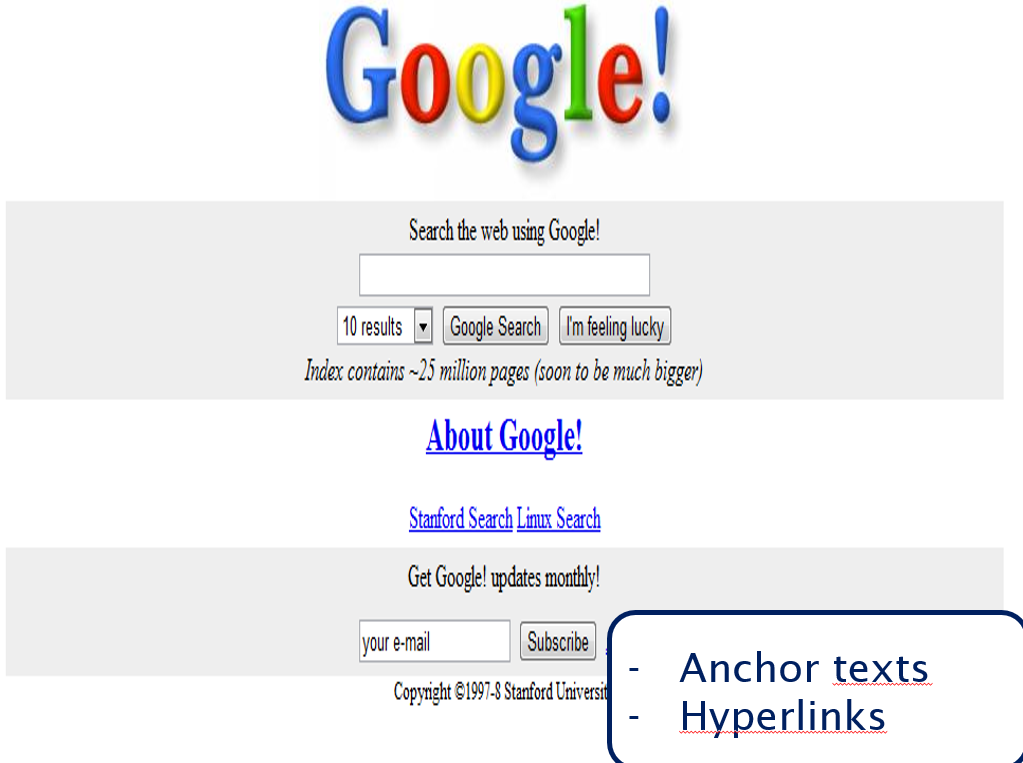
\includegraphics[width=0.65\linewidth]{images/googlehomepage.png}
    \caption{Google home page}
    \label{fig:googlehomepage}
\end{figure}
From a technical point of view there were two new things:
\begin{itemize}
    \item \textbf{Anchor text} (blue text that characterize an hyperlink); this is so important because if I look at the anchor text I can create an idea of the page where I land, so it helps me to understand what is the content of the page if I click on it; at the beginning it was so good, but unluckily the Web is not a good world (we will see later why, but remember Google bombing);
    \item \textbf{Hyperlinks} (links between pages); they allowed to create graphs where you could look at the edges between each page;
\end{itemize}
Then there was a \textbf{third generation} around 2005 and there were more sources like news, images, maps and Wikipedia. So people weren't looking only for pages but other things too, that's why pages weren't enough. This generation is known as \textbf{"multi-source"}.\newline
After few years there were only four search engines:
\begin{itemize}
    \item Google
    \item Bing
    \item Ask
    \item Yahoo!
\end{itemize}

In 2009 Ask disappeared in the sense that nowadays it exists and it works, but it can't be considered a world wide search engine due to his low percentage usage. After few years Yahoo! disappeared too in the sense that the backbone is not longer from them, but they take the results from Bing.\newline
The two biggest search engines are Google and Bing, there are even Yandex (Russian search engine) and Baidu (Chinese search engine). Their problem is that they are largely used in their countries, but around the world the usage percentage is very low.\newline
Around 2012 there was the \textbf{fourth generation} which is the current generation and it is related to different concept. Google introduced the \textbf{knowledge frame} which is a frame you find some knowledge.\newline
For example if you're looking for Galileo you will have the same page as in the past, but on the right you have a new frame that shows you some information related to your query like images, few lines of information like date of birth, written books and other stuff like that. It can be seen in the following image (Figure \ref{fig:galileo}).
\begin{figure}
    \centering
    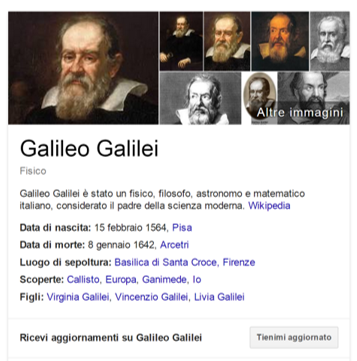
\includegraphics[width=0.55\linewidth]{images/knowledgeFrame.png}
    \caption{Knowledge frame}
    \label{fig:galileo}
\end{figure}
From this feature, people discovered that Google was using something new: \textbf{Knowledge Graph}. There are edges that encode relations between the nodes. The nodes can be people, cities, concepts, events. 
In our days this graph is huge there are billions of nodes, trillion of edges and thousands of relations between nodes.\newline
Graph algorithms are becoming crucial, they are so helpful.\newline
An example of Knowledge Graph is Wikipedia that it's a small Knowledge Graph (but not too small! In English is 6-7 million of pages). 
What is the feature of this Knowledge Graph? Every node (textual content) is a page and each node points to other nodes (anchor texts). Be careful that each anchor text is not the title of the node, for example a node can be "Diego Armando Maradona", but in other pages we can have anchor texts like "El Pibe De Oro" or "Maradona".
In the Knowledge Graph each page can be called \textbf{entity} too.
This concept is so important because suppose that we have:
\begin{quote}

\centering \textit{"Leonardo is the scientist that has painted Mona Lisa"}
\end{quote}
If our Knowledge Graph is enough developed we will have two entities (pages) that are "Leonardo da Vinci" and "Mona Lisa - painting".
This is important because all the nodes are in a graph so we can "expand" the graph and for example we will have that "Leonardo da Vinci" is linked with "Italy" or "Cartography" or "Science" that are nodes too.
The construction of Knowledge Graph depends on what is the context, for example there are some companies that are working on how to build a Knowledge Graph that it is "vertical" in the sense that it is specialized on a specific topic like Biology or Technology or Sport. On the other hand there are companies like Google that try to build Knowledge Graph for everything.
A problem to solve is that for example for "Leonardo", our system should be able to understand if "Leonardo" stands for "Da Vinci" or "Di Caprio" (if it exists).
This problem is called \textbf{polysemy} it happens when the same word has different meaning in two sentences that are similar. Look at the example below.
\begin{quote}
    \centering \textit{The paparazzi photographed the star}
\end{quote}
\begin{quote}
    \centering \textit{The astronomer photographed the star}
\end{quote}
If the algorithm that we build is "smart" it should be able to understand how much is important "paparazzi" or "astronomer" because then the meaning of "star" changes totally.
Another key point is \textbf{synonimy} and this happens when we use different words for the same concept. Look at the example below.
\begin{quote}
    \centering \textit{He is using Microsoft's browser}
\end{quote}
\begin{quote}
    \centering \textit{She plays with Internet Explorer}
\end{quote}
To solve this problem is to plug into the machine knowledge that these two different words must be mapped on the same page/node.\newline
Let's make a short resume about the evolution of Search Engines:
\begin{itemize}
    \item \textbf{Zero generation} (1991): it was the prehistory of search engines; just some metadata added by users; an example can be Wnaderer;
    \item \textbf{First generation} (1995-1997):  it used only on-pages (without anchor text); an example can be AltaVista or Excite or Lycos;
    \item \textbf{Second generation} (1998): it started to use off-page (anchor text); an example can be Google;
    \item \textbf{Third generation} known as "the need behind the query": it was focused on "user needs" rather than on query (if a page is a lot of clicked I have to take it into account) and it started to integrate multiple data-source; an example can be Google, Yahoo!, MSN or Ask; 
    \item \textbf{Fourth generation} known as "Information Supply" (current): it is used this description because it often happens that people write just one term in the query that's why you can't understand the user needs and for this reason you show to the user different "categories" like news, images and so on; otherwise if you have the profile of the user you can use his information to be more precise;
\end{itemize}
\subsection{What is the Paradigm Shift?}
To understand better how nowadays Search Engines work we have to talk about a \textbf{Paradigm Shift} that it is something more complicated that involves Computer Science because the search engines are part of this world.
Now we have <<devices 2.0>> that have their ID, Communication capacity, computing and storage and currently interaction ability and they work with Search Engines.
There are devices that "sensing" taking data from the world and then there are algorithm that "actuating" actions in the real world (IoT stuff).
Just to have an idea top level cars like Tesla have an interface that can access to Internet and navigate the Internet, this changed the interaction with search engine. For example now we have a voice interaction like Siri or Google Now. These tools changed the Web Engine because in the past when we people typed queries they were so lazy, they typed just 2-3 words for a query; now that there is a voice interaction people talk a lot and the queries are long (classic interaction of humans).
The "loop" changed because in the past the humans were obviously in the loop, but now the humans don't have to be inside the loop like IoT where devices answer to other devices.
If there is an interaction between two devices instead of human-device there are some things that change. For example we are able to look few results like 7-10 pages instead a device is able to look at thousands of pages.\newline
\subsection{Three types of data}
There are three main types of data:
\begin{itemize}
    \item \textbf{Opportunistic}: it is used this term because people are using something like credit card or telephone calls, but the result is that there are companies that take this data and use them in an opportunistic way for other stuff like finding friends in order to promote some advertisement;
    \item \textbf{Purposely sensed}: it is the typical pollution, temperature, movement; they are typical data used for something really specific;
    \item \textbf{User generated}: you ask people to contribute; this is typical social networks where you post photos or tweet;
\end{itemize}
Notice that the same data can be used for different purposes for example if there are some sensors that count each car that cross the street can be used either as purposely sensed either in an opportunistic way.\newline
Notice that search engines are not only things like Google, but even TomTom is a search engine where your query is a specific city or address (\textbf{searching routes}).
Even TripAdvisor is a search engine and you are not only searching by text, but even by distance so you have to take into account geography (\textbf{searching over Geo + labels}).\newline
Linkedin too is an information retrieval tool (\textbf{searching over labeled graphs}) where people are nodes and edges are connections between people.\newline
\newline
\section{Basics of Information Retrieval}
Now we start from a techincal point of view.
\subsection{Definition of Information Retrieval}
What is the definition of Information Retrieval? \textbf{Information Retrieval} (IR) is \textbf{finding material} (usually documents) of unstructured nature (usually text) that satisfies an \textbf{information need} from within \textbf{large collections} (usually stored on computers).
\subsection{Structured data vs. Unstructured data}
Usually we don't speak of Databases because they are table and they refer to \textbf{structured data} and the query is exact specified without ambiguity. In search engine we don't have this kind of query and the results aren't something really specific, but they are something that remind to your query (all the expressions that aren't well defined from a mathematical point of view).\newline
In our case we have \textbf{semi-structured data} like XML or JSON, we look the data as trees. To be honest almost no data is "unstructured" for example a slide has different zones like \textit{Title} or \textit{Bullets} and you can use operators like "contains".
Of course there are some issues like: "how do your process operator "about"?" or "how do you rank results?".\newline
At the end we have \textbf{unstructured data} that typically refers to free text and allows keyword queries including operators and there are some concept more sophisticated like "find all the web pages dealing with drug abuse".
\subsection{Boolean queries}
In search engine we have also \textbf{Boolean queries} because we have also the connector in the query. For example if I am looking for "Paolo Ferragina" implicitly I'm looking for "Paolo" AND "Ferragina", but the AND it's not an \textbf{Hard-AND}, it is a \textbf{Soft-AND}.\newline
If I search something on Google using two words that are too specific then Google "remove" one of them to relax the constraints.\newline
This search system is still used by Email, library catalog or Mac OS X Spotlight.\newline
Now let's go more in details why didn't the creator of Google used known structures like databases? To understand this let's look at an example.
Suppose that we want to build a search engine for Shakespeare poems, in the column we put the poems of Shakespeare (suppose that they are six) and on the rows we put the words that appear in each poem.\newline
Let's look at the following image (Figure \ref{fig:booleanmodel}).
\begin{figure}
    \centering
    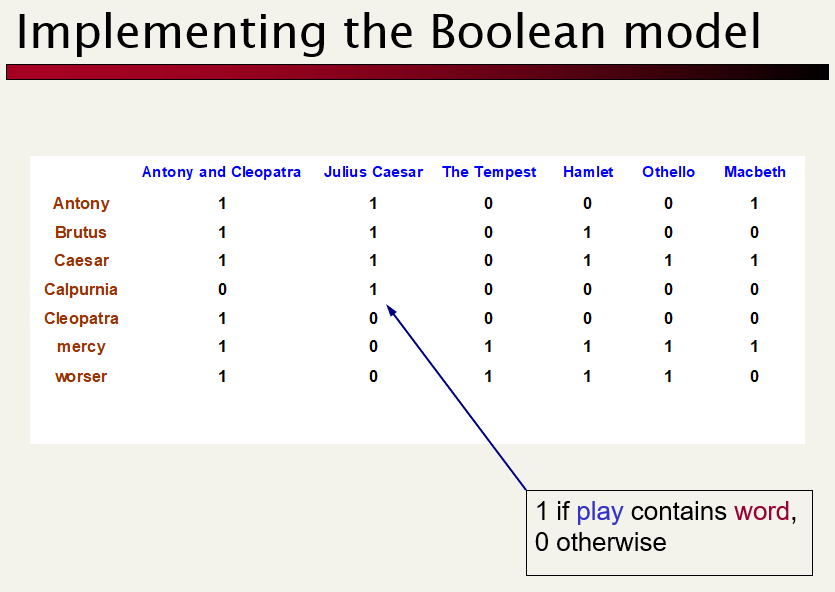
\includegraphics[width=0.8\linewidth]{images/boolean model.png}
    \caption{Implementing the Boolean model}
    \label{fig:booleanmodel}
\end{figure}
Now assume that the query is "Anthony AND Brutus", I have to find all the documents that contain Anthony and Brutus taking the two rows and doing a logical AND between them and if I get 1 I take the corresponding column otherwise I discard it.\newline
The problem of this approach is that there is a space problem because there are a lot of redundant zeros, this means that the matrix will be significant sparse. 
For example if I look at English Wikipedia there are over than 1 millions of pages (columns) and over 1 million of words (rows). If I create a matrix this matrix will be a matrix of size 1 million x 1 million and most of the cells will be sparse.\newline
Something different must be done: the data structure \textbf{inverted index} or \textbf{posting list}. For each term t (they are called \textbf{tokens}, sequence of character and numbers), we must store a list of all documents that contain t. We identify each document by a docID, a document serial number, like in the following image (Figure \ref{fig:inverted}). 
\begin{figure}
    \centering
    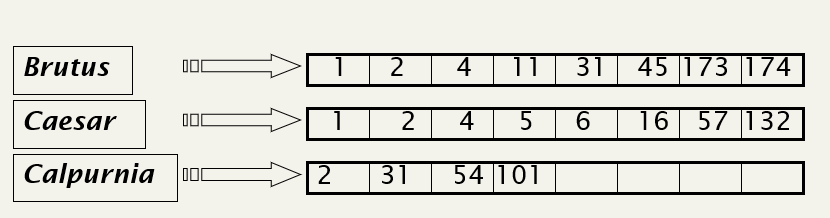
\includegraphics[width=0.75\linewidth]{images/invertedindex.png}
    \caption{Inverted index.}
    \label{fig:inverted}
\end{figure}
What happens if I want to insert a new docID? I just need to assign to it a docID then I need to scan it and looking the words, for each of them I go into the dictionary and if the term is new I add it to the dictionary otherwise I access to the list and put the docID (at the end obviously). Remember that the inverted index is ordered.
How do we solve an AND query? And why do I need to keep the lists sorted? If the lists are not sorted and I want to make an AND query between two lists, I need to start from the first one and for each element inside the first list I need to check ALL the elements of the second list. What is the complexity? If n and m are the lengths of the lists, I need to do n*m comparisons.\newline
If we sort the list it is easy and faster than the first solution. The algorithm works similar to merge in the Merge Sort algorithm. They start from the beginning and if they are equal I found a solution otherwise I let to advance the smallest one to the next position. I do this until I reach the end. In this case the number of comparison is equals to n+m. Obviously here it's better we do (n+m) comparisons instead of (n*m).
You can see the pseudo code in the following figure (Figure \ref{fig:pseudocode1}).
\begin{figure}
    \centering
    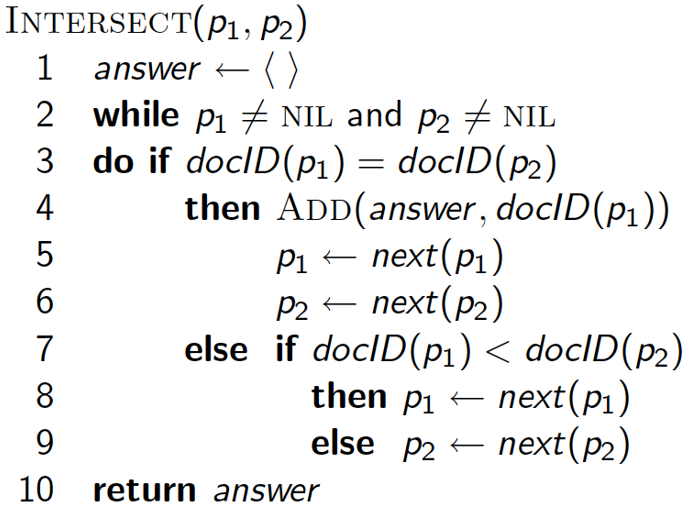
\includegraphics[width=0.75\linewidth]{images/intersectpseudo.png}
    \caption{Pseudo code}
    \label{fig:pseudocode1}
\end{figure}
At the end we can highlight two advantages of the sorting:
\begin{itemize}
    \item \textbf{Speed}: query requires just a scan;
    \item \textbf{Space}: store smaller integers thanks to the gap coding; Compressed they occupy 1-3 \% of original text;
\end{itemize}
What happens if the user specify more than two terms, but for example n tokens? What is the best order for query optimization? First of all for each of the n terms, get its postings lists, then AND them together. How do we choose the order? It is better to choose the shortest two, make the AND between them and so on.
For example look at the following image (Figure \ref{fig:optimization}), it is better to make the AND between Calpurnia and Brutus and the result with Caesar because they are the shortest two so it will happen that they can share at most two items (Calpurnia has length two and Brutus has length seven). Doing this I can optimize my space because the result will be shorter.
\begin{figure}
    \centering
    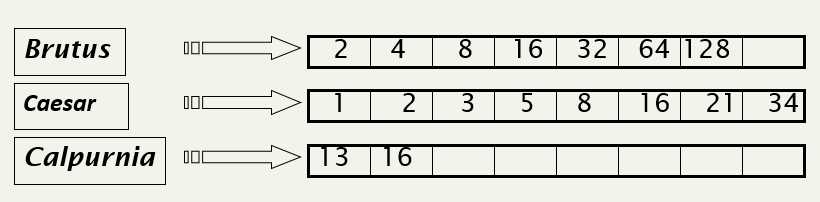
\includegraphics[width=0.75\linewidth]{images/optimization.png}
    \caption{How to process a query with n tokens?}
    \label{fig:optimization}
\end{figure}
We should highlight that the algorithm depends on the lists because the algorithm that we have seen in the figure \ref{fig:pseudocode1} it is not the best one in this case where we have a very long list and a very short list. It would be much better to do a binary search for each item of Calpurnia since it has a very short length. Otherwise I can process at the same time n lists, I just apply the algorithm that we have seen \ref{fig:pseudocode1}, but with n index. So we have seen different solutions with different performance (three possible solutions + the one with min heap where we store the min value with the index position).
\subsection{Optimizing queries}
Another question that we can make to ourselves is: Can we improve the scanning-based intersection? We have the skips and the recursive merge.\newline
The first idea that we can apply is the \textbf{skip pointers}. For every list we keep some extra information (we occupy more space). We divide the list into logical blocks, they don't exist they are just in our mind, each head of each block has a skip pointer to the head of the next block. There is an example in the following image (Figure \ref{fig:skip}).
\begin{figure}
    \centering
    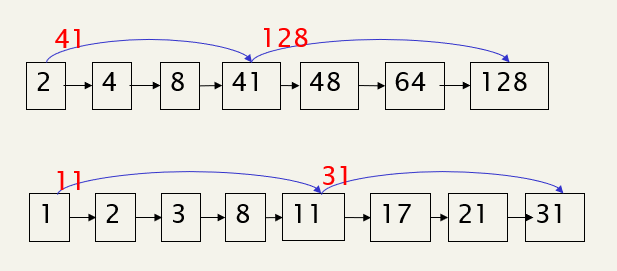
\includegraphics{images/skip.png}
    \caption{Skip pointers}
    \label{fig:skip}
\end{figure}
With a long block size I store less skip pointers and I save more space, instead with more skip pointers I save less space and obviously in the first case I have less probability to jump during scanning-based intersection, but if I do it I jump a lot of items. Otherwise in the second case I have more probability to jump, but I will jump fewer items. Usually the size of the block is chosen as if the size of the list is \textit{l} then the size of the block should be \textit{sqrt(l)}. If we know the distribution of the lists, that it's called \textbf{distribution aware}, we can change the size of the block list and the size has not to be the same for all the blocks it can change.\newline
Another way to optimize the query instead of skip pointers is the \textbf{recursive merge} without using pointers, but using pivots. It's called recursive merge for historical reasons, but the operation that it does is the intersection.\newline
Suppose that we have two lists and one of them is very short while the other one is longer. First of all we pick the median element (the one in the middle) from the shortest list and then we do binary search in the longer list. In the longer list can happen two things:
\begin{itemize}
    \item There is a match doing binary search;
    \item There isn't a match doing binary search;
\end{itemize}
In both the cases the binary search will return me a position, even if there isn't a match. Now I have that the two lists have been "splitted" in two parts and I can apply the same reason as before but for example if I am searching for the left element of the shortest list when I will do the binary search in the longer list I will do binary search with ranges [first position, position that returned me the iteration of before] because I am sure that after that position all the numbers are larger than my median element of the previous iteration.
In the following images it has been shown an example (Figure \ref{fig:recursivemerge}).
\begin{figure}
    \centering
    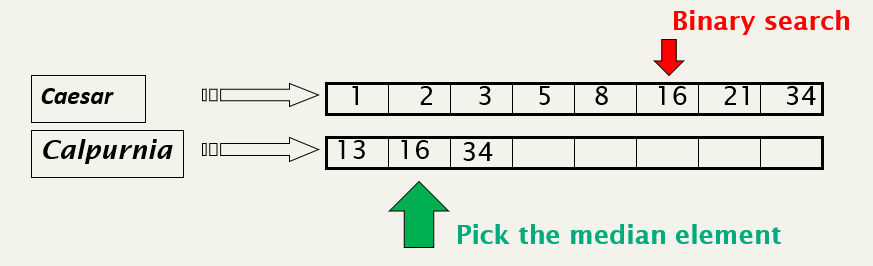
\includegraphics[width=0.75\linewidth]{images/recursivemerge.png}
    \caption{Recursive Merge}
    \label{fig:recursivemerge}
\end{figure}
This algorithm is very smart and if the median goes outside the last position of the longer list all the right part of the shortest list is removed. For example if 16 is greater than 34 then we can discard all the right part of the shortest list.\newline
What are the performance of this algorithm? If median is always out we have \textit{O(log m * log n)}. Every search takes \textit{log n} time, but I do this \textit{log m} times. We have to say that in practice this doesn't occur that's why we can't do an exact estimation of this algorithm easily.\newline
The worst case is that the median is always in the middle and the recursive relation is: \textit{T(n,m)=O(log n) + 2 T(n/2, m/2)}. This algorithm from a theoretical point of view is very elegant, but in practice is not used because it is based on recursion and it's very heavy for the machines to do that; in practice they use skip pointers.
\subsection{Queries with NOT or OR}
Until this moment we have only considered boolean queries with AND, but what happens if I want to computer NOT or OR? \newline
What is the result doing \textit{Brutus AND NOT Caesar}? When the two indexes are different then they are considered as a result otherwise if for example the min of the list 1 is equals to the min of the list 2 then I must not consider that docID.\newline
What is the result doing \textit{Brutus OR NOT Caesar}? In the case we have only OR we pick the docID in every case either if they are equal either if they are different. In this case we don't have only OR, but we have even NOT and here the situation is different. We should first of all consider \textit{NOT Caesar} that it is an huge list it will be very very long. This is not a nice query because we are "merging" a normal list ("Brutus") with an huge list that it is "NOT Caesar".\newline
Be careful that the NOT it is bad only with OR, but with AND it's not so bad.
\subsection{Different types of queries}
There are other types of queries in IR like:
\begin{itemize}
    \item \textbf{Phrasal queries} are queries like "Stanford University" (the quotes are included in the query); I expect to find out all the documents such that contain these two words one after the other one so I have to change my postings list because the structure that we have seen before doesn't work in this case;
    \item \textbf{Proximity queries} are queries like "Find Gates NEAR Microsoft"; I expect to find out all the documents such that contain "Gates" and "Microsoft" near possibly in a certain window of a certain size, for example windows\_size=3;
    \item \textbf{Zones/Fields queries} are queries like "Find documents with (author=Ullman) AND (text contains automata)"; 
    \item \textbf{Similarities queries} are queries like "Maradona", but I expect to find also "el pibe de oro"; these are queries where I check similarities among different tokens; in this case you need Knowledge Graph to make similarity checks;
\end{itemize}
To solve \textbf{Zone/Fields queries} we need first of all to define what is a zone. A zone is a region of the document that can contain an arbitrary amount of text (title, abstract, references). To do this we can build inverted indexes on fields AND zones to allow querying.\newline
There are two approaches:
\begin{enumerate}
    \item Build a posting list for each zone so I encode zones in dictionary; This one is the most used and it's very efficient;
    \item Build the posting list in a different way; the elements of the list are composed by the docID and the position where it occurs; in this case all the algorithms that we have seen don't work anymore because for example compression doesn't work anymore;
\end{enumerate}
In the following figure it has been shown an example (Figure \ref{fig:zonequeries}).
\begin{figure}
    \centering
    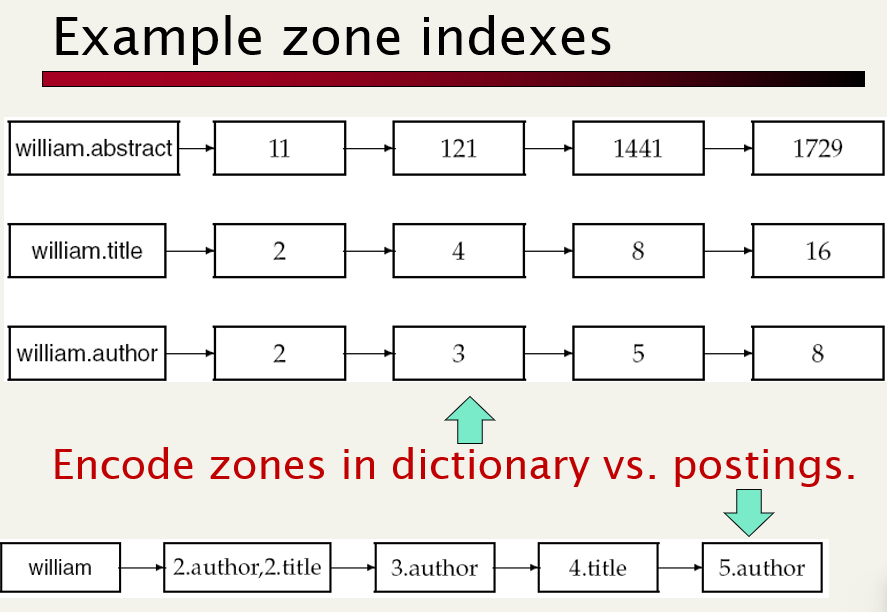
\includegraphics[width=0.75\linewidth]{images/zonequeries.png}
    \caption{Encode zones in dictionary vs. Postings}
    \label{fig:zonequeries}
\end{figure}
We are always talking on how to make queries and so on, but it's missing an entire world that it's the ranking search results. Boolean queries give inclusion or exclusion of documents, but often results are too many and we need to rank results. To rank results we can use: classification, clustering, summarization, text mining and etc.\newline
A lot of AI and Machine Learning on several kinds of features extracted from pages content and the Web for results selection and ranking.
\chapter{Structure of Search Engine}
In the following figure (Figure \ref{fig:searchengine}) it has been shown the structure of the Search Engine and all the main topics of this course.
\begin{figure}
    \centering
    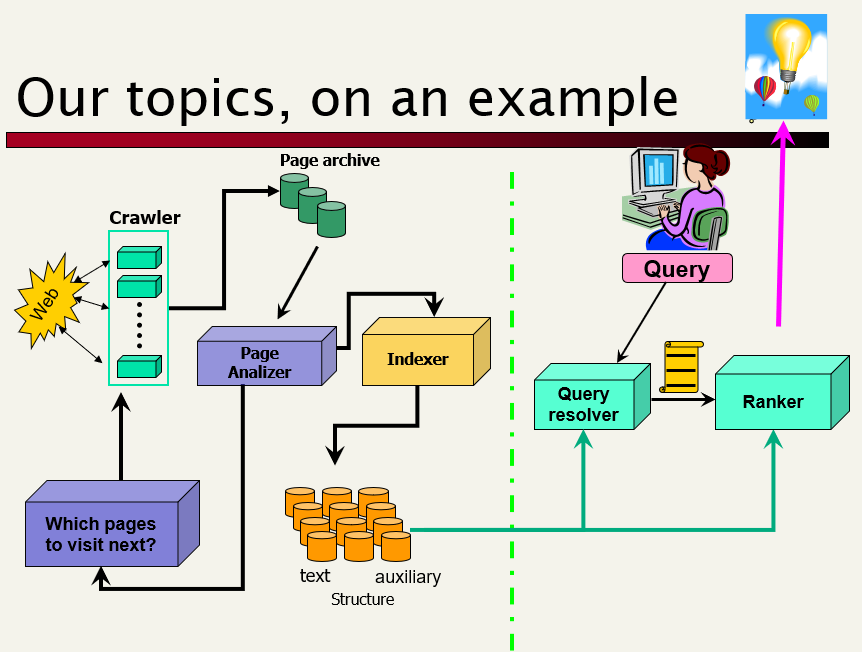
\includegraphics[width=0.85\linewidth]{images/search.png}
    \caption{Structure of Search Engine}
    \label{fig:searchengine}
\end{figure}
From the image we can see the \textbf{crawlers} that go around the Web and pick the documents. These documents are stored in a \textbf{Page Archive} and then they are analyzed because we have to build the dictionary. After that I have \textbf{parsed} the documents I have to \textbf{index} them (I have to build the inverted index that allows me to search faster). All these information are stored in an \textbf{archive} (WE ARE NOT TALKING ABOUT DATABASES). These things described are the "back-end" of the Search Engines that work 24 hours per day.\newline
On the other hand we have the "front-end" which is the part that you know. Whenever you issue a query the system gets your query and try to solve it and it solves the query accessing the index that the search engine has built. After this you have your documents and you sort them by relevance. At the end for example you show the first ten documents.\newline
In the next figure it has been shown many techniques that we will use to understand each element that we have just shown (Figure \ref{fig:functionssearch}).
\begin{figure}
    \centering
    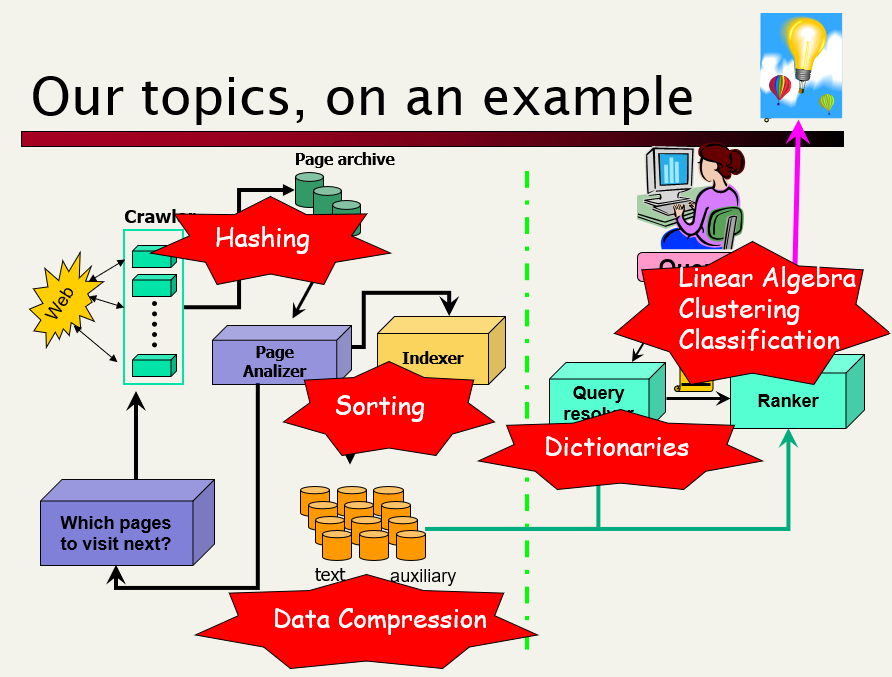
\includegraphics[width=0.75\linewidth]{images/functionsearchengine.png}
    \caption{Structure of Search Engine with functions}
    \label{fig:functionssearch}
\end{figure}
Let's give some facts in general. Let's describe the concept of "BigTable" it was very popular in 2006, but it was much older. In 2006 Google just shared it to the world and it's known as NoSQL Database that it's not a database. It's an huge table that you index by strings. You have strings on rows and columns. It's assumed to be an infinite table where you can do as operations put and get. The power of BigTable is that it's scalable, fault tolerance, secure, transactional and distributed geographically. In the following image it has been shown how it is (Figure \ref{fig:bigtable}).
\begin{figure}
    \centering
    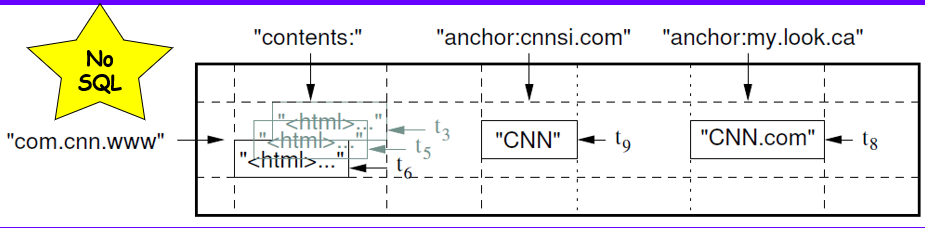
\includegraphics[width=0.75\linewidth]{images/nosql.png}
    \caption{BigTable}
    \label{fig:bigtable}
\end{figure}
Before that we go into the details we need to discuss about the Web in general. The Web has a very large size more than 1 trillion of pages, but nobody knows the real size that's why people talk about the size that it is indexed, but not the real size.\newline
The problem is that the Web is very dynamic because it changes always, it has been shown that only one third of the Web pages survive each year and only 20 \% of them are untouched, the others are always in changing. That's why extracting data from the Web is very difficult, then there are users and is difficult to match the "users needs" because 85 \% of the users look at only the first page of results that's why we must be very precise such that the first page of the results contains the right information.\newline
The Web is a graph whose size is 1 trillion of pages that each page has a size of 50-40k.
\section{Bow Tie Graph}
People think that the Web structure is \textbf{Bow Tie} and it is shown in the following figure (Figure \ref{fig:bowtie}).
\begin{figure}
    \centering
    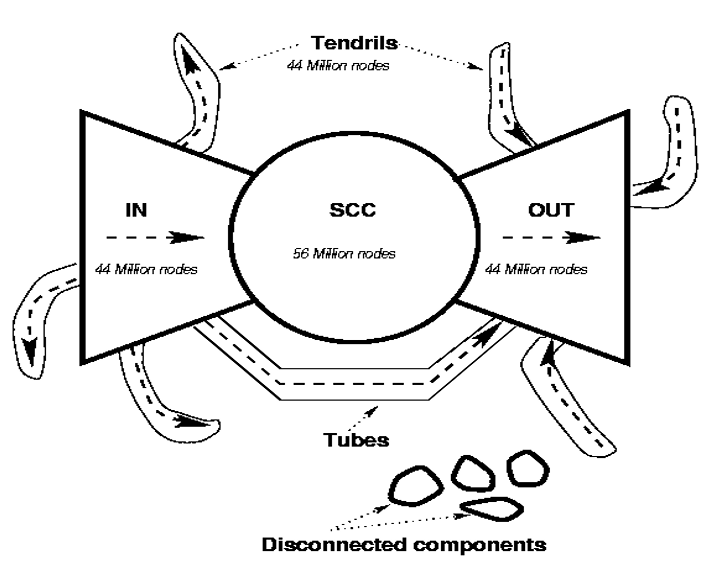
\includegraphics[width=0.75\linewidth]{images/bowtie.png}
    \caption{The Bow Tie - Structure of the Web}
    \label{fig:bowtie}
\end{figure}
The Bow Tie has different components:
\begin{enumerate}
    \item \textbf{Disconnected components}: they are part of the Web that are unreachable because they are not connected with other parts and typically they aren't interesting (if they are disconnected who cares about them);
    \item \textbf{SCC - Strongly Connected Component} (core): is a part of the directed graph, but this means that if you pick two nodes inside this component you can go from one node to the other and come back, so every pair of nodes is connected, "they are in a cycle"; this connected component is huge in the past was 56 million of nodes, now is much more bigger; one fourth of the Web is in this strongly connected component; there are other strongly connected components but they are smaller, this one is the bigger one;
    \item \textbf{IN - Connected Components}: is a part of the graph and if you pick a node inside this component you can go, through some paths, to other node always in IN or you can reach SCC; it had in the past around 44 million of nodes; remember that this has a lot of strongly connected components;
    \item \textbf{OUT - Connected Components}: is a part of the graph and if you pick a node inside this component it can be reached, through some paths, from other nodes always in OUT or nodes from SCC; it had in the past around 44 million of nodes; remember that this has a lot of strongly connected components;
    \item \textbf{Tubes}: they are sequences of pages or strongly connected components that allow you to move from IN to the OUT skipping the SCC; \textbf{remember that you can't have a path from OUT to the IN otherwise we would have an huge cycle and it would be SCC};
    \item \textbf{Tendrils}: they are sequences of pages that go from OUT or IN in some way, but they don't come back; for example it is a sequence of pages that go to my website and if in my website I don't have any hyperlink it will be stopped there;
\end{enumerate}
If I want to build a crawler it's clear that I have to start from a page that it's inside the IN component. In average these components (SCC, INN, OUT, Tubes + Tendrils) are each of them one fourth of the Web. Ideally I could take randomly four pages and one of them should stay in the IN component, but we can't do this because names aren't equally distributed. That's why people usually start from pages in the core and from them they try to reach pages from the other components.
\section{Crawling}
There are different synonyms of crawling, that's why we can hear even \textbf{spidering} or \textbf{bots} or \textit{downloader}. In few words they are programs/softwares/modules that go around in the Web and take pages (grab pages from the Web and bring them in Archive).\newline
To understand better how spidering works let's recall some notions like that the Web is a directed graph G=(N,E) where N are the nodes (pages), trillion of nodes, and E are the directed edges (hyperlinks between documents).\newline
There are some crawling issues:
\begin{itemize}
    \item \textbf{How to crawl?} we have to consider the \textit{quality} of pages, this means that we want to crawl first the "best" pages (best depends on the kind of search engine that we want to build, for example sports, news or general search engine); another key point to consider is \textit{efficiency} that's why we want to avoid duplication or near duplication in order to save space and time; we have to consider even the \textit{etiquette}, this means that the crawler has to satisfy some properties of the Web for example that he can't query many times the same server (it must not overload the server) or there are some directories that have not to be taken into account during the crawling. For this reason there is a specific file \textit{Robots.txt} that every crawler has to take into account when he acts; the last key point to consider is \textit{malicious pages} that can be divided in two different types: spam pages (offensive pages that the search engine doesn't want to crawl or not interesting pages) and spider traps (the crawler enter in these pages and start to waste time in useless pages)
    \item \textbf{How much to crawl?} we want a balance between new pages and pages that we have already seen, but we have to refresh them because these pages change like newspaper or social network; other two key points are the \textit{coverage} and \textit{relative coverage} because we know that the Web is huge and we can't cover all the pages and we can't spend time in refreshing pages that's why there is a trade-off between new pages vs. refresh pages;
    \item \textbf{How often to crawl?} the key points in this case are the \textit{freshness} and the \textit{frequency}; this issue decides how much frequent we have to come back to every page and it depends on the page because a newspaper need to be refreshed several times during the day while an university page doesn't need to be refreshed many times during the day;
\end{itemize}
In the following figure we describe what crawler does (Figure \ref{fig:crawlingexecution}).
\begin{figure}
    \centering
    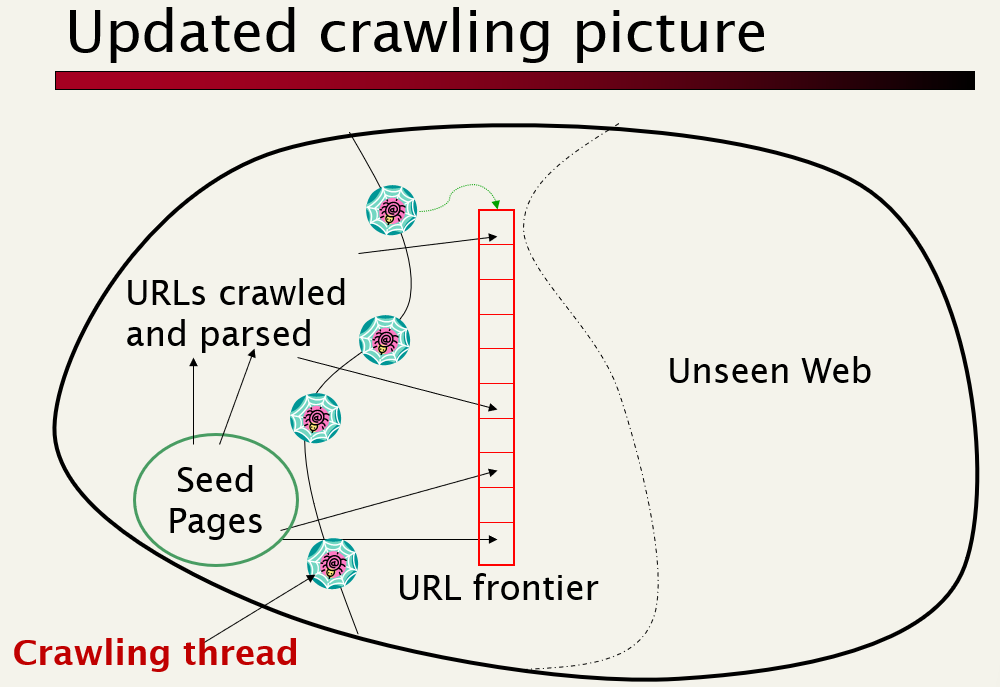
\includegraphics[width=0.75\linewidth]{images/crawlingpicture.png}
    \caption{Crawling execution}
    \label{fig:crawlingexecution}
\end{figure}
The crawler starts from a \textit{seed page} and his goal is to explore the Web graph. At a generic step we have some pages that are already crawled and are already been parsed and saved. At each step we have the \textit{URLs frontier} (it's a queue) that are URLs pointed from URLs already crawled and parsed, in other words are the set of pages that still have to be crawled. Be careful that not all the link of the URLs crawled and parsed go outside, but we can have links between pages already crawled and parsed. Remember that we don't have just one crawler otherwise we can't scale in order of the trillion of pages, but we have thousands of crawlers that work in parallel, they are independent and synchronized in the sense that they exchange information between them such that two or more different crawler don't crawl the same page if it's not needed.\newline
In the following image it has been shown a small example of a crawler with the flowchart of the algorithm (Figure \ref{fig:crawlingexample}).
\begin{figure}
    \centering
    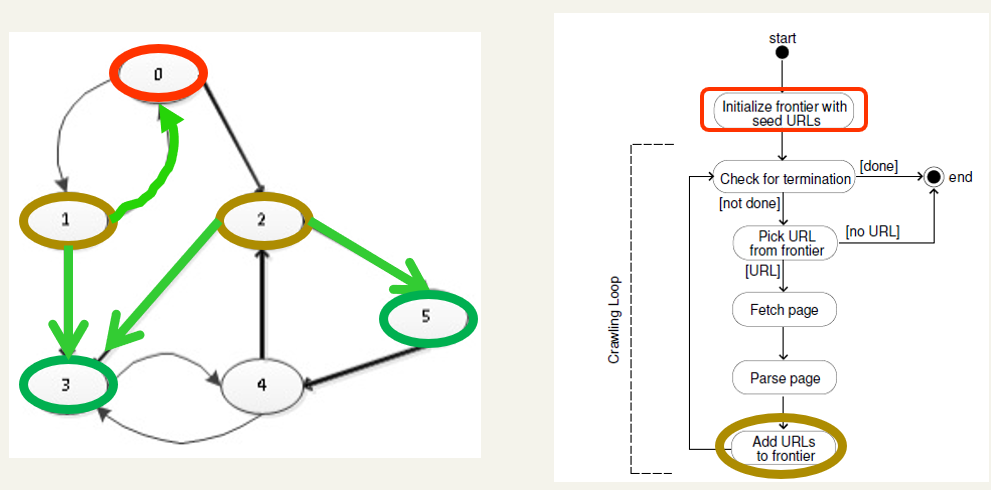
\includegraphics[width=0.75\linewidth]{images/crawlingexample.png}
    \caption{Example of crawling}
    \label{fig:crawlingexample}
\end{figure}
In this case I have just one crawler and the seed page is the node 0 and in the frontier we have "senape" nodes that are 1 and 2 from the frontier we pick the "best" node to be crawled according to the best policies that we choose. We can have many termination conditions (no other pages to crawl or time limit after that we start again from scratch). When we are in node 1 it can happen that we crawl again node 0 it depends on our design choice (freshness and frequency).\newline
Now let's look in more details the algorithm of the crawler (crawler "life cycle"). Assume for simplicity that we have just one \textbf{Crawler Manager} that it's a sort of dispatcher and extract URLs and for each of them it checks if the page has been not seen or the page has been seen, but it is an old version when one of these two cases is true it resolve the URL and assign the page to the \textbf{Assigned Repository}. Then we have one \textbf{Downloader} per page and the number of Downloader gives you the idea of parallelism that we can do. The Downloader \textbf{fetchs} the pages save them in a compressed form and assigns them to the Page Repository. At the end we have the \textbf{Link Extractor} or \textbf{Parser} (we have one of it per page) that takes pages from the Page Repository and extracts all the links in the page like href or links in javascript code and put them into the Priority Queue.\newline
In the following figure it has been shown the Crawler "life cycle" (Figure \ref{fig:lifecycle}).
\begin{figure}
    \centering
    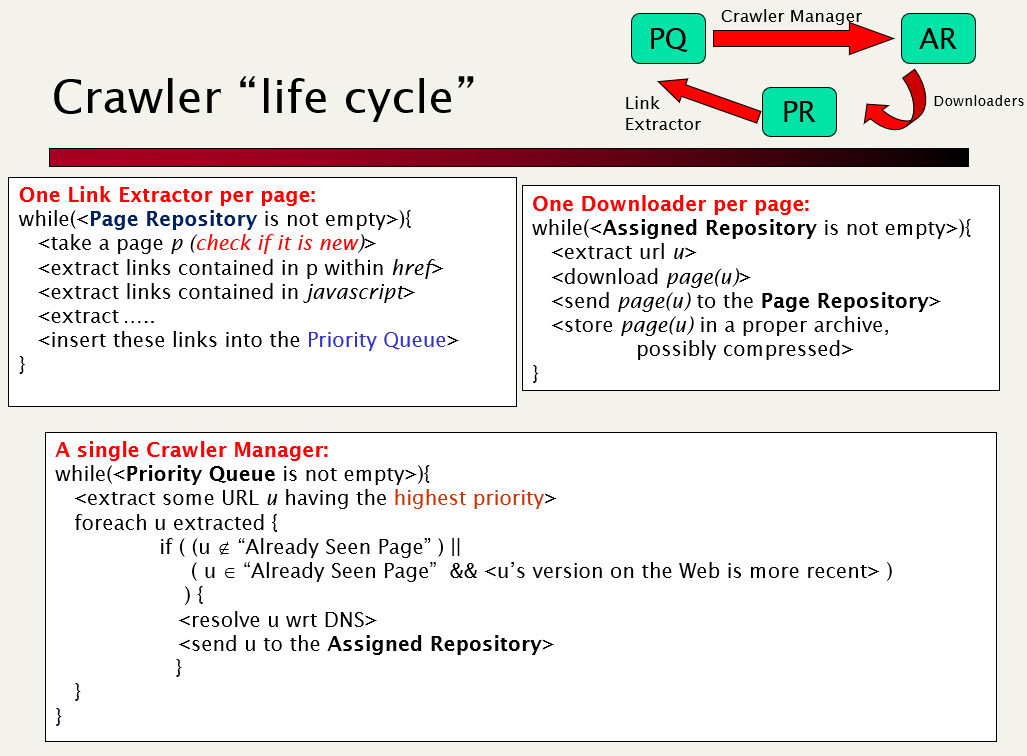
\includegraphics[width=0.75\linewidth]{images/lifecycle.png}
    \caption{Crawler "Life Cycle"}
    \label{fig:lifecycle}
\end{figure}
If we want there are a lot of open source crawlers on the web, but we need to specify just few parameters like seed pages, depth (how much deep I want to go when I enter in an host, this helps us to not enter into spider traps) and the domain of crawling. This is important to set because these crawlers are very fast and they can fill all your disk in small time.\newline
Now as we said we have the URLs frontier that has a set of pages, but given a page P, let's define how "good" P is. There are several metrics like:
\begin{itemize}
    \item BFS, DFS, Random;
    \item Popular driven where each page has a score like PageRank (obiously this is useful when you are re-crawling the Web and you already know the score of the pages otherwise if it's the first time you can't use this);
    \item Topic driven or focused crawling;
    \item Combined;
\end{itemize}
Another issue that we already talked about is: How to fast check whether the URL is new? To solve this problem we will use the Bloom Filter that it's a data sctructure that will help us with this issue.\newline
\section{The Mercator}
Now just for historical reasons we will discuss about a classic crawler that was one of the first crawlers (1999) that was used by AltaVista.\newline
In the following picture it has been shown the structure of Mercator (Figure \ref{fig:mercator}).
\begin{figure}
    \centering
    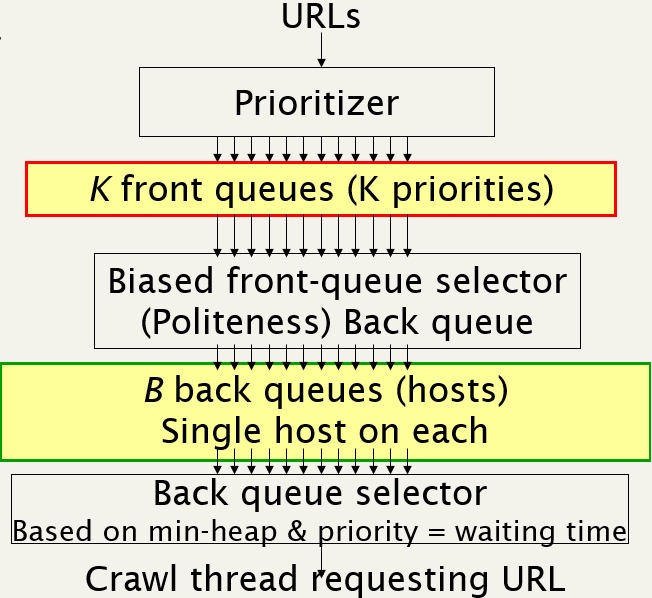
\includegraphics[width=0.75\linewidth]{images/mercator.png}
    \caption{Mercator structure}
    \label{fig:mercator}
\end{figure}
In yellow are indicated two data structures that are called queues: \textbf{K front queues} and \textbf{B back queues (hosts)} in particular they are priority queues with some features. The first one is called \textbf{Front queues} and as we already said it's a priority queue, we have K priority queues that it's a parameter that depends on the crawler. Each queue has a different priority that it's given from the \textbf{Prioritizer} and in a specific queue we can have more URLs with different domains. Then we have an algorithm that is a \textbf{selector} that picks randomly a queue from the Front queues depending on the priority (it's biased in the sense that it will pick more probably URLs from the queue K instead of the queue 1 because queue K means a larger priority than the queue 1). After this the selector put the URLs into the \textbf{Back queues} that are B, but the management of these queues is different because the distinction in the queues is done according to the host so in the same queue we will have all the URLs related to the same domain. Be careful that the crawler is able to manage only B domains. Now there is another \textbf{selector} that picks one URL from each priority queue (so we will have B URLs) and it will put them in a \textbf{min-heap} where the priority is the waiting time.\newline
Now let's go more in details with the two main parts.\newline
Starting from Front queues that manage prioritization, the prioritizer assigns to an URL an integer priority (based on refresh, quality, application specific) between 1 and K then it appends URL to corresponding queue, according to priority. In the following figure it has been shown a detailed image (Figure \ref{fig:frontqueues}).\newline
\begin{figure}
    \centering
    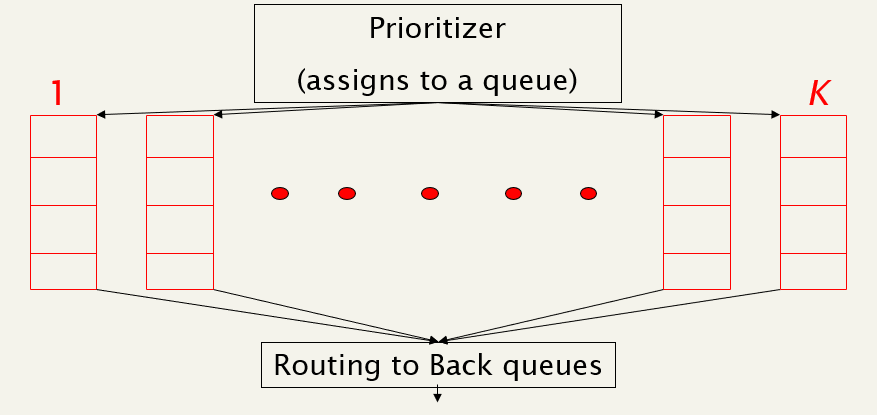
\includegraphics[width=0.75\linewidth]{images/frontqueue.png}
    \caption{Front Queues Details}
    \label{fig:frontqueues}
\end{figure}
A little bit more difficult are the Back Queues. As we said the Back Queues are B, the selector chooses a number randomly (it's biased) and goes to that queue and distributes the URLs among the B Back Queues, but there can be different problems like there is no space because either there isn't a queue with the domain of the picked URL or the queue is totally filled and I can't insert a new URL into the queue. For this reason the process of selecting URLs from the Front Queues is activated/triggered by the Back Queues when needed, we say that "Back queues enforce \textbf{politeness}" (only one connection per host is opened at time to not press to much the same host). Every queue is specialized to one single host, but host change during the running for example the i-th queue will refer to "di.unipi" then "corrieredellasera" and so on.\newline
Now what's missing is the last part, the URL selector picks from the B back queues the first item for each back queue (the queue is managed with a FIFO policy) and I insert them into the Min-Heap (with respect to some priority) that it's large B. Be careful that the priority in the Min-Heap is different from the priority that we had before because in this case it's a time interval that corresponds to the earliest time $t_e$ at which the host corresponding to the back queue can be hit again.\newline 
When we extract the min from the Min-Heap we are extracting the URL that has to be crawled first. It's advantageous to have a queue for each domain because let's suppose that we pick from the queue i-th the first item that has to be crawled at 4pm the "new" first item of that queue can't be crawled at 4pm too, but a bit later like 4.01pm.\newline
For this reason we check if the current time is larger than the time of the element in the Min-Heap we have to wait otherwise we can immediately crawl. The Heap must have always B items in particular one element for each queue.\newline
We have to discuss about a problem and is that if a back queue \textit{q} becomes empty and I ask to q a new element what happens? This means that no page from above arrived to that queue.\newline
The last part to talk about is about the crawl thread, first of all the crawl need an URL to crawl. It goes to the Min-Heap and it extracts the root of the heap (it's an URL at the head of some back queue q and then removes it). The crawlers waits the indicated time $t_{url}$. Then it parses URL and adds its out-links to the Front Queues.
Now can happen two cases when we extract an item from the back queue q:
\begin{enumerate}
    \item \textbf{The back queue q isn't empty} we pick the URL and add it to the min-heap with priority=waiting time $t_{url}$;
    \item \textbf{The back queue q gets empty} and the system doesn't have a new item to enter and it needs to fit the hole in the priority queue and for this reason it asks to the front queue to give him another URL (remember that the URL is chosen from the selector according to the priority); it can happen that the new URL is from a known host and we add it there (if the queue where we are adding it can be that the queue is full, but there is a "trick" between the size of B and K) otherwise if it's new we have a free queue that it's q and we assign the queue q to that host;
\end{enumerate}
Remember that Back Queues and Front Queues work in a \textbf{synchronized} way. A good heuristic to choose B is \textbf{B$=$(3 x threads)}.
\chapter{The Bloom Filter}
A problem that now we want to take into account is how do we fast check if a page is new or not. This problem looks trivial, but it's not because it requires time and space. We can't use an Hash Map where we put all the URLs because we crawl billion of URLs. To understand this better we can make an example let's suppose that we have 50 billion of pages (that's a small number against the real ones) and suppose that each page has 10 hyperlinks then this means that we have "seen" over 500 billion of pages. In average each URL occupies 1000 chars this means that we store 500.000 Tb (500 Pb) just to know which URLs we have already seen!\newline
At that time AltaVista used the disk access with caching, but nowadays a modern approach is the Bloom Filter that it's an archive. Supposing that we have 500 billion of URLs it occupies around 50 Tb that's very efficient.\newline
\section{Bloom Filter}
The Bloom Filter has been created in 1970 and it's a data structure that in the first times it didn't have any success, but when search engines came out it had a lot of success because was so helpful. This data structure has some good features and some bad features. First of all is good because it occupies very few space and this is important because we deal with a lot of items; on the other hand this data structure is not always "correct" that's why is called \textit{one-side error data structure} in the sense that the answer is Yes or No and if the answer is No we know for sure that it's correct, but if the answer is Yes it can be probably wrong the answer. Our goal is to estimate the probability of error (we will see that it's a low probability).\newline
Let's look at the structure of the Bloom Filter:
\begin{itemize}
    \item It's a binary array of length m, B[1,m];
    \item Consider a family of k hash functions that map a key (URL) to a position (integer) in B;
\end{itemize}
\textbf{How do we add URLs to Bloom Filter?} Whenever you have a key (URL) you compute k hash functions that will return you k positions (integer) each one of these position is set to 1 (if it's 0 we change it with 1 if it was already 1 we don't change it), this is just a binary array. In the following image it has been shown an example (Figure \ref{fig:bloomfilterexample}).


\begin{figure} [h!]
    \centering
    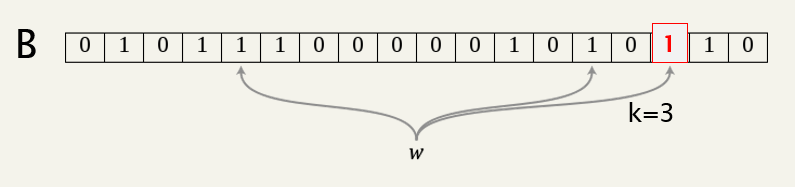
\includegraphics[width=0.75\linewidth]{images/bloomfilterexample.png}
    \caption{Bloom Filter example}
    \label{fig:bloomfilterexample}
\end{figure}
Remember that we can't delete (some positions becomes 0 where there are other URLs that go to that positions), we can just insert and get (that can be wrong for some reasons already introduced).\newline
\textbf{How do we check if an URL is already in the set?} Whenever you have a key (URL) you compute k hash functions that will return you k positions (integer) and if at least one of them is equal to 0 then I know for sure that the key wasn't in the set. Instead if when I compute the hash functions all the positions that I get are equal to 1 then the answer is \textit{maybe the URL was already in the dictionary} because these k positions could have been set to 1 by my URL or by other URLs.\newline
I don't know if the key (URL) was already in the dictionary because this data structure throws away the keys (URL) after that it insert them into the Bloom Filter. I don't store the keys because the keys are URLs and each URL requires too much space around 1000 chars one URL doing this I need to store only one array of size m. The space that I require is m bits because we have an array of size m and each cell of the array requires one bit (0 or 1). \newline
In the following image it has been shown an example of Bloom Filter in a Biology situation (Figure \ref{fig:biology}). Looking at the image the set S that shows the keys inside the Bloom Filter is thrown away that's why when I receive a new key I compute again the hash functions.
\begin{figure} 
    \centering
    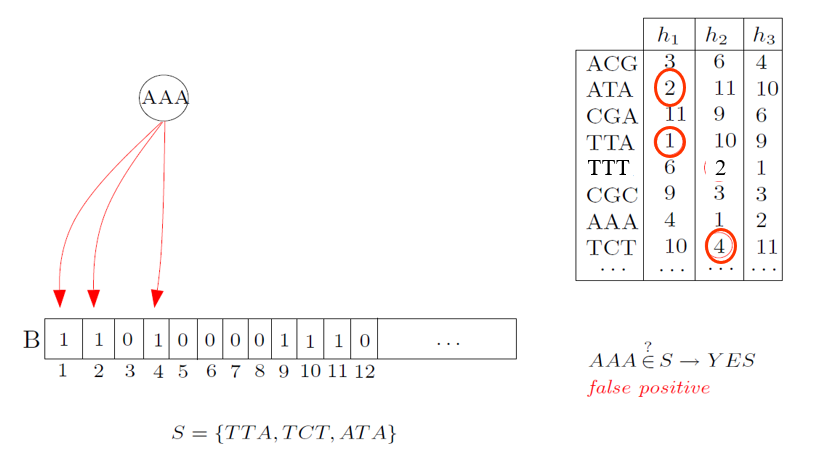
\includegraphics[width=0.75\linewidth]{images/bloomfilterbiologic.png}
    \caption{An example of Bloom Filter in Biology field.}
    \label{fig:biology}
\end{figure}\newline
\textbf{What is the probability of making an error?} The probability of making an error (\textit{false positive}) is equal to $(1-e^{-kn/m})^k$ where \textit{k} is the number of hash functions, \textit{n} is the number of the keys and \textit{m} is the size of the Bloom Filter. Furthermore it's possible to compute the minimum of this function whenever \textit{m} and \textit{n} are fixed. In fact when they are fixed we should choose $k=(m/n)ln2$ to compute the minimum we just do the derivative and set it to 0.\newline
If we put the value of k chosen following the previous rule into the formula that we have seen we obtain this:
\begin{equation}
    (1-e^{-kn/m})^k=0.62^{m/n}
\end{equation}
The size of m is larger than of n because if the array is too small I would have an array with all ones. Sometimes it's not worth to choose k like $k=(m/n)ln2$ because it can happen that $m/n$ is a large number so I would spend a lot of time checking the positions of the array (spend too time).\newline
From the previous formula we can see how if I increase the value of m then the probability of false positives goes down exponentially because m is at the exponent. Another way to understand how strong is this data structure is looking the formula from another point of view: suppose that we have $m/n=30$ I can write this as $m=30*n$ bits this means that if I use 30 bits for each key (because n is the number of keys) I can achieve a small error probability (obviously if we choose k in the best way as $k=(m/n)ln2$).\newline
If we want more into the details with the formula let's see what it happens when we choose in an appropriate way k, the \textit{general} formula becomes $(1/2)^{m*ln2/n}$ and $(0.62)^{m/n}$ comes from the fact that $(1/2)^{ln2}$ is equals to 0.62.\newline
Now let's have a fast look at the differences between the Bloom Filter and the classic Hash Table. With Bloom Filter we require a space of m bits to store n keys. Let's see what happen with the classic Hash Table, we will have a length called m' that it's proportional to n, the number of keys, $m'=\Theta(n)$ and the average list for a specific cell is $O(1)$ that it's efficient when we have to access to the list. The problem with this technique is that we must store the keys let's have a look at the space that we require. The classic Hash Table requires \textit{space of T + space of the lists}, let's go deeper with these two value. The space of T is equal to \textit{8 bytes * m'} and the space of the lists is equal to \textit{(L+8 bytes)*n} (8 bytes = space required by a pointer and L = space required by a key). Since we said that $m'=\Theta(n)$ so m' is proportional to n for simplicity assume that \textit{m'=n}. At the end we will get \textit{8n + (L+8)n} that it's equal to \textit{(L+16)n bytes}, let's transform bytes in bits to make a comparison with Bloom Filter (we must multiply by 8) \textit{(8L+128)n bits}.\newline
Let's compare the two techniques and consider the case where \textit{m < (8L+128)n}, before we said that \textit{m} should be considered bigger than \textit{n} and we can see it like \textit{n * c} (c = constant >= 1).\newline
From this we can infer that \textbf{Bloom Filter is more space efficient than HashTable iff} \textit{c < 8L+128}.\newline
At this point recall what is the error for the Bloom Filter $error=(0.62)^{m/n}$ hence $error=(0.62)^c$. \newline
The HashTable gives you always the right answer, but it occupies a lot of space instead Bloom Filter gives you an answer with a low error probability. This structure is used by some databases and virus detector.\newline
\section{Spectral Bloom Filter}
Now we are going to consider a new variation of Bloom Filter that it's able to consider counting and deletion operations that it's called Spectral Bloom Filter (SBF). The Spectral Bloom Filter is used by Search Engines because they keep into account \textit{query logs} because they want to remember the queries done by the users such that they can do statistics on queries. This variation is a dynamic data structure because it allows operations like deletion and counting.\newline
Let's show a definition of SBF \textit{M=<S, $f_x$>} is a multi-set were: S is a set and $f_x$ is a function returning the number of occurrences of x in M.\newline
There are some original features of this variation:
\begin{itemize}
    \item Space usage is slightly larger, but the performance are better;
    \item Insertions/Deletions are possible with some tricks;
    \item It manages streaming data (data that arrive after one the other and I want to manage them in the order as they arrived);
    \item It allows \textit{iceberg queries} (given x, check if $f_x > T$ dynamic threshold) and aggregate queries (SELECT count(a1) FROM R WHERE a1=v);
\end{itemize}
The B vector is replaced by a vector of counters $C_1$, $C_2$, ..., $C_m$ and $C_i$ is the sum of $f_x$ values for elements $x \in S$ mapping to i. This means that the approximations of $f_x$ are stored into $C_{h_1(x)}$, $C_{h_2(x)}$, ..., $C_{h_k(x)}$. Since we can have conflicts in the same cell the $C_i$ provides approximations.\newline
In the following figure it has been shown an example (Figure \ref{fig:minimumselection}).
\begin{figure}
    \centering
    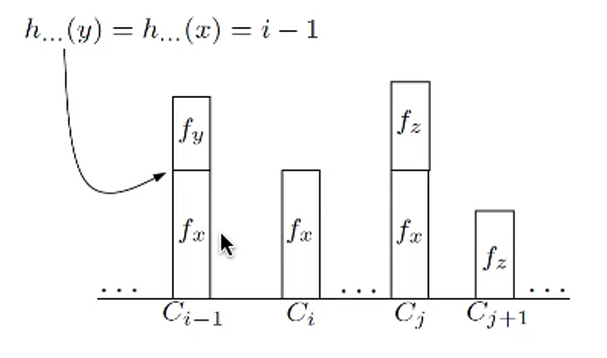
\includegraphics[width=0.75\linewidth]{images/minimumselection.png}
    \caption{Example of Spectral Bloom Filter}
    \label{fig:minimumselection}
\end{figure}
From the image we can see:
\begin{itemize}
    \item $C_{i-1}$ is not a good approximation of $f_x$ (neither of $f_y$) because I had a collision;
    \item $C_i$ is an exact approximation of $f_x$;
    \item $C_{j+1}$ is an exact approximation of $f_z$;
\end{itemize}
Obviously I would like to not have collision such that the cell dedicated to a specific item gives me the exact number of occurrences. Let's highlight that I can have only overestimation, I can't have underestimation because I just sum items. I hope that when the k hash functions give me k positions at least one of them is correct and that's why I always take the minimum (it's clear that it's not always correct).\newline
Let's see in more details the algorithms of \textit{insertion} \textit{deletion} and \textit{search}.
\begin{itemize}
    \item The insertion is simple because what we do is just for each hash function we compute the position and we increase by 1 that position;
    \item The deletion is simple too because it's like the insertion, but instead of summing we decrease each counter by 1; we assume that we do deletion only of things that we already have we can't delete things that we don't have;
    \item Searching for an element x needs to compute the positions for all the hash functions and then return the \textbf{Minimum Selection} (MS) value between all the values that I got;
\end{itemize}
Notice that in this case each cell has counter instead of just one bit so we should choose how many bits assign to them. For example if we choose 5 bits then it means that we can represent at most $2^5$ counters.\newline
\textbf{How can we prove that the Spectral Bloom Filter has the same error of Bloom Filter?} Let's reason on this, the probability of have an error is the probability that all the cells that I check have a collision, but this is exactly the error probability of the Bloom Filter (it fails when all the cells that I check are ones and the key is not in the set). The error is the same as for Bloom Filters.\newline
\textbf{Theorem:} For all \textit{x}, it is $f_x <= m_x$. Furthermore $f_x != m_x$ with probability $E_{SBF}= \varepsilon \approx (1-p)^k$. (Here the formula is the same as Bloom Filter, but the value \textit{m} is the number of cells and not the number of bits).\newline
\textbf{Proof:}
\begin{itemize}
    \item The case $m_x < f_x$ cannot happen;
    \item The event $m_x > f_x$ is "all counter $C_{h_i(x)}$ have a collision", that corresponds to a "false positive" event of classical BF;
\end{itemize} 
We have mainly two challenges to improve:
\begin{enumerate}
    \item allow insertion/deletion keeping low $E_{SBF}$;
    \item dynamic array of variable-length counters (suppose that I'm using a lot of bits for each cell and in one cell I have counter equals to 1, I'm wasting space), but we will not see how to manage this problem;
\end{enumerate}
To solve the first problem we introduce the idea of \textbf{Recurring Minimum} (RM). To better understand this concept let's have a look at this simple figure (Figure \ref{fig:recurringminima}).
\begin{figure}
    \centering
    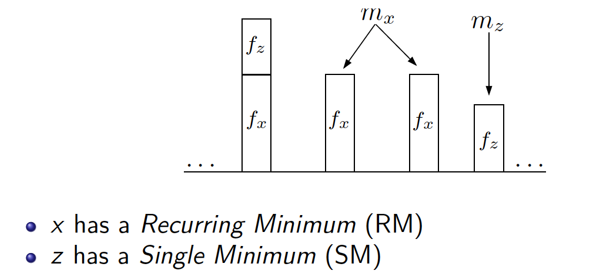
\includegraphics[width=0.75\linewidth]{images/recurringminima.png}
    \caption{Example of Recurring Minimum}
    \label{fig:recurringminima}
\end{figure}
Let's give a definition of Recurring Minimum (RM): an element has a RM iff more than one of its counters has value equal to the minimum. The idea is that if we have a RM it's very improbable that the value it's wrong because it means that there are other items that accessed to that positions and increased always the same positions.\newline
Instead if the minimum recurs just one time then it's called \textbf{Single Minimum} (SM). In general the algorithm says that if we have a RM we consider that value as our result, but if we have a SM we do other stuff because we aren't sure about that result.\newline
\textit{Basic idea:} We operate as in MS (Minimum selection), but over two SBF.
\begin{enumerate}
    \item For item x with RM we use $m_x$ as estimator which is highly probable to be correct: hence $E_{SBF_1} < \varepsilon$ (because the minimum occurs more times than one time);
    \item For item with a SM we use a secondary SBF which is $|SBF_2| \ll |SBF_1|$ and thus can guarantee $E_{SBF_2} \ll \varepsilon$;
\end{enumerate}
We use more space which could be used for enlarging the single BF, but it has been shown that improvements may be remarkable that's why we use this variation!\newline
Now let's analyze how we do operations with Recurring Minimum.\newline
\textbf{Insertion}: first of all we increase all the counters of x in $SBF_1$ then we check if x has a RM in $SBF_1$ we stop otherwise we go to $SBF_2$ and we look for x; now we can have two cases: the first one is that x is already in $SBF_2$ and we only need to increase by 1 all the counters otherwise we set x in $SBF_2$ as the minimum value of x in $SBF_1$ (we increase using the minimum so the cells equal to 0 become equal to the minimum and the cells different from 0 are increased using the minimum for example if we have 0 and 1 and the minimum is 3 then we get 3 and 4).\newline
\textbf{Deletion}: is the inverse of the insertion so first of all we decrease all the counters of the $SBF_1$ then we check if x has a SM in $SBF_1$ if this is true then we go to the $SBF_2$ and we decrease all the counters of x in $SBF_2$ (if any).\newline
\textbf{Lookup/Search}: first of all I check the value of x in $SBF_1$ and if I have a RM I can stop otherwise if I have a SM I go to the $SBF_2$ and I check if the value of x is greater than 0 I take it as a result otherwise I take as result the minimum of the $SBF_1$.\newline
In the following image it has been shown the pseudo-code of these three operations with SBF with RM (Figure \ref{fig:insdelloo}).\newline
\begin{figure}
    \centering
    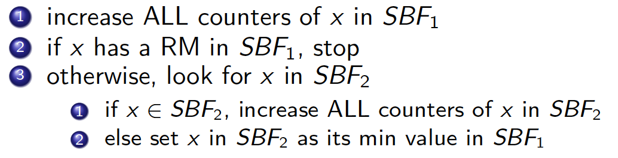
\includegraphics[width=0.75\linewidth]{images/insertion.png}
    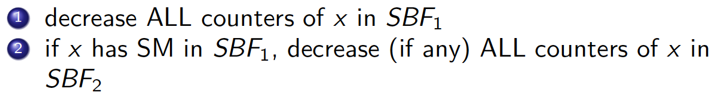
\includegraphics[width=0.75\linewidth]{images/deletion.png}
    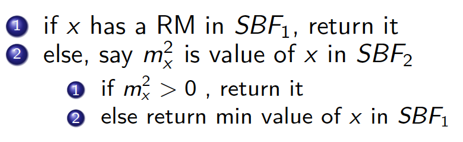
\includegraphics[width=0.75\linewidth]{images/lookup.png}
    \caption{Pseudo-code of insertion, deletion and lookup}
    \label{fig:insdelloo}
\end{figure}
\textbf{Notice} that if we know a prior all the dictionary of items we can avoid the problem, that a key from a RM become a SM inserting a new key, this never occurs. To avoid this we can initialize the structure inserting all the keys with value 1 only in the First SBF such that we surely have all the keys present and then we start counting. It never occurs that a new key arrives and destroys a RM that we had before. If this occurs the key was already present before so the clashing cell was already identified as a "colliding" cell. Obviously we can do this only when we already have all the dictionary.\newline
\chapter{Parallel Crawlers}
In this chapter we will discuss about a problem that it's how to distribute the work among different crawlers that work in parallel for example how we have to assign tasks to the downloaders that will download pages.\newline
In order to make this process efficient we have to avoid the duplication of work in the sense that whenever some pages have to be crawled they must be assigned only to one single bot/crawler/spider.\newline
There are two approaches to solve this problem:
\begin{itemize}
    \item \textbf{Static assignment:} this is the simplest assignment and suppose that for some reason we are able to partition the web and we assign each part of the web to a specific crawler; the goal is to have a balance partition s.t. each crawler has the same amount of work to do; obviously we can't assign to each crawler a specific domain because each domain has different size (".it" is smaller than ".com"); ideally this would be nice, but it's not affordable;
    \item \textbf{Dynamic assignment:} this is something where we have a coordinator that leads the crawler and it distributes URLs to the crawlers trying to keep balanced the work; in this case to guarantee that the work is balanced we can use an hash function \textit{h} that takes an URL and returns as output a number that it's in the range between [0, c-1] (this is simple to be build) where \textit{c} is the number of the crawlers/downloaders; that's it if the hash function is sufficient good taken a set of URLs it will distribute them in a balanced way the URLs between all the crawlers;
\end{itemize}
As we said we have these two approaches, but the best one that it's used is the dynamic assignment. Now let's have a look at what can happen.\newline
\textbf{How do we manage fault-tolerance} because if a crawler dies or a new crawler is added we need to recompute again an hash function and all the URLs have to be assigned again. To solve this problem there is a solution that it's called \textbf{Consistent Hashing}.
\section{Consistent Hashing}
This solution has been proposed by an MIT group, the same that created Akamai the largest content delivery network, but now let's look at the idea.\newline
Assume to consider a space like a ring with integer numbers from [0, $2^k-1$] (to implement this we can just use modulo and we get it). Now you can have one hash function or more hash functions. For simplicity we can consider just one hash function and the domain is $U$ (space of the objects that I want to distribute so they are servers/crawlers or items/URLs) and the co-domain is the ring so [0, $2^k-1$] so this means that the hash function is in modulo $2^k$.\newline
Assume that you have a set of servers $s_1$, $s_2$, ..., $s_n$ to map then we take the hash function and we apply it to all the server getting $h(s_1)$, $h(s_2)$, ..., $h(s_n)$. These values are integers in particular they are positions of the ring. This is the first distribution and it's totally random. Now we do the same thing with my items $u_1$, $u_2$, ..., $u_m$ and we will get as result $h(u_1)$, $h(u_2)$, ..., $h(u_m)$ that are always integers in particular they are positions of the ring.\newline
Notice that it can happen that the same position is assigned to a server and to an url.\newline
The question now is \textbf{how do we map URLs to servers?} we just need to take the ring and read it clock-wise or anti clock-wise and assume that we choose it clock-wise we will have that \textit{all the URLs that occur before the server $s_i$ will be assigned to it up to the first server that we meet}, in other words we can imagine the server as the head of this list.\newline
This is the idea, but the question is \textit{why is this advantageous?} Suppose that one machine is broken then we don't have to remap all the objects, like the previous solution, but we have to remap only the objects assigned to that machine and to do that we just add them to the \textit{tail} of the next server.\newline
On average if \textit{n} is the number of the URLs and \textit{s} is the number of the servers then $n/s$ will be the \textbf{average number of items assigned to one server}. So if one server is broken we have to remap only $n/s$ objects instead of n.\newline
\textbf{What happens if I add a new server?} It's exactly the same because I put the new server in the middle of a trail and I will "split up" the number of items assigned to the previous server. We can see insertion as a "split" and deletion as a "merge".\newline
There is a property that can be proved about \textit{sampling} if you want guarantee that $n/s$ is the right distribution of objects instead of sampling s objects you sample $s*log(s)$ and then among these $s*log(s)$ you pick just one over s; in other words you map the server on the ring and then the distance between two servers is log(s) thanks to this we are guaranteeing that the distribution is more concentrated over $n/s$ (each server gets replicated log s times).\newline
\section{Software Crawlers}
There are some open source software to crawl the web like Nutch from Apache Foundation or Scrapy that it's written in Python (from this it comes the suffix "py"). To use these software you just need to specify which are the seeds (starting page) and the bounds (the domain) and at the end you can specify the level, how deep you want to go. Usually it's recommended to keep the level <= 2 that allows you to crawl a lot of pages otherwise the disk can be filled in few time.
\chapter{Compressed storage of the Web Graph}
This new chapter it is still related to crawling in particular we will see what happens when I download the pages.\newline
The pages that I have in my archive will represent a graph and we will have an huge graph with billions of nodes and multi billions of edges so I want to represent it in a compressed form due to its dimensions.\newline
Nowadays this topic is even more important because there are Graph DB that are DBs where information is not stored in terms of tables, but in form of graphs and the queries that you will do are queries on graphs. Many DB for banks are better encoded with a graph structure instead of a table structure. The most common GraphDB are Neo4J and Arango DB.\newline
The concept that we will introduce is the \textbf{Web Graph Compressor} that was invented by some professors in Milan.\newline
The Web Graph Compressor has three key properties:
\begin{enumerate}
    \item \textbf{Skewed property:} the probability that a node has \textit{x} links is $1/x^\alpha$ where $\alpha \approx 2.1$, this kind of distribution where $\alpha$ is a constant is called \textbf{power-law}; remember that we should have a normalization constant such that the sum of all the value gives us 1;
    \item \textbf{Locality:} most hyperlinks from a page \textit{u} point to pages in the same host; 
    \item \textbf{Similarity:} given two pages \textit{u} and \textit{v} that are in the same host, they share many hyperlinks (or they point to same pages);
\end{enumerate}
To understand better the Skewed property we will make a plot to show that pages with one hyperlinks are a lot instead pages with a lot of hyperlinks are few, we have a long tail. It can be seen in the following picture (Figure \ref{fig:powerlaw}) and it's the typical structure of the \textit{power laws}.
\begin{figure}
    \centering
    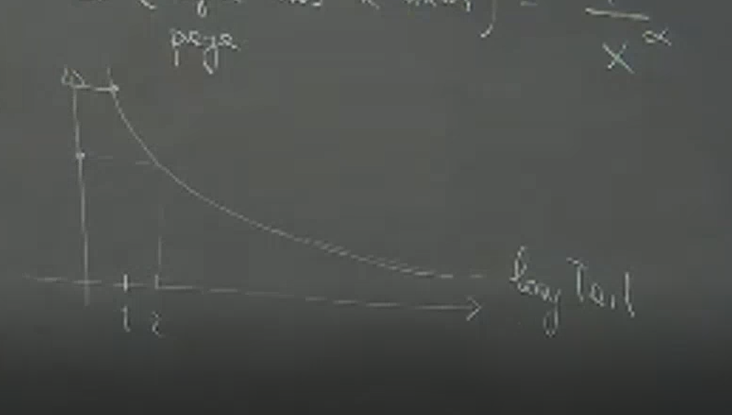
\includegraphics[width=0.75\linewidth]{images/powerlaw.png}
    \caption{Plot where the x is the number of hyperlinks and the y is the probability of having x hyperlinks/frequency of pages with x hyperlinks.}
    \label{fig:powerlaw}
\end{figure}
\section{Skewed Property}
Notice that the power law is based on \textit{probability} so in the plot you have as y the probability; in the real applications you don't know the probability, but you know the frequency of the pages with x hyperlinks.\newline
This property has been found for many crawlers in the Web that's why it's considered a rule in the Web. The power law is used a lot in Data Science, but it's very difficult to  see by eyes if it's a polynomial distribution or exponential (they have a similar structure) and for this reason researchers decided that given $y=x^{-\alpha}$ (the formula that we have already seen written in a different way) then they apply logarithm to both sides obtaining $log_{2}y = log_{2}x^{-\alpha}$ from this they obtain $log_{2}y = -\alpha * log_{2}x$. The researchers discovered that the $log_{2}y$ is equal to a negative constant times $log_{2}x$ and if we plot this function in a \textit{log log scale} we obtain a linear function with a negative coefficient. In the following picture it has been shown the result (Figure \ref{fig:loglog}) and obviously it's much more easier to see by eyes.
\begin{figure}
    \centering
    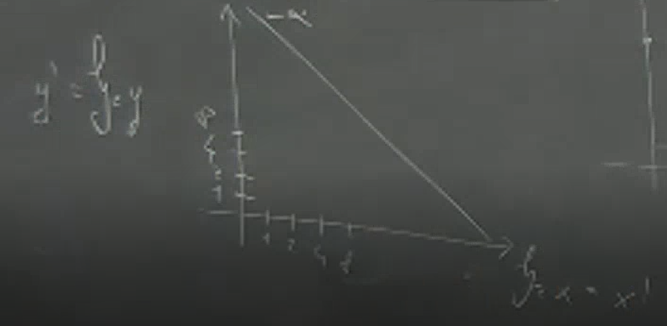
\includegraphics[width=0.75\linewidth]{images/loglog.png}
    \caption{Plot with a log log scale}
    \label{fig:loglog}
\end{figure}
In the real life it doesn't happen that you obtain an exact line, but in the middle you have a lot of points that are on the line and at the borders you have something like a "noise". There was a discussion between researchers at the end they ended saying that this wasn't a power law, but a combination of power laws; in general if you have a large part in the middle that share the line you consider it a power law.
It's amazing how this law it's not true only for \textit{in-links} and \textit{out-links}, but it's true even for \textit{connected components} (x = number of pages and y = number of connected components) even for \textit{strongly connected components} this occurs even in the distribution of the words, obviously the value of $\alpha$ changes.\newline
From this we can immediately notice that we will have a lot of pages whose adjacency list is made by one element because there are a lot of pages with one hyperlink.\newline
\section{Locality}
To exploit the property of locality we sort URLs by reversed domain ("www.di.unipi.it" becomes "it.unipi.di.www") in this way we have that hyperlinks that are similar of the same domain like "di.unipi.it" and "vet.unipi.it" are locally near each other otherwise I will have million of pages between them if I sort without reversing.\newline
This is a very trivial idea, but very efficient in terms of space. For example if the hyperlink "it.unipi.di.www" is at the position \textit{x} the hyperlink "it.unipi.vet.www" is at the position \textit{x+d} where \textit{d} is a small number ($d \approx 1$).\newline
So the adjacency list of the page u contains a set of pages (hyperlinks) that goes from u to them, but since we said that for each hyperlink we assign an id, the id of them (hyperlinks pointed by u) will have a value close to the value of u. Obviously suppose that u=10 then the adjacency list of u can be made by 12,15,5 (even smaller number of u), but for sure the hyperlinks are clustered around u.
\section{Similarity}
Suppose that we have two pages \textit{u}, \textit{v} that are in the same host, this means (according to the sorting of locality) that they are close in the sorted order.\newline
Now let's analyze what "they share many hyperlinks" means: if the adjacency list of u is u=25 $\to$ 3,5,15,20,27,... then v=26 I expect that the adjacency of v looks similar to the adjacency of u.
For example v can be v=26 $\to$ 2,5,15,16,37,....\newline

\section{Web Graph Compression}
The following algorithm that we are going to describe is based on these three properties and it's very effective because it's able to represent a Web Graph using just three bits per edge which is impressive.\newline
First of all we start from having the uncompressed adjacency lists so we have several adjacency lists, we can see an example in the following Figure \ref{fig:uncompressedad}.
\begin{figure}
    \centering
    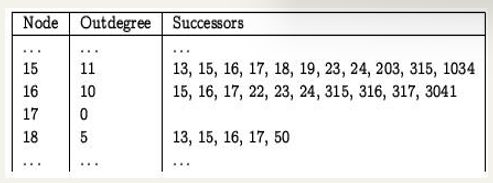
\includegraphics[width=0.75\linewidth]{images/uncompressed.png}
    \caption{Example of uncompressed adjacency list}
    \label{fig:uncompressedad}
\end{figure}
The \textbf{first step} consists of building the \textbf{copy list}, first of all we know that docIDs close share many hyperlinks in particular for every list looks back at most to W previous adjacency lists (usually W is set to 8) we search for the best list to match with. For example if the hyperlink \textit{v=18} we look at 17,16,...,10 and we look for the best list to match, what means "best list"? the one that shares many numbers (hyperlinks), we search for the best copy back.\newline
We call \textbf{reference list} the list that we are looking at that's why we call it "reference". In the following Figure \ref{fig:copylist} we show an example. Usually we partition the nodes in blocks of size W otherwise if I have a lot of references for example v refers to u and u refers to z I'm creating something like a "chain" that it's not efficient.
\begin{figure}
    \centering
    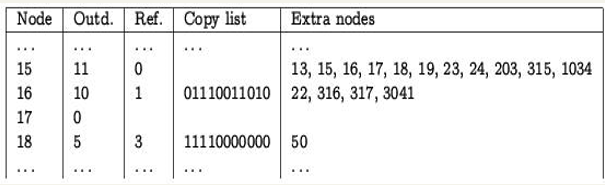
\includegraphics[width=0.75\linewidth]{images/copylist.png}
    \caption{Example of Copy List}
    \label{fig:copylist}
\end{figure}
Here we have \textbf{node} that it tells us the node that we are compressing, \textbf{out degree} that it's the number of the hyperlinks that it has, \textbf{reference} that it's an integer that tells us how back I have to go (the reference list has set this value to 0). Then we have \textbf{copy list} that it's a sequence of bits (0 and 1) that it's created looking at the reference list and setting the bit to 1 if the i-th element of the reference list is present in the adjacency list that we are compressing, 0 otherwise. At the ende we have \textbf{extra nodes} that are the nodes present in the list that we are compressing, but they are not present in the reference list. Notice that the length of the copy list is exactly the out degree of the reference list.\newline
Notice that for the reference list the column copy list is empty and all the nodes are seen as extra nodes.\newline
The \textbf{second step} is the \textbf{copy block} that it's based on the \textbf{RLE} - Run Length Encoding where we build a table that it's similar to the previous one, but we remove the column \textit{copy list} and we add the column \textbf{number of blocks} that it's the number of the blocks equal in the copy list and we have the column \textbf{copy blocks}.\newline
How do we build the copy blocks? We set the first bit to 0 or 1 if the copy list starts with 0 or 1 (we tell to the decompressor how it must start) this is the start bit. Then we write the length of each block - 1 that it's the RLE. 
In the following Figure \ref{fig:copyblock} it has been shown an example.
\begin{figure}
    \centering
    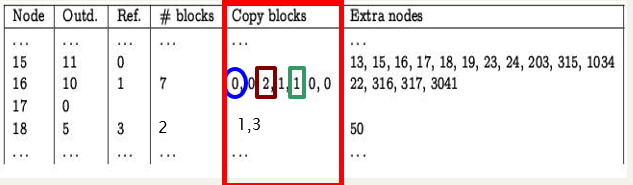
\includegraphics[width=0.75\linewidth]{images/copyblock.png}
    \caption{Example of Copy Block}
    \label{fig:copyblock}
\end{figure}
Notice that even in this case the reference list has undefined the columns copy block and number of block.\newline
For the copy block we use the \textbf{Variable Length Representation of Integers} that allows us to represent integers using few bits for small numbers and high bits for large numbers and that's why to use this technique here because I have small numbers.\newline
There is another \textbf{optimization trick} that tells us to drop the last block because we can compute it knowing the out degree of the reference list.\newline
This algorithm is impressive because as we said before we typically use 3 bits per edge.\newline
Remember that we have extra nodes and we must compress them too and there are several ways to store them, just to give an idea we can use \textit{gap coding} since they are sorted (but there are more efficient solutions).\newline


These tricks that we have seen work perfectly on Web Graph, but in other applications like social networks they don't work because for example the first problem is how do we sort the lists? I can't order lexicographical because I can have friends with names that aren't close to the mine.
\chapter{Locality Sensitive Hashing}
The technique called \textbf{Locality Sensitive Hashing} that we will discuss in the chapter allows us to solve not only problems related to web search, but also in databases or in general in mining problems. In particular this technique allows us to find similar pages and during the crawling we are interested in finding similar pages.\newline
It's an hashing technique that it's sensitive to locality in the sense that if I take two objects that are very similar the technique is able to discover the similarity in an efficient way.\newline
Now let's define the \textbf{Hamming Distance}: given two vectors \textit{p} and \textit{q} with d components, in particular they are binary components $p,q \to {0,1}^d$ we call  \textbf{Hamming distance} between p and q as the number of different bits $D(p,q)=number of different bits$. In few words we align the two vectors and we count how many different bits there are between them.\newline
Let's look at an example and suppose that we have $p=101100$ and $q=111101$ then D(p,q)=2 and d=6 (number of components).\newline
Now let's define what is the \textbf{similarity} between p and q as: 
\begin{equation}
    s(p,q) = \frac{d-D(p,q)}{d}
\end{equation}
From this formula we can see that $d-D(p,q)$ gives us the number of equal bits and therefore if the two vectors are totally equal we have 1 otherwise if they are totally different then their similarity is equal to 0.\newline
It's clear that we have these bounds on D(p,q): $0 <= D(p,q) <= d$ from this we have $0 <= s <= 1$.\newline
This kind of vectors occurs many times in search engine or databases or data mining so our goal is that given a set of some vectors we want to find the subset of them in which the vectors are similar among them.\newline
We can't sort the two vectors because suppose that they have just one different bit at the end it's good because they are near, but if the different bit is at the beginning of them they will be totally far each other even if they are similar. This problem was a big problem and people usually used brute force approach that in big data this obviously it's not affordable up to the point some researchers created a technique very efficient.\newline
They created the Locality Sensitive Hashing: first of all they defined an hash function $h_I$ that it's parameterized by I where $I = set of positions in {1,2,...,d}$ and the cardinality of I is k, |I|=k. So the value of \textbf{$h_I(p)$=projection of p over the positions in I}.\newline
For example if $k=2$ and $I={1,4}$ then $h_I(p)$ are the bits in the positions 1 and 4. Now the question can be \textit{what is I? how do we choose I?} I is chosen \textbf{randomly} so it's a random set.\newline
We apply this for all the vectors so we compute $h_I()$ and then we will have all the projections of the vectors. The key idea is that \textbf{we are transforming the search for small Hamming Distance into a search over equal projected vectors}. In other words instead of computing the Hamming distance between all the vectors to find the most similar I use this technique to search equal projections (because it's simple to check if they are equal, it's just a match).\newline
Now the problem is that how much do we lose with this transformation and how can we control it, in other words are we finding matches that don't exist or we aren't considering matches because the projections are different (false positives and false negatives), but we will discuss about this soon. In general we need to fix the parameter k, we extract k positions from the vectors and we project the vectors. The \textbf{intuition} is that if \textit{the vectors p and q are highly similar I expect that their projections are exactly the same}, but it can happen that when I pick the positions I consider just the different positions (I'm unlucky).\newline
\section{Property: probability that two projections are equal}
We want to compute the probability that two projections are equal so: $P (h_I(p)=h_I(q))$, in other words the probability that two vectors p and q have the same projections for the same set I with cardinality k.\newline
The probability that two positions are equal is \textit{s} so to compute the probability that two projections are equal is this probability that we have just computed k times. so $P (h_I(p)=h_I(q))=s^k$ because all the extraction are independent. Notice that more the two projections are similar higher will be this probability and if I increase the value of k the probability will go to 0. In the following Figure \ref{fig:probham} it has been shown the plot related to the probability.
\begin{figure}
    \centering
    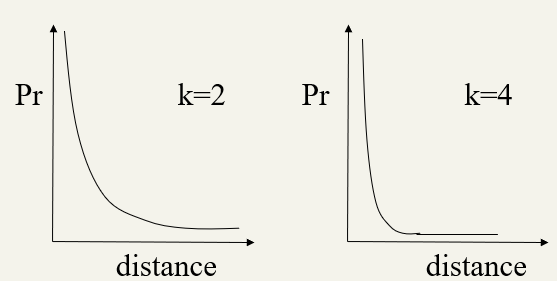
\includegraphics[width=0.75\linewidth]{images/probabilityham.png}
    \caption{Plot where x is (1-s) and y is the probability that two projections are equal.}
    \label{fig:probham}
\end{figure}
It's clear that more we go to the right (the two vectors are different) the lower will be the probability that their projections are equal. Notice that increasing k the function will become \textbf{steeper}, larger k faster the probability goes to 0.
Let's discuss about the problem of false positive and false negative. It's very difficult that I have false positive instead to have false negative depends a lot on the size of k, but it can happen that when I pick the positions I pick all the equal positions and in that case I have a false positive.\newline
Look what happens if I increase k I have that the false positive goes down, but the false negative increases, I need to find a balance between the two cases.\newline
\section{Locality Sensitive Hashing}
Now that we have discussed about the basis and some properties of the projections let's look how this technique works.\newline
The idea is:
\begin{enumerate}
    \item Iterate for \textit{L} times (parameter that we choose on construction) the construction of $I_1$, $I_2$, ..., $I_L$ random set of \textit{k} positions;
    \item We create the \textbf{"fingerprint"} of vector p defined as $g(p)=<h_{I_1}(p), h_{I_2}(p), ..., h_{I_L}(p)>$ where each $h_{I_i}(p)$ is a sequence of k bits (every block is independent to the other);
    \item We declare p similar to q: g(p) $\approx$ g(q) $\iff$ $\exists$ j s.t. $h_{I_j}(p)=h_{I_j}(q)$ at least one of them, I'm not requiring all of them;
\end{enumerate}
In the following picture it is shown an example of Locality Sensitive Hashing (Figure \ref{fig:examplelsh}).
\begin{figure}
    \centering
    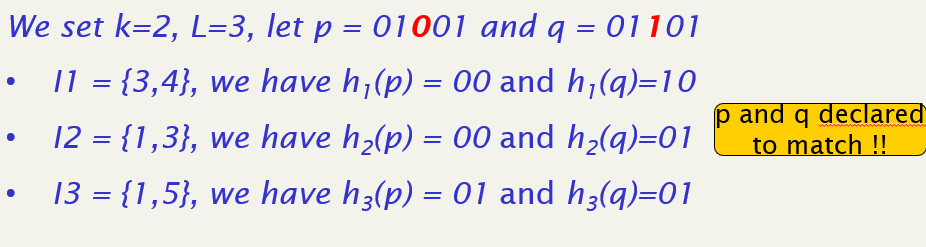
\includegraphics[width=0.75\linewidth]{images/examplelsh.png}
    \caption{Example of Locality Sensitive Hashing}
    \label{fig:examplelsh}
\end{figure}
Someone can ask why are we doing this instead of compare two vectors the answer is that in that case our complexity is O($n^2$), instead with this technique we have a complexity that it's close to sorting complexity O(n*log n).\newline
\section{Probability that two vectors are declared similar}
Now let's have a look to the probability that two vectors, p and q, are declared similar.\newline
Compute the value of this probability:\newline
P(p,q are declared similar)$=$P(g(p) $\approx$ g(q))$=$P($\exists$ j s.t. $h_{I_j}(p)=h_{I_j}(q)$) = 1 - P($\forall$ j s.t. $h_{I_j}(p) \neq h_{I_j}(q)$) = 1 - [P($h_{I_1}(p) \neq h_{I_1}(q)$)$]^L$ = 1 - [1-$s^k]^L$.
So if we have that p and q are equal we find that the probability is equal to 1, 0 otherwise.\newline
If we plot the function obtained we will see that it has the shape shown in the Figure \ref{fig:lshfunction}.
\begin{figure}
    \centering
    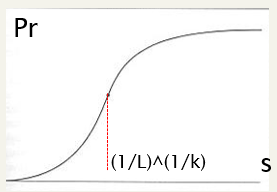
\includegraphics[width=0.75\linewidth]{images/lshfunction.png}
    \caption{Plot of the function where the x is the similarity and the y is the probability that two vectors are declared similar.}
    \label{fig:lshfunction}
\end{figure}
In particular the point where the function change (turning point) is at $(\frac{1}{L})^{\frac{1}{k}}$.
We can't say that this algorithm is always correct because we choose random positions, but in the Web we expect that if two pages are highly similar then this algorithm works in this case and for sure we know that two pages more are similar more my algorithm is correct.\newline
The word "locality" is referring to the geometry of these points in particular this technique has been introduced because in computational geometry there was the problem to find points that were close in the space and there wasn't an efficient algorithm, but thanks to this technique it's now possible.
\section{Locality Sensitive Hashing Algorithm}
There are two versions of this algorithm and first one that we are going to describe is the \textbf{offline version}.
The steps are:
\begin{enumerate}
    \item Fix k, L and extract $I_1$, ..., $I_L$ each $|I_j|=k$;
    \item Compute $g(p_1)$, ..., $g(p_n)$ for all the vectors $p_1$, ..., $p_n$ (this requires just one scan);
    \item For $j=1$ to L: sort g() for all the points according to $h_{I_j}()$; in other words I for each component of g() I sort them so I will do L sorts; it takes O(L*n*log n);
    \item Compute connected components of a graph where the nodes are $p_i$ and the edges are the similarity (similar $p_1$ and $p_2$ means an edge between them); 
\end{enumerate}
We have \textbf{transitivity} property that says if $p_1$ and $p_2$ are similar for $h_{I_1}()$ and $p_2$ and $p_3$ are similar for $h_{I_2}()$ then I say that $p_1$, $p_2$ and $p_3$ are similar.\newline
Whenever I discover that two vectors are similar then I create an edge between them; each sort creates new edges. Notice that when I create the connected components I don't need to create edges for all the matches (if I have that A, B and C are declared similar I can just create two edges $e_1=(A,B)$ and $e_2=(B,C)$ I don't need to create an edge between A and C).\newline
Now look at the second version of the algorithm that it's called \textbf{online version} and in this case you have a query vector q and you want to find all the vectors in your set S which are similar to q.\newline
We use this version in database settings.
The steps are:
\begin{enumerate}
    \item We create L hash tables, one for each projection, $T_1$, ..., $T_L$;
    \item Each hash table has $2^k$ cells that go from 0 to $2^k-1$ because I'm using the projections as a key to access to the table;
    \item For each vector I compute the key (apply projections) and I put the vector in all the Hash Tables;
    \item When I need to do a query I compute the key L times and then I will have the lists of the vectors that are similar;
\end{enumerate}
I do L accesses to the memory and in constant time and I pick a sequence of vectors.\newline
Since we are in a database settings we want to be sure that the values that I picked are equal to my query so for the selected vectors I compute the Hamming Distance having the real result; this is good because I compute it only for few vectors instead of all the vectors;\newline
The \textbf{total cost} is (L + number of checked vectors) and the number of checked vectors are of two kind: the good ones (real similar) and the bad ones (fake similar that according to my mathematics is very low).
\section{LSH vs. K-Means}
In the following section are shown the differences between LSH and K-Means.
\begin{itemize}
    \item \textbf{What about optimality?} \textit{K-Means is locally optimal} vs. \textit{LSH finds correct clusters with high probability};
    \item \textbf{What about the Similarity cost?} \textit{K-Means compares vectors of d components} vs. \textit{LSH compares very short (sketch) vectors};
    \item \textbf{What about the cost per iteration?} \textit{Typically K-Means requires few iterations, each costs K x U x d} vs. \textit{LSH sorts U short item, few scans};
    \item \textbf{What about K?} \textit{You have to iterate K=1, ..., U} vs. \textit{LSH doesn't need to know a prior the number of clusters};
\end{itemize}
Notice that you can apply K-Means over LSH-sketch vectors.\newline
An example of this application can be Trip Adivsor where every element of S is an user and each element of a generic $s_i$ is a restaurant then I can group users with similar tastes; it can be applied even to Netflix suggestions or Football analysis.\newline
\chapter{Document Duplication}
The Web is full of duplicate documents for example there are estimations that 40 \% of the pages are duplicates of others. We can think that some duplications are legitimate like mirror of web pages or content aggregators; on the other hand we can have spam pages or plagiarism and so on.\newline
In general we want to recognize duplicate documents in order to keep our storage low.\newline
We should highlight two kinds of duplicate document detections:
\begin{itemize}
    \item \textbf{Exact duplicate documents} detection;
    \item \textbf{Near duplicate documents} detection that it's more important because they are more frequent; let's think of pages that are equal except for the fact that the only difference is a dynamic content like the date or the users comments;
\end{itemize}
\section{Exact-Duplicate Detection}
We start discussing the first one in particular we are going to see some obvious (slow) techniques and then we will see Karp-Rabin fingerprint.\newline
Let's look at the first naive solution which consist of: given a set of pages we compare per pair all the pages and this computational cost is very high because it takes $n^2*$ \textit{length of the page}.\newline
One immediately improvement that we can do is replacing the web pages with an hash, basically you compute the hash using few words such that it can be stored in a computer register and the hash function you can use the hash that you want. There are some hash functions like \textit{Checksum} (no worst-case collision probability guarantees) and \textit{MD5} (cryptographically-secure string hashes). So first of all if we want to check if two web pages are equal we check the key and if we have a collision then we check the whole page (that happens rarely).\newline
Another improvement that we can do is that now we have \textbf{fingerprints} instead of do $n^2$ comparisons we can sort them and then we will have that equals fingerprints are in the same neighborhood. In this case the computational cost becomes just the cost of sorting and in this particular case we have small integers so we can apply \textit{radical sort} that takes a linear time. Of course first of all you have to pre-process the pages (\textit{offline work}), you do this just once.\newline
\subsection{Karp-Rabin's scheme}
This technique is another technique that allows us to do Exact-Duplicate Detection and it's based on three properties:
\begin{enumerate}
    \item Rolling Hash;
    \item Algebraic Technique;
    \item Efficient;
\end{enumerate}
Now let's have a look in more details to the \textbf{Karp Rabin Fingerprints}: given an m-bit string \textit{A} that it's binary so $A=a_1a_2...a_n$ and $a_i \in \{0,1\}$.
Assume first of all that $a_1=1$ and now fix a universe $U=2^{64}$ where $2^{64}$ is the size of the modern register.\newline
The next step is to choose a \textbf{prime number} $p \in [2, U]$ uniformly at random then we define the Karp-Rabin \textbf{fingerprint} of \textit{A} as $f_p$(A)=A mod p = ($a_1*2^{m-1}+a_2*2^{m-2}+...+a_m*2^0$) mod p.\newline
\textbf{First Property:} it is \textbf{efficient} to compute because you need a shifting and an addition.\newline
\textbf{Second Property:} the \textbf{probability of collisions} is very low. Let's look at the proof $P(f_p(A)=f_p(B)| A \neq B)$ and looking at the definition of Karp Rabin Fingerprints we have that $f_p(A)=f_p(B)$ \textit{A mod p = B mod p} in particular we have that \textit{(A-B) mod p = 0}. From this we can turn our problem into computing:\newline P( p divides A-B)=(\# primes dividing A-B)/(\# primes in [2, U]).\newline
Numerator: let's see at the fundamental theorem of the arithmetic for which each number can be written as the product of several prime numbers. So we have $A-B=p_1^{j1}*p_2^{j2}*...*p_k^{jk}$ for some k and j, we are doing a prime factorization (of course all the $p_i$ are greater or equal than 2).\newline
Now write A-B=C=$c_1*2^{m-1}+c_2*2^{m-2}+...+c_m*2^0$, from this we can obviously infer that $k <= m$. We know that the number of primes that can divide A-B is at most \textit{m}.\newline
Denominator: theorem the number of primes in [2, U] >= $\frac{U}{ln U}$ (for U >= 17).\newline
So let's recall our fraction and we can say that P(p divides A-B) <= $\frac{m}{\frac{U}{ln(U)}}$ that it's equal to $\frac{m*ln(U)}{U}$.\newline
We found that the probability that we have a collision is smaller or equal of the fraction between [m*ln(U)] and (U). From this we see that this probability is very low because typically m is a short value and the $ln(U)=64$ and the denominator is $2^{64}$.\newline
\textbf{Third Property:} it is a \textbf{rolling hash}. It means that you can compute it in just one single step. Suppose that we have a window where you compute the hash of pieces of the document and you have to move this window through the document. Every time you move the window the property that Karp-Rabin fingerprints guarantee is that you haven't to recompute all the fingerprints from scratch (you don't have to do a number of the steps equal to the length of the window), but you have to do just some simple operations in constant time.\newline
Assume you want to check the occurrences of an m-bit pattern p against an n-bit document D where obviously the pattern is much shorter then the length of the document (m $\ll$ n).\newline
\textbf{Algorithm Karp-Rabin}: 
\begin{enumerate}
    \item Compute the fingerprint p $f_p(P)$ (fingerprint of the pattern P choosing randomly a number prime p);
    \item For i=1 to (n-m+1) (end of the document - the length of the pattern)
    \item if fingerprint of p is equal to the fingerprint computed for the window of the document $f_p$(D[i, i+m-1])
    \item then we have a possible match;
\end{enumerate}
The rolling hashing property it's used in the third row of the pseudo code because we are computing in constant time (O(1)) the value of the fingerprint given the window document. The other operations takes O(m) (compute the fingerprint for the pattern p) and O(n) (the number of times that we repeat the for); the overall cost of the algorithm is just O(m+n).\newline
Now see how we can update the fingerprint of the document, we start with the first window D[1,m]=$d_1*2^{m-1}+d_2*2^{m-2}+...+d_m*2^0$ when we move the window by one position we have that the window becomes D[2,m+1]=$d_2*2^{m-1}+d_3*2^{m-2}+...+d_{m+1}*2^0$ basically we shift just one position to the left and we add the next character.\newline
Formally we did: $(D[1,m]-d_1*2^{m-1})*2+d_{m+1}$.\newline
Now we explain why we add 1 in front of the string if we have strings like: "01", "001" or "0001" their representation is equal for all of them and it's "1", but if we add 1 in front of each string then we get "101", "1001", "10001" and all of them are different.\newline
\section{Near-Duplicate Detection}
As we said this problem is very important because near-duplicate pages are more frequent because as we already said two pages can be different just because they have different date or users comments. In 1997 researchers estimated that around 30 \% of web-pages are near-duplicates documents.\newline
\subsection{Shingling}
The first technique that we introduce is called \textbf{shingling} and the idea is to dissect document into \textbf{q-grams} (shingles) in other words a q-gram is a tuple composed by \textit{q} words.\newline
Let's look an example: T={\textit{I live and study in Pisa, ...}} if we set \textit{q=3} the \textit{3-grams} are: \textit{<I live and><live and study><and study in><study in Pisa>...}. Each q-gram is called \textbf{shingle} and the whole technique is called \textbf{Shingling}.\newline
A first thing that we can do is to represent documents by a set of hashes or shingles and more different shingles two documents share more we can say that the two documents are similar. For example if two pages are equal it means that they share all the shingles and their intersection will be the maximum one.\newline
In the following Figure \ref{fig:shingling} it has been shown how this technique works.
\begin{figure}
    \centering
    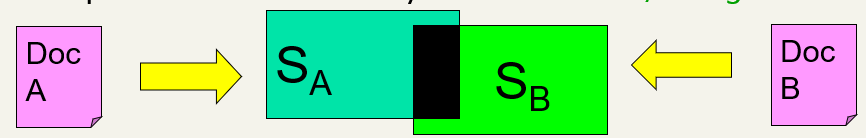
\includegraphics[width=0.75\linewidth]{images/shingling.png}
    \caption{Intersection through shingles between two documents.}
    \label{fig:shingling}
\end{figure}
On the other hand if two documents don't share any shingles then their intersection will be the empty set.\newline
\textbf{How do we choose the value of q?} Typically you choose the value of q between 4 and 8; more in general if you choose an high value of q you are going to do a strictly comparison between the two documents, but on the other hand if there is just one word that it's different then all the shingles overlapped on that word don't match with anyone (so it's very sensitive), we can look this like a trade-off.\newline
\subsection{Jaccard Similarity}
Now we are going to formalize the similarity between two documents counting how many shingles they share thanks to the \textbf{Jaccard similarity}. This let us to assign a value in the range [0, 1] that indicates the similarity between two documents.\newline
We compute the Jaccard similiarity as: $sim(S_A,S_B)=\frac{|S_A \cap S_B|}{|S_A \cup S_B|}$. Where the numerator is the size of the intersection between the shingles of the two documents and the denominator is the size of the union of the shingles of the two documents. We have that the similarity is 1 when they share all the shingles and 0 otherwise.\newline
So in general the idea is to compute the shingles of all the documents and then for each pair of document you compute the similarity using the shingles; in real application you can set a treshold after that two documents are declared near-duplicates for example if you set $j=0.9$.\newline
\textbf{What are the problems of this technique?} The problem is that this set of shingles is very large and they can occupy a lot of space so our ideal technique should have the following features:
\begin{itemize}
    \item \textbf{Storage:} only small sketches of each document (not a full set as we saw);
    \item \textbf{Computation:} the fastest possible;
    \item \textbf{Stream Processing:} once sketch computed the source is unavailable (we can forget about the document and we can just work with sketches);
    \item \textbf{Error Guarantees:} to keep the number of false positives the lowest possible;
\end{itemize}
\subsection{Min-Hashing Technique}
The following technique is used to estimate the Jaccard similarity by using sketches. First of all we start considering the set of shingles for the two documents and applying the Karp-Rabin fingerprints we transform the shingles into numbers that we can map on the universe that goes from 0 to $2^{64}$. After this we apply a permutation to the numbers of each set and this permutation is the same for all the documents of your collection. The simplest permutation that we can do is to compute $a*x+b mod 2^{64}$ which is a permutation that "shuffle" the elements. Obviously if two elements in different documents are equal when I apply the permutation both the elements will be in the same position because the permutation is the same. Now I forget about all the elements of the documents except for the minimum of them and we ask to ourself if the two elements are equal (look at the following Figure \ref{fig:mappingmin}).\newline
\begin{figure}
    \centering
    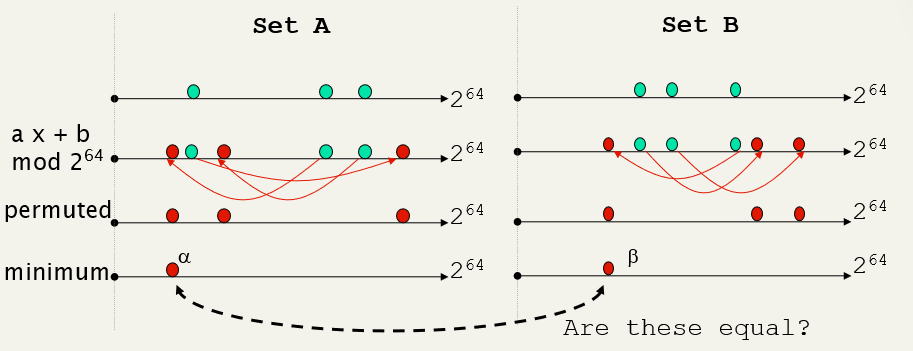
\includegraphics[width=0.75\linewidth]{images/mappingminhash.png}
    \caption{Mapping of the shingles in the universe.}
    \label{fig:mappingmin}
\end{figure}
It turns out the following \textbf{Lemma:} Prob[$\alpha = \beta$] is exactly the Jaccard-sim($S_A$, $S_B$). Now prove this lemma and show why they are similar.\newline
\textbf{Theorem:} Prob[$\alpha = \beta$] = J($S_A$, $S_B$)
\begin{figure}
    \centering
    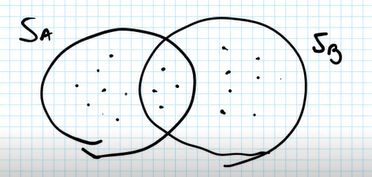
\includegraphics[width=0.75\linewidth]{images/theoremproof.png}
    \caption{Example showed during the proof}
    \label{fig:theoremproof}
\end{figure}
\textbf{Proof:} now we have the two sets with all the shingles like in the Figure \ref{fig:theoremproof} where in the intersection we have the shared shingles. Suppose that after the permutation we have that the minimum of $\pi (S_A)$ ($S_A$ after the permutation) is in the set $\pi (S_A)/\pi (S_B)$ we haven't any possibility that matches with the minimum of $\pi (S_B)$. On the other hand we have the same situation so the probability that $\alpha$ and $\beta$ are equal is 0. The only possible way that two elements $\alpha$ and $\beta$ are equal is only when they belong to the intersection of $S_A$ and $S_B$.\newline
The probability after applying the permutation becomes as the following: we start from the probability that the minimum overall the union of the two sets belong to their intersection. P(min $\pi$($S_A \cup S_B$) = min $\pi$ ($S_A \cap S_B$))=$\frac{|S_A \cap S_B|}{|S_A \cup S_B|}$ = j($S_A$, $S_B$). (At the numerator we have the good cases and at the denominator we have all the cases).\newline
To make our approach more sophisticated we can take more than one permutation having $\pi_1, \pi_2, ..., \pi_k$ where k is around 200. Then we define a \textbf{sketch} of a document as: $SKETCH(D)=[min \pi_1(S_D), min \pi_2(S_D), ..., min \pi_k(S_D)]$. Notice that these sketches are very small because each component of the sketch takes 8 bytes (in total $8 bytes * k=1 Kilo Byte$) against the size of the document that it's much larger.\newline
When we want to compare two sketches we must compare each component pair by pair in an ordered way. After this we count the number of equal components between the two sketches and we divide them by the size of the sketches. We have that: $\frac{equal components}{k}=\frac{k*P(min \pi (S_A)=min \pi (S_B))}{k}=j(S_A,S_B)$. Remember that this is an estimator of Jaccard similarity.\newline
When we have to compare all the documents we can first of all sort by sketches instead of doing $n^2$ comparisons.
\subsection{Cosine distance}
The problem is: given a vector $p \in R_{>= 0}^n$ and p length is $||p||= \sqrt{\sum_{i=1}^n p^2}$. Then we define \textbf{cosine similarity} between two vectors (p and q) as $\cos(\alpha)=\frac{p*q}{||p||*||q||}$ (where p*q is the scalar product).\newline
This is used for example when we compute the score (we will see this later in the course) and for each document we have an array of length n (n is the size of the dictionary) and each entry of the array corresponds to a word of the dictionary that counts the number of occurrences of that word in that specific document. Given some documents we want to compute their similarity through the cosine similarity when we have vectors that show how many times terms appear in their collection, but cosine similarity can be applied to all the kinds of vectors.\newline
Look at this feature: Cosine similarity ranges between 0 and 1, in particular it's 0 when the angle between p and q is 90 degrees instead it is 1 when the angle between p and q is 0 degrees; this means that more the two vectors are close each other more the cosine similarity goes to 1.\newline
Notice that we could have taught at other types of similarity for example the distance between them, but the problem that we can have is if they are close each other, but one of them is very long then they will be declared as non-similar because the distance is very sensitive.\newline
Now see how \textbf{sketching for cosine similarity} works (\textbf{it estimate the cosine similarity}):
\begin{enumerate}
    \item Extract k random vectors uniformly at random $r_1,r_2,...,r_k \in R^n$ (all of them from the same vector space);
    \item Map a vector (document) $p \in R^n$ to a smaller vector (sketch) with components $\{-1,+1\}^k$ (vector of length k where the components are -1 or +1) where obviously k is much smaller of n;
    \item To make this sketch we create SKETCH(p)=[sign(p*$r_1$), sign(p*$r_2$),...,sign(p*$r_k$)] (where p*$r_i$ is the dot product);
\end{enumerate}
From a geometrical point of view it happens that we draw the vector p and the vector $r_i$ then we draw a perpendicular line to $r_i$ and in other words what we do is that we choose +1 if p is in the same hyperplane of $r_i$ or -1 if p is in the other hyperplane of $r_i$. \textbf{Why this happens?} It comes from the formula of the cosine similarity in particular if we multiply both the sides by (||p||*||q||) we get $p*q=||p||*||q||*cos(\alpha)$ and notice that ||p|| and ||q|| are length and this means that they are clearly >= 0 so it means that $\cos (\alpha)$ gives us the sign of the dot product where $\alpha$ goes from 0 to $\pi$ (180 degrees). So if the $sign(p*q)=+1$ it means that the $\cos (\alpha) is >= 0$ and the cosine is greater than 0 when the angle $\alpha$ is between [0, $\frac{\pi}{2}$] (which is 90 degrees, in particular if the angle is 90 degree the cosine is 0). Otherwise if we have that $sign(p*q)=-1$ it means that the $\cos (\alpha) < 0$ and this happens when the angle is between [$\frac{\pi}{2}$, $\pi$] (which is between 90 degrees and 180 degrees).\newline
\textbf{Lemma:} $P(h_r(p)=h_r(q))=1-\frac{\alpha}{\pi}$ where $h_r(p)$ is an element of the sketch of the vector p. This formula is important because thanks to the sketching we can get an estimation of the angle between the two vectors.\newline
Suppose that we want to compute the cosine similarity between two vectors and instead of computing it with all their components we create the sketches that are smaller (length k) and each element has value -1 or +1. To compute the similarity I consider the number of equal components divided by k (/k). The number of equal components can be seen as $k*P(h_r(p)=h_r(q))$/k = 1- $\frac{\alpha}{\pi}$ so I can estimate their "closeness" because I created a bias estimator of the angle of the two vectors. Once I computed the estimated value of $\alpha$ I can compute the cosine $\cos (\alpha)$ and you put a treshold to check if you can declare the two vectors similar or not. It's good because I compute the cosine similarity on small vectors.\newline
\textbf{Proof:} We start from the probability that two element of the sketches are different so we have: $P(h_r(p) \neq h_r(q))$ = P(sign(p*r) $\neq$ sign (q*r)). This happen when the hyperplane perpendicular to r divides the two vectors and one of them will have value +1 and the other one will have value -1 like in the Figure \ref{fig:proofpp}.
\begin{figure}
    \centering
    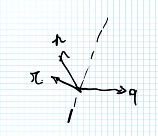
\includegraphics[width=0.75\linewidth]{images/proofpp.png}
    \caption{Vectors p and q separated by the hyperplane.}
    \label{fig:proofpp}
\end{figure}
So continuing we have P(sign(p*r) $\neq$ sign (q*r)) = P(hyperplane defined by r falls between p and q)= number of good cases / number of all the cases = $\frac{\alpha}{\pi}$ (we can choose from $\pi$ hyperplanes and the good cases are $\alpha$). Since we are computing the other probability that's why we take 1-$\frac{\alpha}{\pi}$ = P($h_r(p) \neq h_r(q)$).
\subsection{Time Complexity}
In this section we are going to analyze the time complexity of finding near duplicates in a collection of n documents.
\begin{itemize}
    \item \textbf{Naive solution:} compare all the documents per-wise and we get \textbf{O($n^2$*l)} (where l is the document length) and in this case we can use Jaccard similarity or Cosine similarity;
    \item \textbf{Sketching:}(for cos-similarity where we pick random hyperplanes or for Jaccard Similarity using min-hashing) to use this technique we need to compute all the sketches this costs \textbf{O(n*l)} (pre-processing sketches) + $O(n^2*s)$ where s is the length of the sketch and this is the cost of pairwise comparing the sketches;
    \item \textbf{Sketching + Clustering:} the time complexity is O(n*l) that it's the pre-processing sketches time + the time needed to compute the clusters for example with K-Means we have O(K*n*s*i) where K is the number of clusters and i is the number of iterations (typically few, but we have to consider it); here the problem is to set the value of k so we will spend time to tune K;
    \item \textbf{Sketching + LSH:} the cost is O(n*l) pre-processing sketches + O(L*sort(n)) where L is the number of LSH projections; the sort cost can be O(n*log n) if the n documents fit in the internal memory and they are large otherwise if they are small integers we can use radical sort that take O(n) and at the end if we use external memory the cost will be O($\frac{N}{B}*log_{\frac{M}{B}}\frac{N}{M}$)
\end{itemize}
\chapter{Index Construction}
In this chapter we are going to discuss the construction of the index. We can start with an example and let's suppose that we receive as input the following three documents:
\begin{enumerate}
    \item Caesar likes Brutus;
    \item Caesar likes Calpurnia;
    \item Brutus kills Caesar;
\end{enumerate}
The first time our dictionary will be just an empty set $D=\{\}$ and after that we receive the first document our dictionary becomes $D=\{caesar->[1], likes->[1], brutus->[1]\}$ in the next documents for each words we will check if there is already an occurrence of the word if there wasn't we add the new word. At the end our dictionary will be D=\{caesar->[1,2,3], likes->[1,2], brutus->[2,3], calpurnia->[2], kills->[3]\}. I go on until there is space because our dictionary will be composed of a set of words and for each of them I will have a large number of docIDs. Our goal is to have a fast access to the dictionary and whenever we have to add a document to a posting list we can just append it at the end.\newline
\section{SPIMI}
In this section we are going to see what is \textbf{SPIMI} that stands for \textbf{Single-pass in-memory indexing}. With this technique the key idea is to generate separate dictionaries for each block of documents and then to accumulate postings in lists as they occur in each block of documents.\newline
The algorithm is shown in the following Figure \ref{fig:spiminvert}.
\begin{figure}
    \centering
    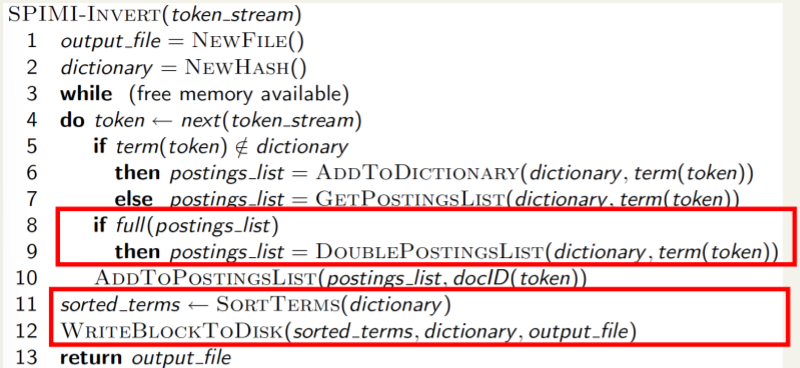
\includegraphics[width=0.75\linewidth]{images/spimiinvert.png}
    \caption{Pseudo code SPIMI-Invert}
    \label{fig:spiminvert}
\end{figure}
I don't have any idea about the size of my dictionary because at the beginning the size is small, but at each iteration I'm adding words and elements to the posting lists. When I start I allocate some space for each term list, but then it can happen that the space I had allocated is full so I need to re-allocate the space of the list.\newline
In the following example it has been shown what happens when we apply SPIMI Figure \ref{fig:spimiex}.
\begin{figure}
    \centering
    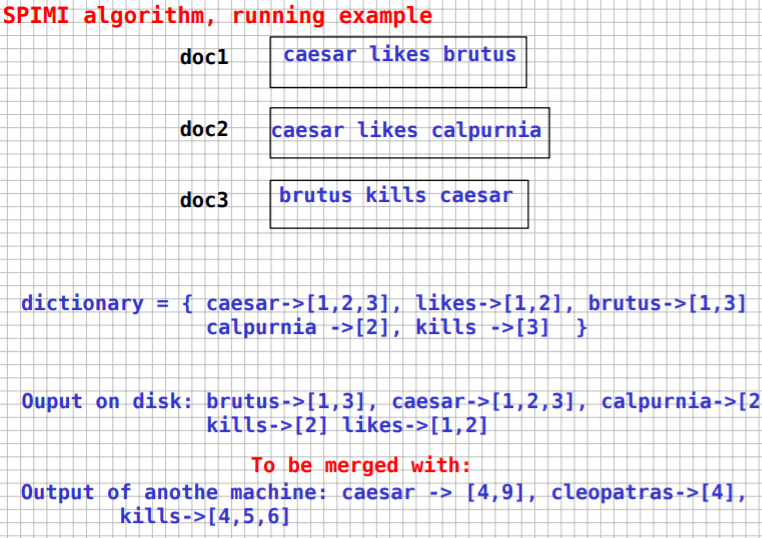
\includegraphics[width=0.75\linewidth]{images/spimiexample.png}
    \caption{Running Example of SPIMI algorithm}
    \label{fig:spimiex}
\end{figure}
We sort the lists because when we have to merge the dictionary of a block of documents with another dictionary that it comes from another machine it's more easy to do it.\newline
There are some issue that we need to address:
\begin{itemize}
    \item How do we find in the dictionary? (time issue);
    \item How do we add to dictionary + posting? (space issue);
    \item How do we choose the postings' size? (doubling);
    \item How do we choose the dictionary size? (in-memory issue);
\end{itemize}
Some issues that we have are: assigning termID, creating pairs <termID, docID> and sorting pairs by TermID (this is a stable sort).\newline
After we have done the processing of various blocks of documents then the next step is to do the merging. We can look at the merging as a merge of sorted pairs.\newline
My goal is to create a single index and to do this I need to take the lists of different sets of documents and create a single one. The merge of different inverted list will be a single inverted list with all the terms that are in at least one block. If a term appears only in one block in the final list it will be unchanged otherwise if it appear in more block then in the final list we will have to concatenate the postings lists.\newline
\section{Multi-way Merge-Sort}
To solve this \textit{huge merging task} we need a sorting that it's disk based and to merge files there is a well-known technique that it's called \textbf{multi-way merge-sort}.\newline
Let's understand better how this merging works, suppose that we have a certain number of blocks of data, each of them is already sorted and I just want to merge them in a unique sorted file that contains all the data. When I read data from a disk there is a fundamental parameter that it's B and it's the \textbf{disk page size} (I can read at most B items for each file). The first thing that I do is to take one page for input file and if I'm lucky all these pages fit in the memory. Now that I have these pages for each of them I take the minimum and I put it in the final output final and I proceed in this way until I finish all the data in these pages. It can happen that during my process I finish all the data of one page so if this happens I just need to do to the corresponding input file and take the next block. I am lucky if I am able to do this in just a single pass, what means to be lucky? it means that the number of pages I'm working with (which is equal to the number of input files) is such all of them can fit in the memory at the same time (it's shown an example in the following Figure \ref{fig:singlestep}).\newline
\begin{figure}
    \centering
    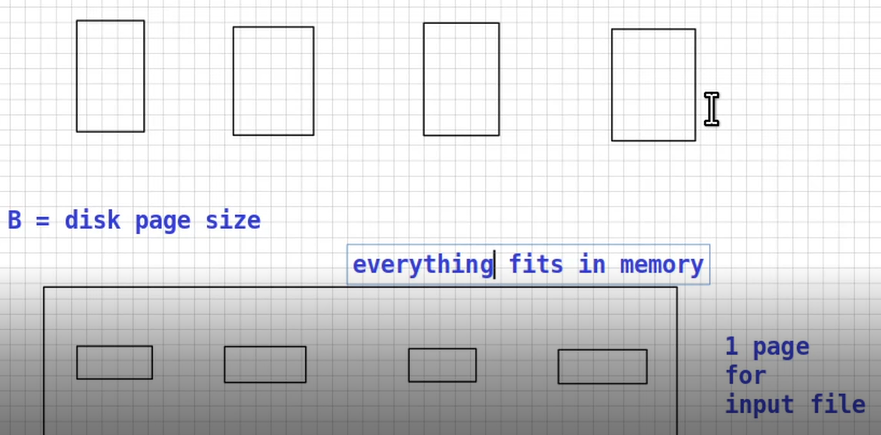
\includegraphics[width=0.75\linewidth]{images/singlestep.png}
    \caption{Example of MWMS when all the pages fit in memory.}
    \label{fig:singlestep}
\end{figure}
In real application it never happens that all the pages fit in memory because we have million of them so we need multiple steps to do this job. Let's look at this case.\newline
We can sort in memory up to M items (our memory is M), and therefore this gives us N/M sorted block that have to be merged. For the merging we are limited by the size of the memory because in the merging we read one block for each file that has to be merged and then we do the merging with all the files. We are able to merge simultaneously a number of files X= M/B (for example if the memory is 1GB and the block size is 10MB then we can store simultaneously only 100 files because for each file we need to load a page of size B). This number X doesn't depend on the size of the files to be merged because this limit depends only on the size of the page of the disk and on the size of the memory.\newline
The problem is: if the blocks to be merged (N/M) are <= X then we are done in one step; otherwise if N/M > X in the first round we take X files of size N/M and merge them into a new file of size X*(N/M); in the second round we take X files of size X*(N/M) and merge them into a new file of size $X^2*(N/M)$; if this is not enough we do a third round, we proceed until we don't finish all the files to merge (proceed until $X^i*(N/M)>N$). In the following Figure \ref{fig:multistep} we show a slide.\newline
\begin{figure}
    \centering
    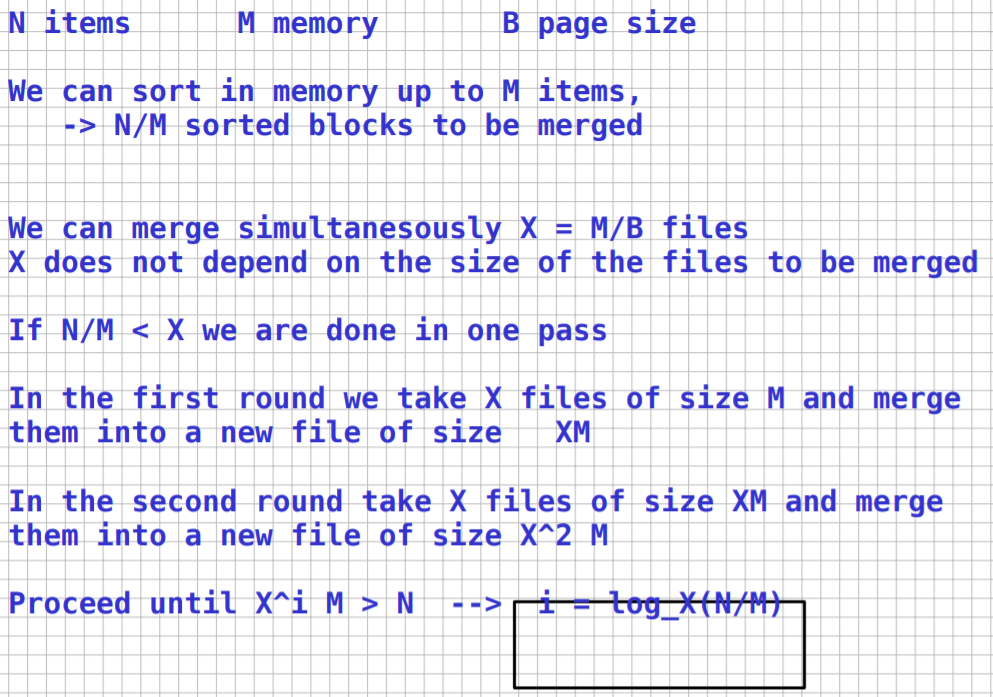
\includegraphics[width=0.75\linewidth]{images/multistep.png}
    \caption{Slide taken from the lecture that shows Multi-Way Merge Sort.}
    \label{fig:multistep}
\end{figure}
The \textbf{cost} of \textbf{Multi-way Merge-Sort} are:
\begin{itemize}
    \item Number of passes = $log_x N/M \approx log_{M/B} (N/M)$;
    \item Total I/O-cost is $\Theta ((N/B)log_{M/B} N/M)$ I/Os (it's interesting look at the role of N in this formula because it will be the largest value and it appear as linear and logarithmic);
\end{itemize}
After this algorithm we will have an unique merged file which for our application is an inverted list for all the documents.\newline
In practice we use this technique when our collection of documents is big, but not very very big. In that case instead we use Distributed Indexing.
\section{Distributed Indexing}
For web-scale indexing you can't do this on a single machine, but you must use a distributed computing cluster of PCs. Individual machines are not the best choice because they are fault-prone for example they can be broken or they can stop working for this reason we need a robust mechanism with several machines.\newline
The \textbf{Distributed indexing} works as follow:
\begin{itemize}
    \item Maintain a master machine directing the indexing job that it's considered "safe"; it's used a mechanism called \textbf{Map Reduce} that does complex tasks on a distributed system; there is a weak point that it's the master machine that works always and shouldn't shutdown;
    \item Break up indexing into sets of (parallel) tasks;
    \item Master machine assigns tasks to idle machines;
    \item Other machines can play many roles during the computation;
\end{itemize}
To build our index we need to do parallel tasks and in this case there are two natural case to break the document collection:
\begin{itemize}
    \item \textbf{Term-based partition:} where one machine handles a sub-range of terms; (for example one machine is in charge to manage all the words that start with the letter 'b' such that the machine knows all the documents that contain a subset of terms); look at Figure \ref{fig:doctermbased};
    \item \textbf{Doc-based partition:} where one machine handles a sub-range of documents; (one machine will see only a fraction of the documents, but that machine will have all the terms that are contained in the fraction of documents); look at Figure \ref{fig:doctermbased};
\end{itemize}
\begin{figure}
    \centering
    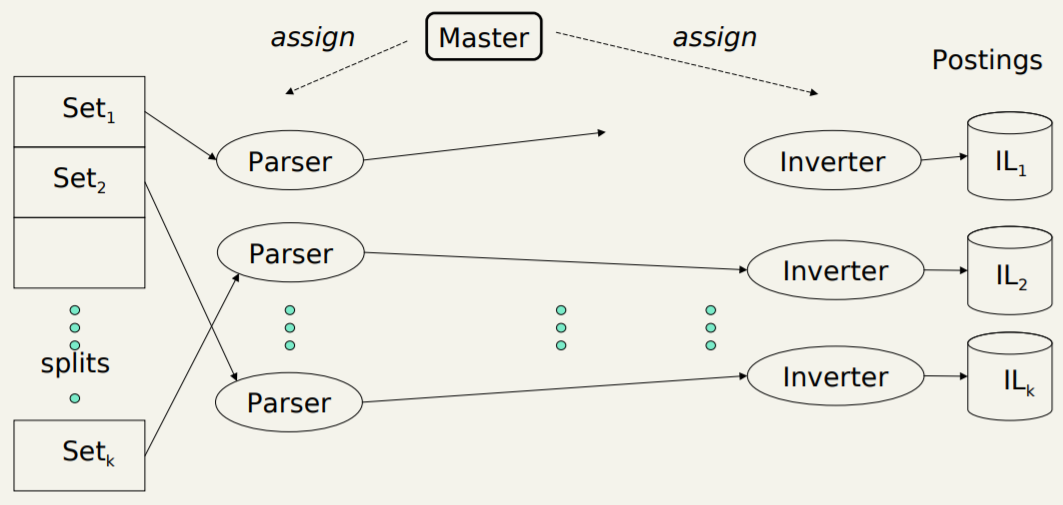
\includegraphics[width=0.75\linewidth]{images/docbasedpartition.png}
    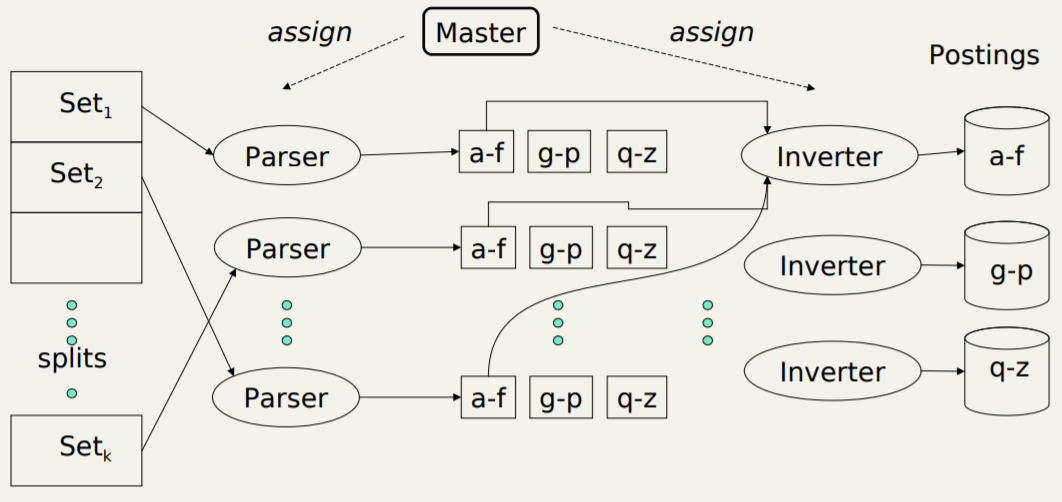
\includegraphics[width=0.75\linewidth]{images/termbased.png}
    \caption{Structure of the Doc-Based Partition above and Term-Based Partition below.}
    \label{fig:doctermbased}
\end{figure}
Looking at the picture \ref{fig:doctermbased} we have on the left sets of documents. In general if we look at the Doc-Based Partition we have that each query-term goes to all the machines instead with the Term-Based Partition we have that each query-term goes to one machine.\newline
When we have to build a structure that it's term-based partitioned it's more complex because we have a sets of documents that are assigned to parser and each of them will produce the complete index for that set of documents that it's already partitioned for the range of terms such that each range will be assigned to the inverter that will be "specialised" on that specific set of terms.\newline
Notice that: the same machine can act either as Parser either as Inverter or if a machine breaks then the master must re-assign the work to another machine.
As we already said there is \textbf{Map Reduce} that it's a robust and conceptually simple framework for distributed computing without having to write code for the distribution part.\newline
Google indexing system consists of a number of phases, each implemented in Map Reduce.
\section{Dynamic Indexing}
Up to this moment we have assumed \textbf{static} collections, but more frequently occurs that documents come in over time or are deleted and modified (let's think of Twitter). This means that postings updates for terms already in dictionary and new terms are added/deleted to/from the dictionary.\newline
The simplest approach to address this problem is to maintain a "big" main index and new documents go into "small" auxiliary index and when we need to do a search we do it across both the indexes and merge the results.\newline
When we need to do some deletions we can do invalidation bit-vector for deleted documents and filter search results by the invalidation bit-vector. At the end we can periodically re-index into one main index.\newline
There are many issues with this approach the biggest one are the poor performance (in particular the merging of the small index with the main one), but luckily there is a good technique to manage dynamic documents that it's called \textbf{Logarithmic Merge}.
In this case where we have Auxiliary and main index we have that each text participates to at most (C/M) merges because we have one merge of the two indexes (small and large) every M-size document insertions (the toal cost is C*(C/M).\newline
\subsection{Logarithmic Merge}
The Logarithmic Merge is a good technique to address the problem of Dynamic Indexing. It maintains a series of indexes, each twice as large as the previous one: M, 2*M, $2^2*M$ and so on. We keep a small index (Z) in the memory (of size M).\newline
Assume that our memory is M and when the memory is full I write the index to the disk so I will have an index of size M. Now my memory is empty so the memory can now handle new documents , but when I have reached size M I have to store again another index of size M on the disk. The idea now is that if in the disk I have another index of the same size I merge them so in this case I will have just one index of size 2M and I continue on this way obtaining M, 2M, 4M, 8M, 16M and so on.\newline
Here it has been shown how the structure looks Figure \ref{fig:logmerge}.
\begin{figure}
    \centering
    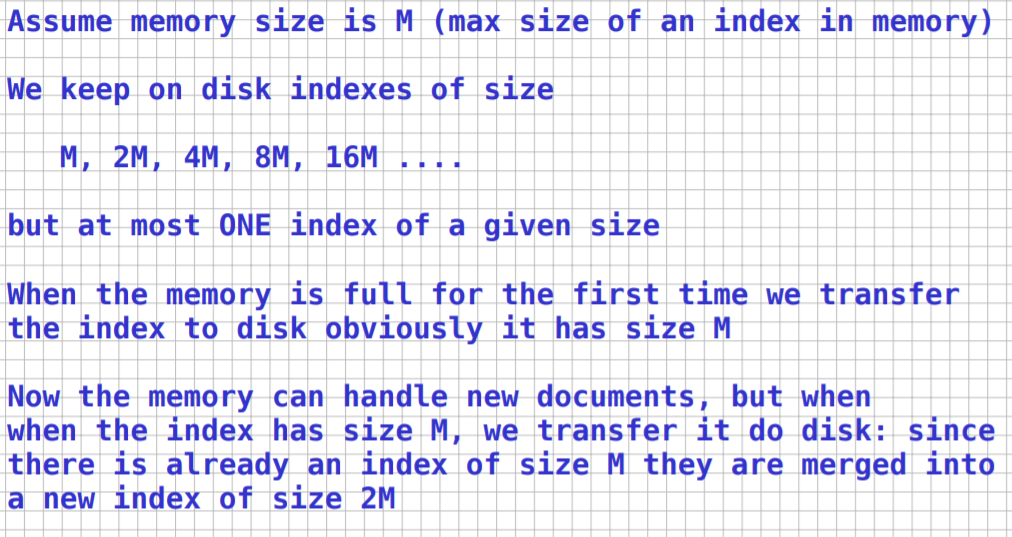
\includegraphics[width=0.75\linewidth]{images/logmerge1.png}
    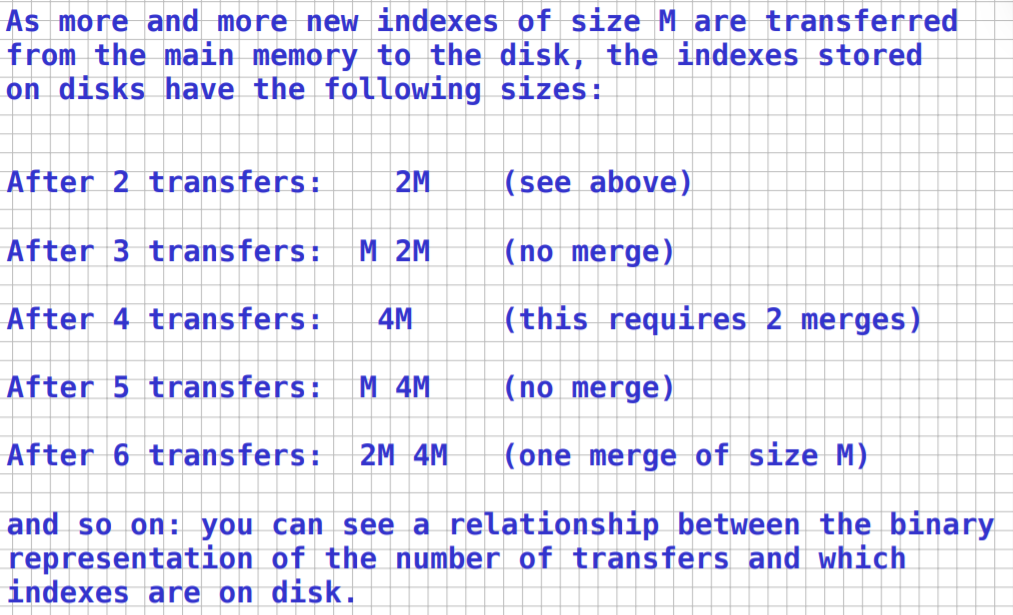
\includegraphics[width=0.75\linewidth]{images/logmerge2.png}
    \caption{How Logarithmic Merge works.}
    \label{fig:logmerge}
\end{figure}
It looks that doing in this way we waste a lot of time, but it's not bad this technique. Let's start saying that for example when we have the index of size 32M it means that each document of this index has been merged 5 times (at size 2, 4, 8, 16, 32). So the number of times that a document has been merged is given by the logarithm in base M of the index ($log_2 (32)=5$). Each text participates to no more than log(C/M) (where C is the total collection size) merges because at each merge the text moves to a next index and they are at most log(C/M). After log(C/M) merges, it will be in a group of size $2^{(log(C/M))}*M=(C/M)*M=C$. Since this is the largest possible size, no text will undergo more than log(C/M) merges.\newline
Now let's have a look at the total cost that it's $C*log(C/M)$.
\chapter{Document Parsing}
In this chapter we do one step back and we analyze some concepts that we haven't studied in details in particular we will see the process that goes from the document to the terms that will be part of our index (the process from documents to indexing).\newline
In the following Figure \ref{fig:invertedindexconstruction} it's shown the process.
\begin{figure}
    \centering
    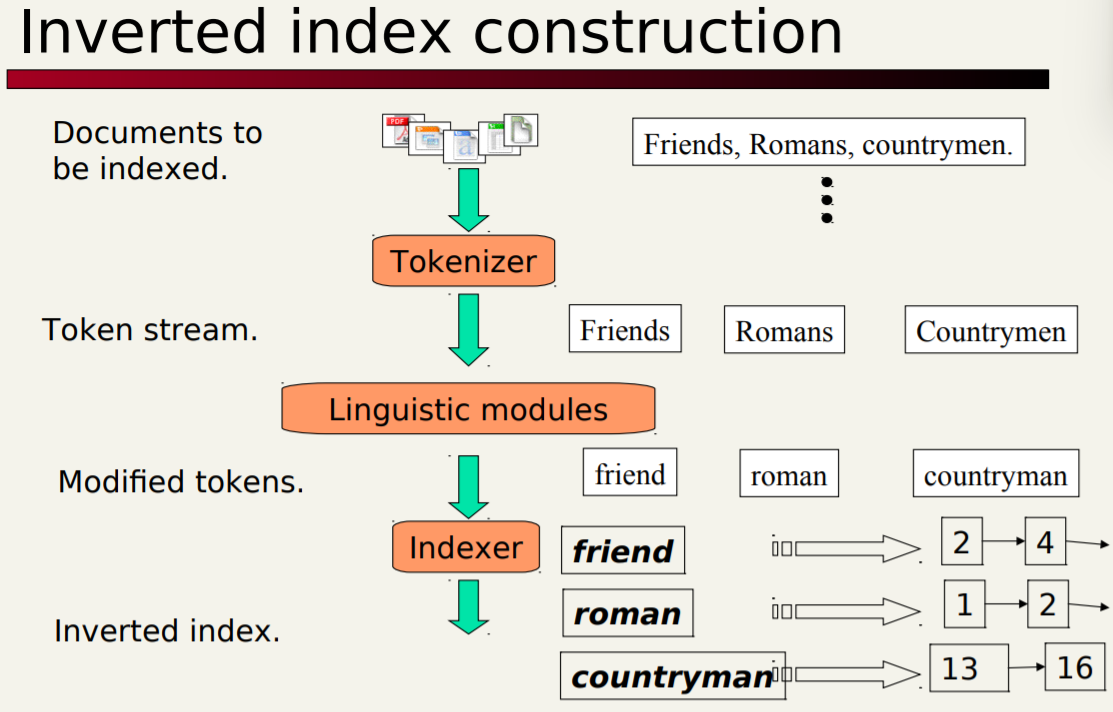
\includegraphics[width=0.75\linewidth]{images/invertedindexconstruction.png}
    \caption{Structure of the construction of the inverted index.}
    \label{fig:invertedindexconstruction}
\end{figure}
At first we have the documents to be indexed and the first step that is done by \textbf{Tokenizer} where we build a \textbf{Token Stream} (in this process we remove the notations like "," or "."). The second step goes from the Token Stream to the \textbf{Modified Tokens} thanks to the \textbf{Linguistic Modules} where we modify tokens according to some linguistic rules (for example if we have "Friends" and "friends" they are equal so we remove capitalization from the words or we normalize them removing the "-s" for the plural). In the last step we go from the Modified Tokens to the \textbf{Inverted Index} thanks to the \textbf{Indexer}.\newline
From a pratical point of view if my query is "friend roman countryman" the output pages will be pages where for example appear "Friends" or "Romans" or "Rome" (with capitalization and plural form), this shows us the concept described above.\newline
The first step to solve this problem is \textbf{Parsing a document} where we need to recognize some features like:
\begin{itemize}
    \item What format is it in? pdf, word, excel or html?
    \item What language is it in?
    \item What character set is in use?
\end{itemize}
Each of these problem is a \textbf{classification problem}, but in practice these are often solved heuristically without using complex classification structures.\newline
Once that we have taken the documents and extracted the text we have to do the \textbf{Tokenization} where in input we have a sequence of words and in output we want tokens. In this phase we need to remove from the text the punctuation and even the conjunctions (we will see later why we do this).\newline
How do we define a token? A \textbf{token} is just an instance of a sequence of characters. Each token is a candidate for an index entry after further processing.\newline
The problem of Tokenization is not so simple because there are many cases where we have problems to decide if two words are one token or two for example:
\begin{itemize}
    \item Barack Obama: is it one token or two?
    \item San Francisco: is it one token or two?
    \item Hewlett-Packard: is it one token or two?
    \item B-52, C++ (acronyms): is it one token or more?
    \item Numbers: do we need to keep them? dates probably yes 24-5-2010 (is it one token or more);
    \item 192.168.0.1 (IP address): is it one token or more?
\end{itemize}
This means that we can't just consider each word independently because there are a lot of words that are composed by two or more of them. A token sometimes (like above) should be a pair of words not just one word (if we split the term we are losing the meaning of that words).\newline
An example related to how complex is when we are doing this process if when your query is "san paolo" and the results are most of them "SanPaolo Bank", but you have other results like "Sao Paulo Brazil".\newline
As we said before the conjunctions are removed from the output they are not written as tokens there is a category of word that we ignore \textbf{Stop Words}: we exclude from the dictionary the most common words. The intuition is that they have little semantic content like "the", "a", "an", "and", "to", "be"; they are a lot around 30 \% of postings for top 30 words so they are very expensive to store them and they don't help when we search something. Notice that there are some exceptions for them for example when we are finding a book or a movie (phrases queries) where in that case you need them because every word is important for example "To be or not to be" we need exactly that words.\newline
Nowadays usually people keep stop words because using good compression techniques it means that the space for including stop words in a system is very small. There are even good query optimization techniques where you pay little at query time for including stop words.\newline
There is another operation that we usually do is \textbf{Normalization} to terms. What does it mean? We need to "normalize" terms in indexed text and query words into the same form because for example we want to match "U.S.A" and "USA". We most commonly implicitly define equivalence classes of terms doing some operations like \textit{deleting periods} to form a term ("U.S.A." becomes "USA") or \textit{deleting hyphens} to form a term("anti-discriminatory" becomes "antidiscriminatory"), but can we do always these operations? No because suppose that we have "C.A.T" if we apply deleting periods operation we get "cat" and this is totally wrong since "C.A.T" it's a brand that sells tools. Most of these problems are solved manually once a time because there isn't a general rule to solve them.\newline
The next operation of normalization is \textbf{Case Folding} where we reduce all letters to lower case, but can we have some exception ("Bush" vs "bush" where the first one is a person and the second one not)? Often it's better to lower case everything, since users will use lowercase regardless of correct capitalization (users are lazy).
Another problem that we are going to analyze is the problem of synonyms \textbf{Thesauri} where we handle synonyms and homonyms by hand-constructed equivalence classes for example we have that "car"="automobile" or "color"="colour" and so on. We have to decide a canonical form that can be: a composition of the terms like "car-automobile" and when the document contains "automobile" we index it under the equivalence-class term "car-automobile" and vice-versa or we can expand a query and when the query contains "automobile" we look under "car" as well. If we are dealing with homonyms we have the same term, but with different meanings and for example we can have two different postings lists for the two meaning, but this requires an analysis of the sentence to understand the meaning of the context.\newline
The next process that we are going to analyze is the \textbf{Stemming} in which we reduce terms to their "roots" before indexing. "Stemming" suggest a crude affix chopping for example if we have "automate(s)", "automatic" and "automation" all it's reduced to "automat" (it's not trivial to solve this problem and it's language dependent). Luckily there is the Porter's algorithm that it's able to do this kind of operation for many languages.\newline
Something that it's related to stemming, but it's more sophisticated is the \textbf{Lemmatization} (it comes from "lemma" which is the word under which a term appear in the vocabulary) where we reduce inflectional/variant forms to base form for example if we have "am", "are" or "is" they become "be", the same for "car", "cars", "car's" or "cars'" that becomes "car". This is clearly more complex (it requires some knowledge about the language) then stemming because there we are just removing characters without changing the word too much, but in this case we change a lot.\newline
At the end we can clearly say that most of the above features embody (\textit{"incarnare"}) transformations that are \textbf{language-specific} and often \textbf{application-specific}. In the years have been done several experiments to understand if stemming can help and it has been shown that for example in English it gives as output very mixed results so it helps recall for some queries but harms precision on others because for example if we have "operative", "operational" and "operations" they become "oper" (they have different meanings); for other languages it turns to be definitely useful like Spanish, German and Finnish (it gains 30 \% performance for Finnish).\newline
Now let's have a detailed look at this table in the following Figure \ref{fig:tableindex} where we see the size of the dictionary for three different cases the first one is composed just by terms, the second one is composed by non-positional postings and the last one is composed by positional postings (just positional indexes where we save even the positions where the term occurs in the document and clearly this index is much larger then the others). It can be seen how using these techniques the size of the dictionary decreases a lot.
\begin{figure}
    \centering
    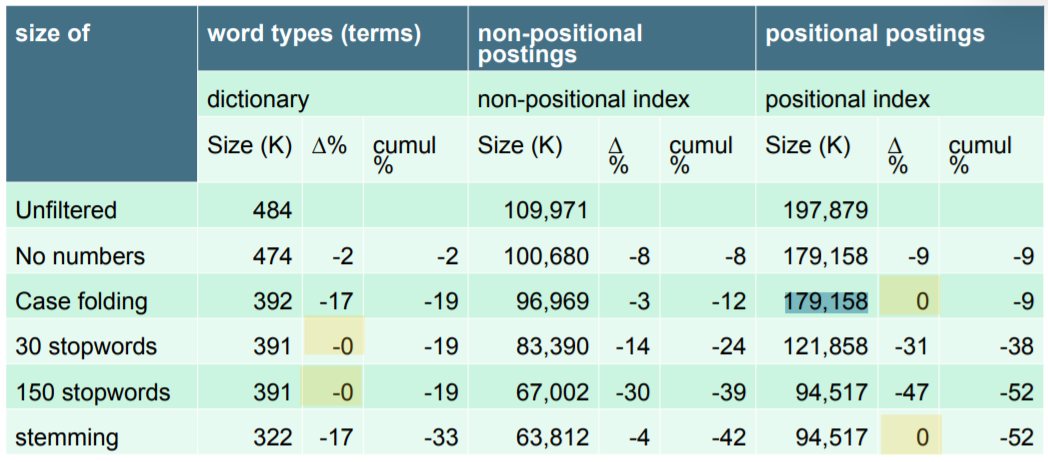
\includegraphics[width=0.75\linewidth]{images/tableindex.png}
    \caption{Table with index parameters.}
    \label{fig:tableindex}
\end{figure}
\section{Statistical Properties of texts}
In this section we are going to discuss some statistical properties of texts. It has been seen that the tokens are not distributed uniformly, but they follow the empirical \textbf{Zipf Law} (that it's true for several languages) for which:
\begin{itemize}
    \item Few tokens are very frequent;
    \item A middle sized set has medium frequency;
    \item Many are rare;
\end{itemize}
In detail the Zipf Law says that the k-th most frequent token has frequency f(k) approximately 1/k; equivalently the product of the frequent f(k) of a token and its rank k is a constant. So we have k*f(k)=c where c is a constant that it's equal to f(k)=c/k. In other words the first most frequent token appears c times and the second most frequent token appears c/2 times and the third most frequent token appear c/3 times and so on.\newline
There is also a generalized versione \textbf{General Law} where we have $f(k)=c/k^s$ and $s \in [1.5,2]$. This is an empirical law and it's not exactly respected in all the languages in particular is a good fit for the tokens in the middle range.
In the following Figure \ref{fig:zipfcurve} it has been shown how the Zipf Curve looks like and the x is the rank of a word so smaller is the value it means it's the most frequent word and the y is the frequency of that token.
\begin{figure}
    \centering
    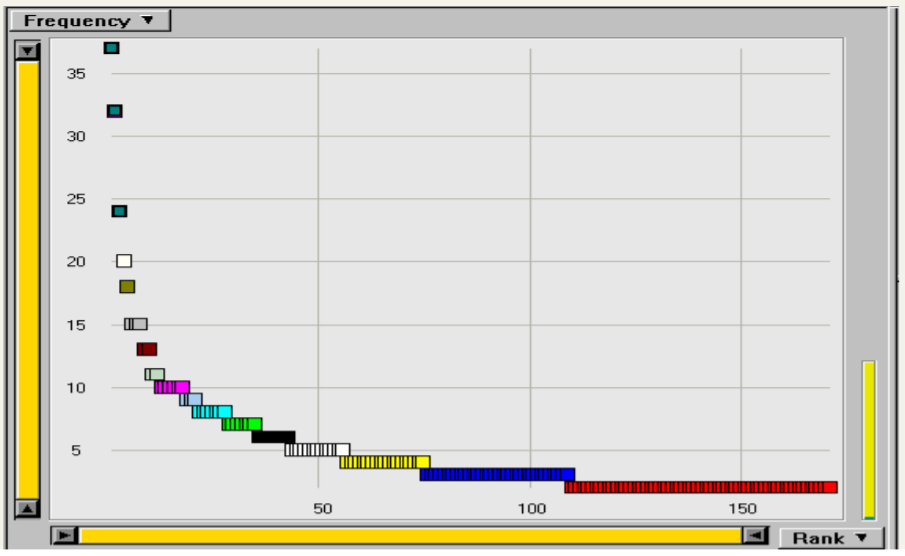
\includegraphics[width=0.75\linewidth]{images/zipfcurve.png}
    \caption{Plot of the Zipf Curve.}
    \label{fig:zipfcurve}
\end{figure}
From the previous Figure \ref{fig:zipfcurve} it's not so clear the law that's why we need a log log plot to see the law. So starting from $f(k)=c/k^s$ we got $log(f(k))=log(c)-s*log(k)$ and if we plot log(f(k)) vs log(k) we get y=log(c)-s*x that it's a line with slope -s.
In the following Figure \ref{fig:loglogzipflaw} it has been show how the log log plot looks like.
\begin{figure}
    \centering
    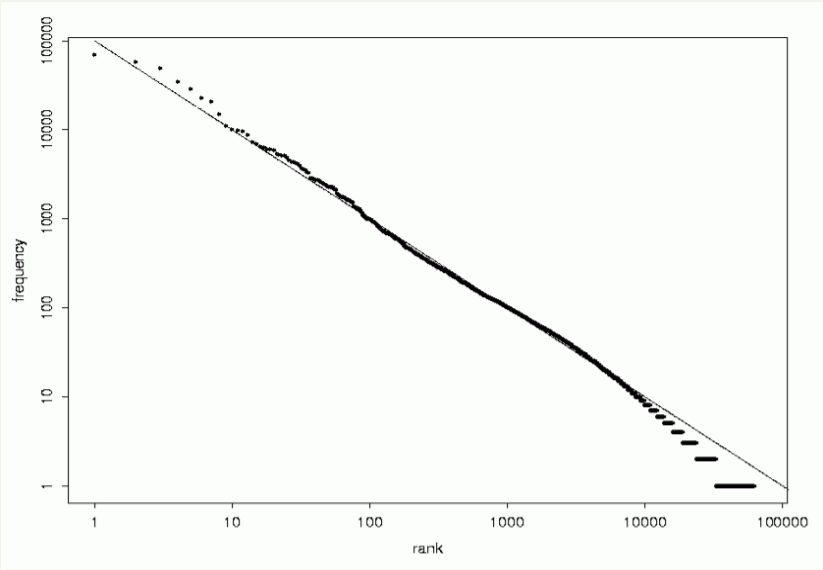
\includegraphics[width=0.75\linewidth]{images/loglogzipflaw.png}
    \caption{Plot of the Zipf Law in a log log form where the x is the rank of the word and the y is the frequency.}
    \label{fig:loglogzipflaw}
\end{figure}
For the most frequent terms we are over the line and for the least frequent terms we are below the line, but in the middle we are exactly on the line.\newline
In the following Figure \ref{fig:loglogzipfs} it has been shown how the plot looks with different slope.
\begin{figure}
    \centering
    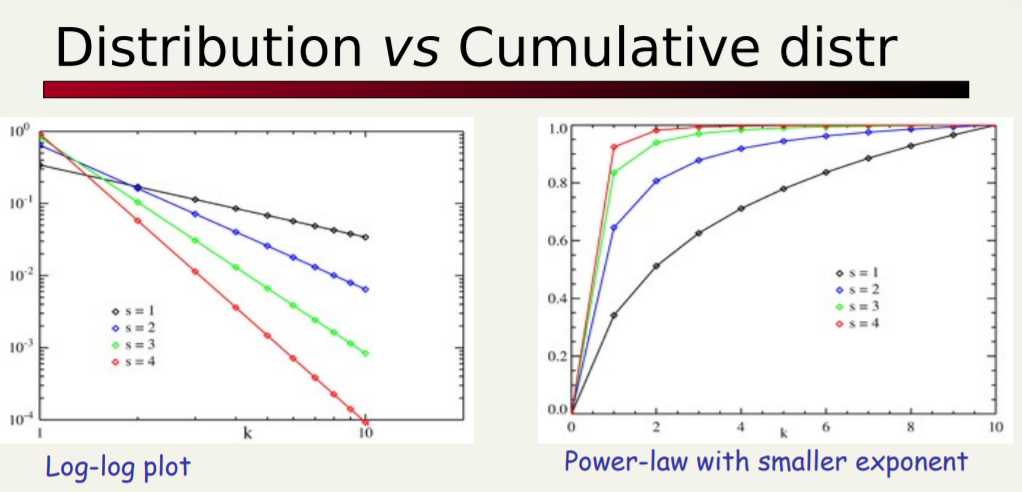
\includegraphics[width=0.75\linewidth]{images/loglogzipfs.png}
    \caption{On the left the log-log plot with different slope; on the right the cumulative distribution.}
    \label{fig:loglogzipfs}
\end{figure}
There is another important statistical property of the text that it's called \textbf{Heaps Law} for which the number of distinct tokens grows $n^\beta$ where $\beta<1$ typically 0.5 where n is the total number of tokens; the average token length grows as $\Omega(log n)$.\newline
Another property is the \textbf{Luhn Law} (empirical) for which interesting words are the ones with medium frequency and it can be seen in the following Figure \ref{fig:luhnlawplot} we can infer this from the fact that the most common words are the stop words that aren't so helpful and at the end we have very rare words that are not so important.
\begin{figure}
    \centering
    \includegraphics[width=0.75\linewidth]{images/luhnlaw.png}
    \caption{Plot Luhn Law.}
    \label{fig:luhnlawplot}
\end{figure}
\chapter{Index Compression}
In this chapter we are going to see which techniques are used to represent the dictionary because we want a data structure to store the tokens produced thanks to the operations described in the last chapter. In our case our tokens are string so we have a data structure to store strings and we want a compact data structure in order to save space (save some money) and in order to keep more stuff in memory (increasing speed). Notice that in general if we read compressed data and then we decompress them is faster than if we read uncompressed data because the decompression algorithms are very fast.\newline
Let's do some considerations about \textbf{Lossless Compression} vs. \textbf{Lossy Compression}:
\begin{itemize}
    \item \textbf{Lossless Compression:} all information is preserved; we maintain information;
    \item \textbf{Lossy Compression:} discard some information; we lose some information;
\end{itemize}
We will focus our topics on Lossless Compression instead examples of Lossy Compression are the previous operations because we throw away conjunctions.\newline
A first question that we can make ourselves is \textbf{how big is the term vocabulary?} this means how many distinct words are there? Can we assume an upper bound? not really even if some people think that reached a certain number of documents after that the dictionary will not increase anymore, but this is not true because the vocabulary will keep growing with the collection size especially with Unicode.\newline
There is a law that it's the \textbf{Heaps' Law:} $M=k*T^b$ where T is the total number of tokens in a collection and M is the number of the unique token (the size of vocabulary) and where $30 <= k <= 100$ and $b \approx 0.5$. So M is proportional to the square root of the total number of the tokens in the collection.\newline
Even in this case you can plot this with a log-log plot of vocabulary size M vs T and Heaps' Law predicts a line with slope about 1/2. In the following Figure \ref{fig:heapslaw} it has been shown the result of the log-log plot.
\begin{figure}
    \centering
    \includegraphics[width=0.75\linewidth]{images/heapslaw.png}
    \caption{Heaps'Law log-log plot where x is the total number of tokens in a collection and y is the number of the unique token.}
    \label{fig:heapslaw}
\end{figure}


Now we will consider compressing the space for the dictionary and postings because a search begins always with the dictionary and we want to keep it in memory; we have to consider even that embedded/mobile devices may have very little memory and even if the dictionary isn't in memory we want it to be small for a fast search startup time.\newline
The simplest data structure to store the dictionary is \textbf{array of fixed-width entries} basically I have a table with three columns and the first one is the column \textit{Term} where I allocate for all the rows a space that it's equal to 20 bytes; in the second column I have the \textit{frequency} for which I allocate 4 bytes; the last column is \textit{Postings pointer} that point to the postings list and it's 4 bytes too. We can see in the following Figure \ref{fig:arrayfixedwidth} the structure of this data structure.\newline
\begin{figure}
    \centering
    \includegraphics[width=0.75\linewidth]{images/arrayfixedwidth.png}
    \caption{Structure of Array of Fixed-width.}
    \label{fig:arrayfixedwidth}
\end{figure}
The first thing that we can highlight is that fixed-width term are wasteful because most of the bytes in the term column are wasted since we allocate 20 bytes for one letter terms and if we have very long words we still can't handle them. It has been seen that typically written English averages take 4.5 character/word, but I should not consider this average instead I should consider the average dictionary word in English that it's around 8 characters (there is this difference because in a dictionary we encounter each word once and instead in written English I en-count several times a word). Now the first question that we make is why don't we use this average? Because short words dominate token counts but not type average.\newline
A second data structure to compress the dictionary is \textbf{Dictionary-as-a-String} where I sort all the terms and then I store the dictionary as a (long) string of characters and a pointer to next word shows end of current word with this technique I can save up to 60 \% of dictionary space. I need only to store a table with three columns where the first column is the number of occurrences; the second column is the postings pointer; the last column is the term pointer. In the following figure Figure \ref{fig:dictionaryasastring} it has been shown the structure of this data structure.\newline
\begin{figure}
    \centering
    \includegraphics[width=0.75\linewidth]{images/dictionaryasastring.png}
    \caption{Structure of Dictionary-as-a-String.}
    \label{fig:dictionaryasastring}
\end{figure}
The space required for a dictionary as a string is:
\begin{itemize}
    \item 4 bytes per term for frequency;
    \item 4 bytes per term for pointer to Postings;
    \item 3 bytes per term pointer;
    \item average 8 bytes per term in term string;
\end{itemize}
Now the average is 11 bytes instead of 28 bytes. Supposing that I have 400k terms then the space required will be 400K*19 bytes that it's equal to 7.6MB against 11.2MB for fixed width.\newline
We can create a variant of this data structure where instead of using a term pointer for each word of the dictionary I use a term pointer each (for example) k=4 words of the dictionary such that we are saving 9 bytes on 3 pointers. This technique is called \textbf{Blocking} where we store pointers to every k-th term string, but in order to do this we need to store term lengths at the beginning of the term (it requires 1 extra byte). In general we can say that we lose 4 bytes for each block (to save the length), but we are saving 9 bytes on 3 pointers. In the following Figure \ref{fig:blocking} we can see the structure of Blocking with Dictionary-as-A-String.\newline
\begin{figure}
    \centering
    \includegraphics[width=0.75\linewidth]{images/blocking.png}
    \caption{Structure of Blocking with Dictionary-as-a-String.}
    \label{fig:blocking}
\end{figure}
A natural question that we do is at this point why don't we use a larger k in order to save more space? Yes if we increase k we save more space, but we will waste our time when we have to search a term because we go to the first term pointer, but then we need to scroll all the string until we reach the position of our term (we do a sequential scan).\newline
Now let's have a look at how search works. Let's analyze \textbf{Dictionary search without blocking} and this is the structure Fig.\ref{fig:dictionarysearchwithout}, notice that we \textbf{don't have a tree} like in the Figure it has been used to show how binary search works because when we do a search we just start from the element in the middle and then we proceed with a binary search. In this case what is the number of comparisons that we do? We can compute it from 1 comparison because we start from "job" then we do 2 times 2 comparisons because if "job" wasn't our goal we continue and we compare "den" or "pit" and so on. That's why at the end we get $(1+2*2+4*3+4)/8 \approx 2.6$.\newline
\begin{figure}
    \centering
    \includegraphics[width=0.75\linewidth]{images/dictionarysearchwithout.png}
    \caption{Dictionary Search without blocking.}
    \label{fig:dictionarysearchwithout}
\end{figure}


Now analyze the other case that it's \textbf{Dictionary search with blocking} where I am indexing only one word every k looking at the example we are indexing only "aid" and "job" the structure will be different; look at the Figure \ref{fig:dictionarysearchwith}. In this case we will start from "job" and then we will move to "aid" if our query is "smaller" than "job", but once we reach "aid" we need to scroll the list so I'm doing a sequential scan.\newline
\begin{figure}
    \centering
    \includegraphics[width=0.75\linewidth]{images/dictionarysearchwith.png}
    \caption{Dictionary Search with blocking.}
    \label{fig:dictionarysearchwith}
\end{figure}
In this case the number of comparisons in average is: (1+2*2+2*3+2*4+5)/8 = 3 comparisons and it's not so convenient like when we don't have blocking. So it's a trade-off between space to store the dictionary and the time to execute a query.\newline


The last technique that we are going to see in this chapter is the \textbf{Front Coding} for which sorted words commonly have long common prefix so the idea is to store only the differences. An example has been shown in the following Figure \ref{fig:frontcoding}. This technique is dependent on the size of the dictionary because if it's small it's not so probable that near terms share a lot of prefix instead if we have a large dictionary it's more probable.\newline
\begin{figure}
    \centering
    \includegraphics[width=0.75\linewidth]{images/frontcoding.png}
    \caption{Front Coding Technique}
    \label{fig:frontcoding}
\end{figure}
At the end we can do a small wrap up to see the performance of the techniques described above looking at this Figure \ref{fig:wrapupdictionary}.\newline
\begin{figure}
    \centering
    \includegraphics[width=0.75\linewidth]{images/wrapupdictionary.png}
    \caption{Table to summarize all the techniques.}
    \label{fig:wrapupdictionary}
\end{figure}
Until this moment we have seen that the searching operation is done by the binary search, but there are other options for searching the head words. In general there are three options:
\begin{itemize}
    \item \textbf{Binary Search};
    \item \textbf{Hash Table};
    \item \textbf{Trie};
\end{itemize}
In general the Hash Table is very good except when we have many collisions, but it can be built using perfect hashing that allows us to avoid collisions. Now maybe we are thinking "okay let's use hash table with perfect hashing and we avoid collisions" yes we can do this, but in general Hash Table doesn't support \textbf{Prefix Search} that's why in practice it's not used where prefix search means I want to find all the words that start with my query and not an exact search where I want the word that exactly match my query.\newline
The last solution that it's used because it supports prefix search is the \textbf{Trie} this is a data structure that has the shape of the tree and it has a character for each edge like in the following example Figure \ref{fig:trie}.\newline
\begin{figure}
    \centering
    \includegraphics[width=0.75\linewidth]{images/trie.png}
    \caption{Example of the data structure trie.}
    \label{fig:trie}
\end{figure}
I am representing words as paths and if the same prefix appears many times I need only to add the different characters at the end. This is efficient, but we have to be aware with cache misses also because we are using pointers so it's not a compact representation since pointers take a lot of space. There are many variants of this data structure and one of them is the so called \textbf{Compact Trie} in which every time I have nodes with out-degree equals to 1 I just compact it using one edge and now instead of having one character on that edge I have a sequence of characters, this is better because in this way we have reduced the number of nodes and the number of pointers. There are even \textbf{Pointerless representations of Tries} and these are even more compact, but they are less efficient in search operations.\newline
\chapter{Spelling Correction}
In the words that compose the query of the words of the documents we can find errors where some words contains wrong characters and to solve this problem we introduce the idea of \textbf{Spelling Correction}.
The spelling correction is not strictly required, but in practice is very useful and usually it's provided even in small systems.\newline
The spell correction has two principal uses:
\begin{itemize}
    \item Correcting documents being indexed;
    \item Correcting queries to retrieve "right" answers;
\end{itemize}
There are two kind of spell correction:
\begin{itemize}
    \item \textbf{Isolated Word:} check each word on its own for misspelling, but it's not the best choice because if I write "form" it's hard to understand if I meant "from" or the word is right;
    \item \textbf{Context-sensitive:} this case is more effective because we look at surrounding words for example if I write "I flew form Heathrow to Narita" it's clear that I meant "from";
\end{itemize}
The fundamental assumption is that we have a set of terms that we consider "correct" and they can be the terms in our dictionary or we can use a standard \textbf{lexicon} such as one provided by a dictionary or a lexicon specific to a particular application; in few words we have a set of words which are the correct ones and each time we find a term that it's not in our lexicon we try to correct it looking for the "closest" one.\newline
So basically the idea is given a lexicon and a character sequence Q we want to return the words in the lexicon closest to Q, but what does "closest" mean? There are several measures like:
\begin{itemize}
    \item \textbf{edit distance};
    \item \textbf{weighted edit distance} (that keeps track of the most common typing error);
    \item \textbf{n-gram overlap};
\end{itemize}
The first idea that come out is the \textbf{Brute-force approach} where given a query Q we enumerate all character sequence within a preset (weighted) edit distance for example 2 (two characters less or two characters more or two characters wrong) then we intersect this set with the list of "correct" words (lexicon) and you show terms you found to user as suggestions as the term suggests it's a brute force so it's not so efficient.\newline
What is the \textbf{edit distance}? Let's define it: given two strings $S_1$ and $S_2$ the edit distance is the minimum number of operations to convert one to the other. Operations are typically character-level we can do insert, delete, replace and possibly transposition.\newline
For example the edit distance from "dof" to "dog" is just 1; from "cat" to "act" is just 2 (1 with transposition); from "cat" to "dog" is 3.\newline
Generally the edit distance is found by dynamic programming and in the following Figure \ref{fig:pseudocodedit} we can see the pseudo-code. 
\begin{figure}
    \centering
    \includegraphics[width=0.75\linewidth]{images/pseudoedit.png}
    \caption{Pseudo-code of the edit distance.}
    \label{fig:pseudocodedit}
\end{figure}
We start initializing the first row and the first column starting from 0 and then increasing by 1 the error (notice that we need to add the \textbf{empty string}) then if we have a match at the i-th step we take the previous edit distance otherwise we take 1 + the minimum between the previous edit distance, the edit distance with one char less of the string one or the edit distance with one char less of the string two. In the following Figure \ref{fig:editdistancexample} it has been shown an example on how to compute the edit distance between two strings ("patt" vs. "pttapa").\newline
\begin{figure}
    \centering
    \includegraphics[width=0.75\linewidth]{images/exampleditdistance.png}
    \caption{Example of computing the edit distance with dynamic programming.}
    \label{fig:editdistancexample}
\end{figure}
Now let's focus on the \textbf{cost} where the computation of the exact edit distance takes O(|$S_1$|*|$S_2$|) time that it's \textbf{quadratic} and clearly it's not the best thing to do. More in general I'm not interested in computing the exact edit distance, but in computing the edit distance up to D (I accept up to D errors); there is an efficient algorithm to do this that takes linear time for a constant D: O(D*max(|$S_1$|,|$S_2$|)) in particular there are also very efficient bit-parallel algorithms.\newline


In Information Retrieval systems it makes sense to use a \textbf{Weighted Edit Distance} where the weight of an operation depends on the characters involved for example if the keyboard error is "m" when we wanted to write "n" it's considered a small error (it means small cost) instead if we wrote "q" then it's considered a big error (it means big cost) because it's more likely to be mis-typed as "m" than as "q". This approach requires a weighted matrix as input and needs to modify the Dynamic Programming to handle weights.\newline
\section{One-Error Correction}
The idea of checking the edit distance between my word and all the words in the dictionary is interesting, but it works only from a theoretical point of view. For this reason in this section we are going to consider an alternative way to correct our word where we admit only one error (this is simpler to do).\newline
With \textbf{1-error} we refer to insertion, deletion or substitution of one single character. For example if our query is:
\begin{itemize}
    \item Farragina -> Ferragina (substitution);
    \item Feragina -> Ferragina (insertion);
    \item Ferrragina -> Ferragina (deletion);
\end{itemize}
So if we have a string of length L over a characters it means that \textit{number of variants=L*(A-1)+(L+1)*A+L=A*(2L+1)} where L*(A-1) corresponds to a substitution, (L+1)*A corresponds to an insertion and L corresponds to a deletion.\newline
A possible approach that we can do \textit{assuming a fast string-check} in a dictionary is to create two dictionaries: D1={strings} and D2={strings of D1 with one deletion}. In the following Figure \ref{fig:exampletwodictionaries} it has been shown an example with two dictionaries.\newline
\begin{figure}
    \centering
    \includegraphics[width=0.75\linewidth]{images/exampletwodictionaries.png}
    \caption{Example with two dictionaries.}
    \label{fig:exampletwodictionaries}
\end{figure}
When we have to do a search we go to D1 for an exact search and then we go to D2 for one-error search.\newline
Now suppose that the query is "cat" we can have different cases:
\begin{itemize}
    \item \textbf{Perfect match}: when I do search(P) in D1, 1 query -> "cat";
    \item \textbf{P 1-char less}: when I do search(P) in D2, 1 query -> "cat" ["cast"];
    \item \textbf{P 1-char more}: when I do search(P -1 char) in D1, I do p queries so I search for {"at", "ca", "ct"} in D1 (in this example I don't have any match);
    \item \textbf{Substitution}: when I do search(P -1 char) in D2, I do p queries so I search for {"at", "ca", "ct"} in D2 (at[cat], ct[cat], ct[cst], ca[cat]);
\end{itemize}
So in general doing queries to the two dictionaries I can solve all the possible cases that I can have with one error.\newline
More in detail if we have:
\begin{itemize}
    \item \textbf{Perfect Match}: search for P in D1 (1 query) - in this case I know for sure the error=0;
    \item \textbf{P 1-char less}: search for P in D2 (1 query) - in this case I know for sure the error=1;
    \item \textbf{P 1-char more}: search for P-1 char in D1 (p queries) - in this case I know for sure the error=1;
    \item \textbf{Substitution}: search for P-1 char in D2 (p queries) - in this case I need to check the real error because it can be higher;
\end{itemize}
From this we can infer that we need 2p+2 hash computations for P.\newline
The \textbf{PRO} are that is CPU efficient, no cache misses for computing P's hashed; but O(p) cache misses to search in D1 and D2;\newline
The \textbf{CONS} are that we need large space because of the many strings of D2 which must be stored to search in the hash table of D2, unless we avoid collision (perfect hash);\newline
Consider that we can have \textbf{False Matches} (this is just a \textbf{filter}) because if we have "ctw" it will match "cat" and "cst" as a substitution (in D2 "ctw" becomes "ct" and "cat" with one char less is "ct") even if it's not a substitution.\newline
\subsection{Overlap Distance}
Before that we define what is the \textbf{overlap distance} we have to define what is the \textbf{K-gram index} that it's simply an index containing every k-gram (a substring of the term in the dictionary) for all the terms that appear in the dictionary.\newline
Notice that you \textbf{must} append (k-1) symbol \$ at the front of each string such that you can generate exactly L k-grams for a string of length L.\newline
In the following Figure \ref{fig:kgramindex} it has been shown an example of K-gram index where k=2.
\begin{figure}
    \centering
    \includegraphics[width=0.75\linewidth]{images/kgramindex.png}
    \caption{Example of K-gram index.}
    \label{fig:kgramindex}
\end{figure}
This approach is expensive because for each k-gram I mantain a list of all the possible terms associated to that k-gram.\newline
Now that we have defined what is the k-gram index we can explain the idea of \textbf{Overlap Distance}, given a query Q we enumerate all the k-grams in Q and to choose the "best" term we can see which term from the dictionary shares most k-grams with Q. So we use the k-gram index to rank all lexicon terms according to the number of matching k-grams with Q.\newline
In the following Figure \ref{fig:overlapdistancexample} we show an example of Overlap Distance for the query Q=mon=\{\$m, mo, on\}.
\begin{figure}
    \centering
    \includegraphics[width=0.75\linewidth]{images/overlapdistanceexample.png}
    \caption{Example of Overlap distance.}
    \label{fig:overlapdistancexample}
\end{figure}
One important thing that we can take into account is that a long word is more probable to share many k-grams with the other words (we can do something like the Jaccard similarity counting the number of intersections and the union of all the k-grams).\newline
The idea that we can apply is that we can use the overlap distance to \textbf{approximate} the edit distance. We can select terms by threshold on matching k-grams. So if the term is L characters long (it consists of L k-grams) and if E is the number of allowed errors (E*k of the k-grams of Q might be different from term's ones because of the E errors).\newline
This means that at least (L-E*k) of the k-grams in Q must match a dictionary term to be a candidate answer. If the edit distance is required then I can post-filter the results doing dynamic programming.\newline
Notice that this is a \textbf{necessary, but not sufficient condition} because it may happen that Q and T1 shares at least (L-E*k), but the edit distance is higher than E.\newline
An example can be "T=\$mom" and "Q=\$omo" then we have L-E*k=3-1*2=1 and we notice that T and Q share 2 elements so 2 >= 1 it means that they can have edit distance equals to E=1, but in reality the edit distance is 2. This approach gives us candidates, but not a correct value for this reason we use dynamic programming on candidate strings.\newline
Here Figure \ref{fig:exampletrigrams} we have an example with trigrams (k=3) and it has been shown what happens if the allowed error is 1 or 2. In any case we need post-filter to check the real edit distance in fact in this case the edit distance is higher than 2.\newline
\begin{figure}
    \centering
    \includegraphics[width=0.75\linewidth]{images/exampletrigrams.png}
    \caption{Example with trigrams (k=3).}
    \label{fig:exampletrigrams}
\end{figure}
Now to do a search we start from the bigrams of our query and then for each of them we compute the cardinality of the terms. Notice that each k-gram has a list of terms that are ordered in a lexicographical way so I need to compute the intersection between these lists (lists of the k-grams involved) and since they are ordered in lexicographical way the intersection is done by the \textbf{merge} (that we have seen with postings lists).\newline
\textbf{Observations}: we append \$ at the beginning of each string such that the number of k-grams for a string is exactly L. Now understand why we use the formula $L-e*k$ suppose that we have two strings s and Q and suppose that the i-th character is different. From this we know that due to the i-th character we have "killed" k k-grams because the i-th character appeared in the k-gram where the first item is the character i-th and so on until the i-th character is the last element of the k-gram. So \textbf{for each error we lose e*k k-grams} from this we have just said that the total number of k-grams is L so the shared k-grams are L-e*k. Unfortunately this formula is rough because as we said if there is an error I don't match the corresponding k-grams between s and Q, but it may happen that for example the third k-gram of s doesn't match with the third k-gram of Q, but with the twelfth k-gram of Q (for this we call them "candidate strings").\newline 


Now let's move to another topic always related to spell correction that it's \textbf{Context-sensitive} spell correction. We can understand this concept better with an example that we have already shown; suppose that the text is "I flew from Heathrow to Narita." and consider the phrase query "flew form Heathrow", we would like to respond: Did you mean "flew from Heathrow?" because none document matched the query phrase. This is done mainly using \textbf{heuristics}. \newline
We enumerate multiple alternatives and then we need to figure out which to present to the user for "Did you mean?" and as just said we use heuristics for example:
\begin{itemize}
    \item The alternative hitting most documents (look the most clicked documents similar to my query);
    \item Query log analysis (all the queries done in the system in the last few days) + tweaking for especially popular, topical queries;
\end{itemize}
Unfortunately the spell-correction is computationally \textbf{expensive} that's why it's run on queries that matched few documents.\newline


\section{Wild-card queries}
Until this moment we have seen simply queries, but let's have a look at some sophisticated queries let's analyze the so called \textbf{Wild-card queries}.
For example with:
\begin{enumerate}
    \item \textbf{mon*:} I'm looking for all the documents containing words beginning with "mon"; we use a \textbf{Prefix-search} data structure (to do this kind of queries we can't use hash tables);
    \item \textbf{*mon:} I'm looking for all the documents containing words ending with "mon"; we still use a prefix-search data structure for reverse terms (we will see how to do this soon);
    \item we can solve even queries like \textbf{pro*cent} and below we will see how to do that;
\end{enumerate}
The symbol * is called \textit{wild character}.\newline
To solve the third kind of query (where we have the wild character): suppose that our query is "co*tion" we could look up "co*" AND "*tion" and intersect the two lists, it's clear that this can work, but it's too expensive. Another problem can be the fact that if our query is "se*ate AND fil*er" this create many Boolean ANDs.\newline
The solution that it's used is to transform wild-card queries such that the "*"'s occur at the end; this solution gives rise to the \textbf{Permuterm index}.
Let's analyze the idea of \textbf{Permuterm Index:} for a term like "hello" we build an index under "hello\$", "ello\$h", "llo\$he", "lo\$hel", "o\$hell", "\$hello" where "\$" is a special symbol (notice that now in my dictionary I have added six different words, if l is the length of the word without the \$ then I will have L+1 words).
The query becomes:
\begin{itemize}
    \item X lookup X\$;
    \item X* lookup \$X*;
    \item *X lookup X\$*;
    \item *X* lookup X* (without "\$"!!);
    \item X*Y lookup Y\$X*;
\end{itemize}
The main query where we are more interested in is "P*Q" that as we said become "Q\$P". It has been shown an empirical \textbf{observation for English language} that the Permuterm problem requires $\approx 4x$ the lexicon size.\newline
\section{Soundex}
This is the last topic of this chapter and it's a technique which is designed to find words that are very different from the words that are typed. 
The \textbf{Soundex} is a class of heuristics to expand a query into phonetic equivalents and it's language specific and it's mainly used for names. For example if we write "Chebyshev", but we meant "Tchebycheff" (it's the name of a Mathematician). This technique has been invented for the U.S. census in 1918.\newline
The typical algorithm turns every token to be indexed into a reduced form consisting of 4 characters and when I receive a query I do the same so I turn every token in a reduced form. When I need to do a query I just search an index on the reduced forms.\newline
The main steps of the algorithm are:
\begin{enumerate}
    \item Retain the first letter of the word;
    \item Change all occurrences of the following letters to "0" (zero): "A", "E", "I", "O", "U", "H", "W", "Y";
    \item Change letters to digits as follows:
    \begin{itemize}
        \item B, F, P, V -> 1;
        \item C, G, J, K, Q, S, X, Z -> 2;
        \item D, T -> 3;
        \item L -> 4;
        \item M, N -> 5;
        \item R -> 6;
    \end{itemize}
    \item Remove all pairs of consecutive equal digits;
    \item Remove all zeros from the resulting string (are vowels [vocali] and letters that don't make any "noise");
    \item Pad the resulting string with trailing zeros and return the first four positions, which will be of the form <uppercase letter> <digit> <digit> <digit> (if the string is smaller then 4 char then I add zeros such that the length reaches 4);
\end{enumerate}
The Soundex is the classical algorithm, provided by most databases like Oracle, Microsoft and so on, but it's not very useful for information retrieval. It's okay for "high recall tasks" (like Interpol) though biased to names of certain nationalities, instead other algorithms for phonetic matching perform much better in the context of Information Retrieval.
\chapter{Keyword Extraction}
In this chapter we are going to exploit the statistical extraction. First of all we should define what is the \textbf{Collocation}? We talk about this when two or more words correspond to some conventional way of saying.\newline
The collocation has some features like:
\begin{itemize}
    \item \textbf{Limited compositionality:} meaning can't be fully inferred by its constitutent words for example "white wine" or "white hair";
    \item \textbf{Non substituability:} can't substitute other words and keep same meaning for example "yellow wine";
    \item \textbf{Non modifiability:} can't add lexical material otherwise an idiom would be changes;
\end{itemize}
The first approach that we can think to \textbf{extract collocation} to compute the collocation between two words is to consider all the possible pairs of words and count the frequency of them and then I sort by the frequency such that I know which two words appear most of the time together. We can see an example in the following Figure \ref{fig:collocationfrequencyex} and it's already clear looking the image what is the problem; since we already said that the most frequent words are the \textbf{stop words} (articles, adverbs and so on) I will not have significant information. We used this approach because we taught that more a collocation appear more is significant, but as we already said this is not always true.\newline
\begin{figure}
    \centering
    \includegraphics[width=0.75\linewidth]{images/collocationfrequencyex.png}
    \caption{Example of collocation by frequency.}
    \label{fig:collocationfrequencyex}
\end{figure}
\section{Tag Pattern}
A very effective idea that it's considered efficient is using the so called \textbf{Tag Pattern}. To exploit this we must introduce the \textbf{PoS tagging} that it's a parser and given a part of text we analyze the text and for each token we assign it a tag that it's a "letter" such that we can understand the "role" of the word inside the text. To be more clear we can understand it with an example, let's have a look at the Figure \ref{fig:tagpatternexample} where "A" stands for "adjective" and "N" stands for "noun" and "P" stands for "preposition". Notice that they can be formed by two or three words.\newline
\begin{figure}
    \centering
    \includegraphics[width=0.75\linewidth]{images/tagpatternexample.png}
    \caption{Tag Pattern example.}
    \label{fig:tagpatternexample}
\end{figure}
Given this tagging our goal is to apply the idea shown before that couldn't work - \textbf{frequency method} - with \textbf{PoS tagging} such that when we sort we consider only some \textbf{specific tag pattern}.\newline
We can see the results here Figure \ref{fig:frequencypostagging} where now the results are different because we filtered the frequency removing for example the tag pattern "AA" because it's useless. We can consider this as a good approximation, notice that we can still have some "useless information" like "last week" or "last year".\newline
\begin{figure}
    \centering
    \includegraphics[width=0.75\linewidth]{images/tagexample.png}
    \caption{Example of applying frequency + PoS tagging.}
    \label{fig:frequencypostagging}
\end{figure}
This is the most easy and effective way to extract collocations, but there is another approach that it's based on more sophisticated evaluation because it comes from the observation that sometimes it can happen that two words are not contiguous each other, we need \textit{flexibility}. Look at this Figure \ref{fig:flexibilityapproach} as you can see the words "knocked" and "door" aren't contiguous, but they often appear together.\newline
\begin{figure}
    \centering
    \includegraphics[width=0.75\linewidth]{images/flexibilityapproach.png}
    \caption{Example of words not adjacent to each other.}
    \label{fig:flexibilityapproach}
\end{figure}
The previous approach would lose this kind of collocations because they are not contiguous; the idea to find this kind of collocations is to have more flexibility so we need to evaluate the \textbf{mean} and the \textbf{variance}. So for each pair of words we compute the mean distance and the variance of the distance, but of course we need a \textbf{window} to do that because we can't consider all the possible pairs otherwise it will be too expensive to compute.\newline
In the following Figure \ref{fig:distancedistribution} (in the first plot) we can see an example of distance distribution where on the y we have the frequency of "strong" and on the x we have the position of "strong" w.r.t. "support" for example usually "strong" appears before of "support", but sometimes it happens that it appears after. You can see from the plot that the mean distance is small and variance too, instead in the second plot where we compare "strong" and "for" the mean is small, but the variance is high and we call this \textbf{bi-modal distribution} from this we infer that it's not an interesting pair.
\begin{figure}
    \centering
    \includegraphics[width=0.75\linewidth]{images/exampledistancedistribution.png}
    \caption{Example of Distance Distribution.}
    \label{fig:distancedistribution}
\end{figure}
Here we have another example Figure \ref{fig:distancedistribution2} from which we deduce that an high s means that it's not an interesting relation, but if d>0 (small in general) and s is very small then we have an interesting phrase. Notice that this is not necessarily true because it's just a statistical test.\newline
\begin{figure}
    \centering
    \includegraphics[width=0.75\linewidth]{images/exampledistance2.png}
    \caption{Another example of distance distribution.}
    \label{fig:distancedistribution2}
\end{figure}
We can improve this approach using a \textbf{query log} (queries that have been done by the users) because we can consider this text to find new collocations and to find interesting pairs. For example if we look at the previous example we can see that "Garrison" and "said" is selected, but to be sure that it's a collocation we can look at the query log and if in millions of queries these two words don't appear together then we discard them otherwise it means that they are an interesting pair of words.\newline
\section{Pearson's chi-square test}
A third test which is very effective from a statistical point of view is the \textbf{Pearson's chi-square test} that we are going to analyze it only for \textit{bigrams}.\newline
Let's look at the idea behind this test: we compare the frequency of occurrences of a pair in a data-set (taking a collection of documents) against a statistically uniform distributed text and if the pair has a frequency which is in some sense close by the frequency of the two individual words just taken in a random way then this is not a significant pair because it's almost similar to a normally distributed data. Instead if it's different we can consider the two words as a collocation, but to understand this better let's have a look at the image Figure \ref{fig:pearsonchisquare} where on the x axis we have the so called \textbf{Pearson's cumulative test statistic}. The Pearson's cumulative test gives us a value and larger is this value it means that more the two words are not randomly distributed so the larger is the value (depending on some parameter that we call \textit{k} and it's the \textbf{degree of freedom}) smaller is the probability that the two words come from a random data-set. On the other hand on the y axis we have significance in statistical terms of this test so if we want that our confidence about the fact that they are not randomly distributed is very high then we can get the chi-square that allows us to get this confidence on the conclusion.\newline 
\begin{figure}
    \centering
    \includegraphics[width=0.75\linewidth]{images/pearsonchisquare.png}
    \caption{Plot of the Pearson's Chi-Square Test.}
    \label{fig:pearsonchisquare}
\end{figure}
Let's look at this Figure \ref{fig:examplechisquare} where we have an example of Chi-Square Test and assume that we test if the words "new" and "companies" are a good pair so we create a matrix 2x2 and in every cell we write the frequency (to understand it better look at the image). Now see what is the \textbf{degree of freedom} if we have a table with \textit{r} rows and \textit{c} columns there are \textbf{(r-1)*(c-1) degrees of freedom}. So now that we have understood this in the previous Figure \ref{fig:pearsonchisquare} we must consider k=1 because at the start of this section we said that we consider only bigrams.\newline
\begin{figure}
    \centering
    \includegraphics[width=0.75\linewidth]{images/examplechisquare.png}
    \caption{Example of Chi-Square test.}
    \label{fig:examplechisquare}
\end{figure}
Now continue following this example and let's establish the significance of a collocation that it's the Chi-Square Test and it's computed according to:
\begin{equation}
    X^2=\sum_{i,j}\frac{(O_{i,j}-E_{i,j})^2}{E_{i,j}}
\end{equation}
where O is the \textbf{observed frequencies} (in other words it's in our table) and E is the \textbf{average frequency} if the words would be taken independently at random that it's equal to $E_{i,j}=N*freq(i)*freq(j)$.\newline
What we get from $X^2$ is (I haven't reported all the steps to reach it):
\begin{equation}
    X^2=\frac{N*(O_{11}O_{22}-O_{12}O_{21})^2}{(O_{11}+O_{12})(O_{11}+O_{21})(O_{12}+O_{22})(O_{21}+O_{22})}=1.55
\end{equation}
Now that we get this new value our question is: \textbf{Is 1.55 a good value to consider these two words as a "good" collocation?} to do this we need to consider the following table Figure \ref{fig:tablefreedom} and we must consider the first row because d.f. stands for "degree of freedom" so since we said that our d.f. is one we consider that row. Then we consider a P-value=0.10 (significance of our precision and in this case is 90\% because we chose it 0.10 that it's the error) and looking at that entry we have as result 2.71. Now we have to compare the reference value (2.71) with the value that we got from the formula (1.55) since 1.55<2.71 then we infer that the two words are not a significant collocation otherwise if the value that we obtained from the formula was bigger of 2.71 it meant that the two words weren't close each other randomly. When happens that the two words aren't considered a good pair we say that \textbf{the null hypothesis is plausible} and for this reason from a statistical point of view the words aren't selected.\newline
\begin{figure}
    \centering
    \includegraphics[width=0.75\linewidth]{images/tablefreedom.png}
    \caption{Table Degree of Freedom.}
    \label{fig:tablefreedom}
\end{figure}
\section{RAKE Rapid Automatic Keyword Extraction}
Now let's introduce a software which is very simple and heuristic so it hasn't statistical guarantees, but it's interesting because it doesn't need a lot of data.\newline
RAKE is based on the following properties:
\begin{itemize}
    \item Works on single/few (not much long) documents so it doesn't need a large data collection;
    \item Easily applicable to new domains because you don't need a "training set";
    \item Fast;
    \item Unsupervised (it's not totally correct to use this term because we need to set some parameters to use the software in a good way);
\end{itemize}
The \textbf{key observation} of this approach is that \textit{keywords frequently contain multiple words but rarely contain punctuation or stop words} (this is an obvious observation) and is the key above the RAKE software is built upon.\newline
The RAKE pipeline consists in a set of steps. First of all we have to define the input parameters (or we can use the default ones):
\begin{itemize}
    \item a set of word delimiters (like "," or " ");
    \item a set of phrase delimiters (like "." or one entire blank line);
    \item a list of stop words or stop-list (like the articles or the propositions);
\end{itemize}
\textbf{Step 1: Candidate Keywords}
\begin{itemize}
    \item The document is split into an array of words by the specifies word delimiters;
    \item This array is split into sequences of contiguous words at phrase delimiters and then stop word;
    \item Words within a sequence are considered a candidate keyword;
\end{itemize}
In the following Figure \ref{fig:rakestep1} there is an example of this first step. At the first step we have a set of candidate keywords and this process is very fast and simple.\newline
\begin{figure}
    \centering
    \includegraphics[width=\linewidth]{images/examplestep1.png}
    \caption{Example of Step 1 on RAKE.}
    \label{fig:rakestep1}
\end{figure}
\textbf{Step 2: Scoring Candidate Keywords} (we score the candidate keywords and then we will sort them according to the score)
\begin{itemize}
    \item Compute the table of co-occurrences (we do filtering in the sense that we want to throw away keys that are not interesting); In this phase we create a table where the rows and the columns are the words so it will be a matrix $nxn$ where n is the number of terms that we are analyzing;
    \item And few metrics like \textit{freq(w)}= total frequency on diagonal (if you look at the Figure of the second step we see that on the diagonal we write the occurrences of that words for example "algorithms" occurs 2 times in the result of the first step and "bounds" 1 time) or \textit{deg(w)}= sum over row (is the sum of the elements in that row for example for the word "algorithm" the degree is 3 and for "bounds" the degree is 2);
\end{itemize}
In the following Figure \ref{fig:rakestep2} we can see an example of the second step where we will use some statistics tools. Our goal in this step is to score the keywords and then sort them. From the table we can understand several things because for example if the degree and the frequency of a word are highly different then it means that algorithms occurs many times alone and few times with other words so it's probably better an individual word. Then what we compute is the \textbf{ratio} (deg(w)/freq(w)) because degree and frequency give us an idea on how some words are good with others or not and the ratio is our \textit{scoring mechanism}. To compute the \textbf{score of the keywords} is the sum of the scores of every individual words.\newline
\begin{figure}
    \centering
    \includegraphics[width=\linewidth]{images/examplestep2.png}
    \caption{Example of Step 2 on RAKE.}
    \label{fig:rakestep2}
\end{figure}
From this we compute the score of keywords found at the first step just summing the individual score like in the Figure \ref{fig:step2scoring} where we have sorted by decreasing score (obviously it happens that the score is higher for keywords with many words).\newline
\begin{figure}
    \centering
    \includegraphics[width=\linewidth]{images/step2scoring.png}
    \caption{Example of Step 2 on RAKE with keywords score.}
    \label{fig:step2scoring}
\end{figure}
In the following Figure \ref{fig:resultrake} we can see the comparison between the result of RAKE tool against the result of a Manually assignment by humans and there are three false positives (keywords chosen by the software, but not by the humans) and one false negative (keyword chosen by the humans, but discarded by the software); in any case the results are pretty similar. The differences comes from the fact that RAKE doesn't do any post-processing operations because for example "set of natural numbers" is not taken by the software due to the presence of "of". In order to avoid this limitation RAKE does the step 3.\newline
\begin{figure}
    \centering
    \includegraphics[width=\linewidth]{images/resultrake.png}
    \caption{Result RAKE vs. Manually Assigned.}
    \label{fig:resultrake}
\end{figure}
\textbf{Step 3: Adjoining keywords}\newline
In this step we identify keywords that contain interior stop words such as "axis of evil". So what we do is:
\begin{itemize}
    \item Looks for pairs of keywords that adjoin one another \textbf{at least twice} in the same document and in the same order;
    \item The score for the new keyword is the \textbf{sum} of its member keyword scores ("of" doesn't have any score we consider only "axis" and "evil" scores);
\end{itemize}
\textbf{Step 4: Selecting keywords}\newline
In this case we usually choose the top one-third keywords. For example if we have 30 keywords we choose the first 10.\newline
If we look back at the result of Figure \ref{fig:resultrake} we had the false negative "set of natural numbers" because that keywords appeared just once if they appeared two times the RAKE would chosen them thanks to step 3 of the tool.\newline
\chapter{Query Processing}
In this chapter we are going to discuss about the query processing. First of all we start from \textbf{Phrase queries} where we want to be able to answer queries such as "Stanford University" as a phrase thus the sentence "I went at Stanford my university" is not a match because we want \textbf{exactly} "Stanford University" (we want that the two words are contiguous).\newline
\textbf{Solution 1 - 2-word indexes:} the first solution that came out in our mind is to use collocations; for example if our text is "Friends, Romans, Countrymen" we would generate the bi-words  "friends Romans" and "Romans countrymen" and each of these 2-words is now an entry in the dictionary.\newline
Usually if people search for longer phrases queries we process them by reducing them to bi-words queries in AND. For example "Stanford university Palo Alto" can be broken into the Boolean query on bi-words such as "stanford university" AND "university palo" AND "palo alto"; in this way I can find each pair in the \textbf{2-word index} finding the postings list and then I merge them. Notice that I can't always find the right solutions, but I can have false positives because the index blows up we only find a \textbf{superset of answers}; let's understand this better for example if we have that the pair "stanford university" appears in the document 3 and even the pair "palo alto" appear there it doesn't mean that they are contiguous because we don't know. If we want to be precise we should check the documents to be sure that the pairs are contiguous and this process can be very slow.\newline
\textbf{Solution 2 - Positional indexes:} to solve this problem we make a small change to the postings because we store for each term and document the position(s) in which that term occurs. The scheme will be something like this: <term, number of docs containing term; doc1: position1, position2,...; doc2: position1, position2,...; etc>. In this solution we apply the merge algorithm "two times" because we apply it to find shared documents, but even shared position that it's shifted by one because obviously different words can't stay in the same position in the same document.\newline
In the following Figure \ref{fig:phrasequerypositionalindexes} we have an example of a Phrase Query solved with positional indexes.\newline
\begin{figure}
    \centering
    \includegraphics[width=0.75\linewidth]{images/phrasequery.png}
    \caption{Example of Phrase Query with positional indexes.}
    \label{fig:phrasequerypositionalindexes}
\end{figure}
This approach is very very powerful because it's not used only be the search engines to solve phrase queries, but is done even to solve \textbf{proximity queries}. It can be used even to give a score to the pages because for example pages with close words are more relevant than pages with far words for example if we have a page with "Paolo" and "Ferragina" close each other then it's considered a good page, but if we have that the first word is "Paolo" and the last word of the document is "Ferragina" then it means that it's not considered a good page.\newline
To solve \textbf{proximity queries} we don't care about the order because we don't have the quotes ("") so in general when we match the documents then we move to checking the words positions and we compute the minimum distance between the positions and we move on the minimum; to understand this better if we look at the previous example when we match the document 4 we compare 8 with 17 and we compute the distance that it's 9 then we move on the minimum and we compare 16 with 17 and now the distance is 1 so we have found a smaller distance (notice that we compute the absolute value because we don't care about the order of the words).\newline
At the end we can say that \textbf{Positional indexes} are good to compute \textbf{Phrase Queries} and \textbf{Proximity Queries} too.\newline
Now let's make some considerations about the positional index size; it's clear that the size now is much bigger because we are storing the positions too for each document, but anyway we can use compression and some tricks since the positions are integers. It has been shown that the positional index expands postings storage by a factor 2-4 for English words so if before the index required 100Mb now it will require 400Mb.\newline
\textbf{Combination schemes:} we can combine 2-Word with Positional index because 2-word is particularly useful for particular phrases like "Michael Jackson" or "Britney Spears", but it's clearly that it's more complicated to solve.\newline
\textbf{Soft-AND:} it was used at first by Google, but nowadays it's used by most of the search engines. The Soft-AND idea is that the AND is too strong and then we can possibly miss some documents that are interesting; let's see how it works through an example.\newline
Suppose that the query is "rising interest rates":
\begin{itemize}
    \item Run the query as a phrase query;
    \item If <K documents contain the phrase "rising interest rates", run the two phrase queries "rising interest" and "interest rates" (we are "relaxing" the query);
    \item If we still have <K documents, run the "vector space query" "rising" "interests" and "rates";
    \item "Rank" the matching documents;
\end{itemize}
We see this technique when we make a query on Google and they "cancel" some terms when our query is very strict.\newline
\section{Caching for Faster Query}
Let's go to another issue to address in query processing that it's the caching in order to speed up the query.\newline
There are two opposite approaches that can be used in combination:
\begin{itemize}
    \item Cache the query results (exploits query locality); for example if many people are searching for "Mario Draghi" we save in the cache these results because it's useless each time to process the entire query; if we look at the Figure \ref{fig:queryresults} this approach is the one in the box "Result Cache"; this approach has some weakness like \textbf{cache consistency} because for example since we save it in the cache then it means that it's very search by the people and probably it's related to some news that means we don't have always the "fresh news" (the results change every minute);
    \item Cache pages of posting lists (exploits term locality); for example if many people search for "Mario Draghi Finanziaria" or "Mario Draghi Legge Finanza" instead of saving the results we save the posting lists; if we look at the Figure \ref{fig:queryresults} it's called "List Cache"; if someone searches for "Mario Draghi Europa" then we have already "Mario Draghi" list; even in this case we can have \textbf{cache consistency};
\end{itemize}
\begin{figure}
    \centering
    \includegraphics[width=0.75\linewidth]{images/queryresults.png}
    \caption{Structure on Query Caching.}
    \label{fig:queryresults}
\end{figure}
\section{Tiered indexes for faster query}
In this section we are going to describe another technique to speed up the computation of the queries that it's called \textbf{Tiered indexes}.\newline
The idea behind this approach is to break posting lists up into a hierarchy of lists (first the most important and at the end the least important). What we get is: inverted index thus broken up into \textbf{tiers} of decreasing importance; it's good because we store the more important lists in the fastest memory and the less important lists in the secondary memory.\newline
When we make a query we use the top tier unless it fails to yield K documents if this happens then we drop to lower tiers.\newline
Here in the following Figure \ref{fig:exampletier} we can see an example of tiered index where the first tier stands for the most important lists and then the third tier is the less important lists. For example the posting list of the term "auto" is formed by document1 and document2 and since we inserted in the tier only the document2 it means that it's considered very important and instead the document1 is considered less important. Thanks to this approach we are able to find important documents in few time and for example if our query is "auto" AND "insurance" we are lucky because doing the intersection we find the shared document that it's document2, but on the other hand if we are looking for "auto" AND "car" when we do the intersection in the tier 1 we don't find any shared document so we need to go the other tiers. Notice that each list is sorted in its tier so for example the list of "car" in the tiers it's sorted only for their tier and for this reason we need to merge all the corresponding lists to do a merge.\newline
\begin{figure}
    \centering
    \includegraphics[width=0.75\linewidth]{images/exampletier.png}
    \caption{Example of tiered index.}
    \label{fig:exampletier}
\end{figure}
\section{Query Optimization}
Let's refresh a concept that we already discussed in the introduction chapter and it's the concept of \textbf{Skip Pointers} (at indexing time). Let's have a look at an example to understand it better (Figure \ref{fig:skippointers}) in the example we have partitioned the list into blocks of length 3 for the first list and into blocks of length 4 for the second list. Notice that the partition in the blocks it's up to us because it can be homogeneous or variegate and so on.\newline
\begin{figure}
    \centering
    \includegraphics[width=0.75\linewidth]{images/skippointers.png}
    \caption{Example of Skip Pointers.}
    \label{fig:skippointers}
\end{figure}
Obviously more skip pointers I use \textbf{more space} I need, but I increase the probability to jump a block (even if they are very small); on the other hand if I use less skip pointers then I use \textbf{less space}, but the probability to jump is smaller and if I jump I can jump a lot.\newline
\textbf{Trade-off:}
\begin{itemize}
    \item More skips -> shorter spans -> more likely to skip;
    \item Less skips -> longer spans -> few successful skips and less pointer comparisons ;
\end{itemize}
\textbf{How do we choose the block length?} In the worst case we use as block size $\sqrt{L}$ where \textit{L} is the length of the list such that the size of a block is equal to the number of the skip pointers. On the other hand if we know the probability distribution then things may change because for example if we know the score of some documents so we know that some documents are more required then other then we will use shorter block size when we know that in that section the score is high and longer block size when we know that in that section the score is low (documents are required rarely). In other words if a document is very high required it's not good to consider it in a long block size. To improve this approach we can use dynamic programming.\newline
This is definitely useful for in-memory index, but from an I/O point of view the cost of loading a bigger list can out-weight the gains.
\chapter{Compression of documents}
In this chapter we will see how compressed documents are stored in a search engine. The goal is that given a peer to peer system we want to keep aligned the documents exchanging between two nodes the minimum number of bits.\newline
The compression of documents is important because for example when we make a search on Google we see the so called \textbf{snippet} (few lines that show us the main content of a page) sometimes it's also called KWIC that stands for Keyword In Context.\newline
One of the most famous and old compressor is \textbf{gzip}, but during the years have been developed other compressors. For example Google developed \textbf{snappy} that it's a compressor different from the others that were born in that time because before people thought to create compressor that were able to squeeze a lot the size of the document, but the goal of Google was to create a "good" compressor in the sense to have even a fast decompression time. For example for Google was important that when someone does a query has fast results that means even fast snippet and to do that they need a low decompression time.\newline
In 2015 Google improved his compressor creating a new one called \textbf{Brotli}; after one year Apple created their own compressor that it's \textbf{LZFSE}; at the end there is even Facebook with \textbf{ZSTD} compressor.\newline
\section{LZ77 Compression}
All the algorithms that we have just described are based on the Lempel and Ziv's paradigm known as \textbf{LZ77} and it has been created in 1977; this algorithm is particular because it's a syntactic compressor, but achieves a good entropy (remember that with this word we mean that higher entropy corresponds to more information lost).\newline
\begin{figure}
    \centering
    \includegraphics[width=0.75\linewidth]{images/lz77.PNG}
    \caption{Example of LZ77.}
    \label{fig:lz77}
\end{figure}
\begin{figure}
    \centering
    \includegraphics[width=0.75\linewidth]{images/lz77window.PNG}
    \caption{LZ77 with window.}
    \label{fig:lz77window}
\end{figure}
With LZ77 we want to find the longest sub-string that matches with the previous characters; to understand how it works we are referring to the following Figure \ref{fig:lz77} where we compress the characters creating tuple formed by three items in this way: \textbf{<distance, length, next-char>} (sometimes they are called codeword or even phrases) and at each step we advance by length+1. We have to say that we use a \textbf{window} that has fixed length and moves at each step; we can see an example with window in the following Figure \ref{fig:lz77window}.\newline
A first question that we can do is: \textbf{Why do we need another character?} The answer is that we need it because it may happen we can't copy anything from the previous characters; the simplest example is when we start compressing and the previous characters are 0.\newline
During the years have been proposed many variations trying to improve some aspects like how to find the longest sub-string in an efficient way or using less objects instead of three.\newline
Notice that as we can see from the previous example the copy from the previous characters can \textbf{overlap} on the current string; we have overlapping when the field \textit{length} is larger than \textit{distance}.\newline
If we want to be honest we have to say that LZ77 it's not a real compressor, but it's a transformer because it transforms text into sequences of tuples composed by three elements and then you need other compressors to compress the tuples.\newline
If during our life we have used \textit{gzip} we have seen that there is an optional value we can choose between -1 and -9 and larger is this value then slower is the compressor because this value tells us how large is the window and -1 stands for 100 Kilobytes and -9 stands for 900 Kilobytes; in decompression is faster -9 because it possibly creates less phrases (we can possibly do "big jump") while -1 is slower because it possibly creates more phrases and we need to decompress we have to apply decompression at different positions.\newline
Let's see another example of overlapping and suppose that until this moment we have decompressed "abcd" and the next phrase/codeword that we see is <2,9,e> from this we can understand that now the string becomes "abcdcdcdcdcdce" and from this example we can see that it's so good when we have loop.\newline
From a technical point of view if we want to code this algorithm we can use the library \textbf{zlib} that it's no longer covered by patent so it's free even from a commercial point of view; if we continue talking about this library we have to say that when we use this function we have to pass the array corresponding to output and the first question that we do to ourselves is "how can I know what is the size?" for this reason we usually pass an array whose size is larger by 10/15\% of the original array because sometimes it can happen that the output (the set of codewords require more space of the original text), but then we can reduce the size of the array if we receive in output codewords that require less space.\newline


Now we have to introduce another website that it's \href{https://quixdb.github.io/squash-benchmark/}{Squash Compression Benchmark} a compression benchmark from which you can choose the collection of files where you want to do your tests and you can choose the machine to do the benchmark on; notice that changing the machine the performance are different.\newline
Look at the following Figure \ref{fig:plotratio} this is a typical plot because usually if we have a good compression ratio (y axis) then the decompression speed is low (x axis) for this reason it's like a trade-off between high compression ratio and high decompression speed. Be careful that we must not care only about the compression because in several applications we have even the transfer time (networking systems) that it's added to the decompression time.\newline
\begin{figure}
    \centering
    \includegraphics[width=0.75\linewidth]{images/compressionratio.PNG}
    \caption{Plot where on x we have decompression speed and on the y we have compression ratio.}
    \label{fig:plotratio}
\end{figure}
\chapter{Compression \& Networking}
In this chapter we are going to take into account new aspects like the exchange of information between a sender and a receiver.\newline
We can look the background in the following Figure \ref{fig:networkingrequest} where the sender has some knowledge about some data required from the receiver. In the previous chapter we talked about compression in a "blind" way, but in this case we have some shared knowledge where for example the receiver has already some information; in this case we want to exploit the knowledge that the receiver has sending less data through the network.\newline
\begin{figure}
    \centering
    \includegraphics[width=0.75\linewidth]{images/networking.PNG}
    \caption{Structure of Networking Request.}
    \label{fig:networkingrequest}
\end{figure}
There are two standard techniques in order to save space and time:
\begin{itemize}
    \item \textbf{Caching} (avoid sending the same object again): it's crucial the \textbf{atomicity} of the object because it must be the same otherwise it doesn't work;
    \item \textbf{Compression} (remove redundancy in transmitted data): avoid repeated substring in transmitted data;
\end{itemize}
There are two kinds of knowledge:
\begin{itemize}
    \item \textbf{Common Knowledge}: we have some knowledge-based that I want to exploit and this knowledge based is available to the sender and the receiver; in this case I use \textbf{delta compression};
    \item \textbf{Partial Knowledge}: the knowledge shared between the sender and the receiver is knowledge about the same file that I want to send and in this case I use \textbf{file synchronization};
\end{itemize}
There is even another issue to address that we have with record-based data and in this case we use \textbf{set reconciliation} that we will not discuss about.\newline
Let's look more in details some features of these two techniques.\newline
Starting from \textbf{delta compression}:
\begin{itemize}
    \item Some Delta Compression tools are diff, \textbf{zdelta} and REBL;
    \item Compress a file \textit{f} deploying known file \textit{f'} (it's like a difference between the page that we are sending and the cache);
    \item Compress a group of files;
    \item Speed-up web access by sending differences between the requested page and the ones available in cache;
\end{itemize}
Now look \textbf{file synchronization}:
\begin{itemize}
    \item Some File Synchronization tools are \textbf{rsynch} and \textbf{zsynch};
    \item Client updates its old file $f_{old}$ with new file $f_{new}$ available on the server or vice-versa;
    \item We have mirroring, shared crawling and Content Distribution Network;
\end{itemize}
\section{Z-Delta Compression}
Start analyzing the \textbf{z-delta compression (one-to-one)} where our problem is that we have two files $f_{known}$ (known to both parties) and $f_{new}$ (is known only to the sender) and the goal is to compute a file $f_d$ of minimum size such that $f_{new}$ can be derived by the receiver from $f_{known}$ and $f_d$. In other words we find an optimal covering set of $f_{new}$ based on $f_{known}$.\newline
The idea behind this technique is very simple because we use the LZ77 scheme obtaining $f_d=gzip(f_{new}|f_{known})$ so I want compress the new file starting from the known file using gzip and from a practical point of view I just need to concatenate the two files in the following way $f_{known}f_{new}$ and I start to apply LZ77 starting from $f_{new}$.\newline
Assume that we have $f_{known}=$"aaba" and $f_{new}=$"caacab"; now the idea is that the server concatenates logically the two files and start applying gzip starting from $f_{new}$ exploiting the previous knowledge obtaining: <0,0,c>,<5,2,c>,<7,2,EOF>. At this point the compression is ended and the sender will send to the receiver the compressed version because the receiver has the file $f_{know}$ and he knows how to decompress it. The advantage can be very significant especially when the new files is similar to the known one.\newline
Let's see an application of this concept for example with \textbf{Efficient Web Access} where we assume to have a \textbf{cache} between the sender and the receiver managed by the \textbf{proxy}. The point of this scenario is that the client requests an url to the web and the proxy knows that the client has some pages in his cache; the url goes to the web because for example the proxy doesn't have the url or it has the url, but it's too old. After this the page is taken from the web and goes to the proxy and now the page should be send to the client, but at this point the proxy can exploit the cache of the client that he knows; so in the proxy we can have several pages and among them we have to choose the page that helps us to compress $f_{new}$ otherwise we can concatenate all the pages in the cache of the proxy and use them as $f_{known}$, but this can be very expensive in term of efficiency. This approach can be very advantage because for example $f_{known}$ can be a different page of $f_{new}$, but even though we are saving space and time because usually the web pages have the same structure. To understand this concept better here we have a Figure \ref{fig:efficientwebaccess}.\newline
\begin{figure}
    \centering
    \includegraphics[width=0.75\linewidth]{images/efficientwebaccess.PNG}
    \caption{Structure of Efficient Web Access.}
    \label{fig:efficientwebaccess}
\end{figure}
A variant that we can do with this compressor is the \textbf{Z-Delta Compressor (group of files)} where instead of compressing a single file we want to compress a group of files and this is useful with dynamic collection of web pages, backs-ups and so on.\newline
Before that we discuss about how this works let's talk about a \textit{rough approach} where the idea is to concatenate a group of files and on them we apply Z-Delta Compression or other compression algorithms, but there is an issue that was in Windows because when you wanted to make a copy of a file "f.txt" the operating system created "copy of f.txt" and this was a mess! Suppose that we have two files "f.txt" and "g.txt" and then we make a copy of them obtaining "copy of f.txt" and "copy of g.txt" when we apply the concatenation if the size of "g.txt" is larger than the window size then we lose efficiency because "copy of f.txt" can't be compressed wrt to "f.txt" because now it's out of the window. In fact now Windows changed and when we make a copy of a file adding "(copy)" such that sorting alphabetically the copies will be close to the original one.\newline
After this historical event let's have a look at Z-Delta to compress a group of files. To do this I create a \textbf{directed graph} where the nodes are the files that I want to compress and I create a \textbf{special root} ($\epsilon$) that it's connected to all the nodes.\newline
\textbf{What does an edge mean?} It means that if there is an edge that goes from x to y ($w_{ij}$) then the weight of that edge is the length of the compressed file obtained as gzip(y|x) (how much it cost to compress y given x). The special root corresponds to the empty file so in other words the edge that goes from the root to the other files means what is the cost to compress the other files without taking into account a previous file (compressing alone). We create a complete graph in $f_1,f_2,..,f_n$ and then we have the empty root that has edges that go from the root to all the other nodes, but it hasn't incoming edges. Here in the following Figure \ref{fig:completegraph} we can see an example of building a complete graph for this problem. Notice that to create this graph is very expensive because we need to go $n^2$ compressions + n (the ones from special root) so this is a \textbf{quadratic algorithm}.\newline
\begin{figure}
    \centering
    \includegraphics[width=0.75\linewidth]{images/completegraph.PNG}
    \caption{Example of building a complete graph.}
    \label{fig:completegraph}
\end{figure}
After that we build the complete graph we need to compute an \textbf{optimal branching} that it's a \textbf{directed minimum spanning tree} (directed spanning tree of minimum cost) with root equals to $\epsilon$. At the end the algorithm returns the optimal branching where for each node we know the best node to compress with respect to. Since we are looking for the minimum spanning tree then it means that we are sending the minimum number of bytes. In the following Figure \ref{fig:optimalbranching} we have an example of the results of the optimal branching so during the compression we compress $f_1$ alone and then we compress $f_2$ and $f_3$ wrt to $f_1$. We write the tree in \textbf{topological order} so we write $f'_1f_2'f_3'$ where with $f'_i$ we refer to the compression of $f_i$ knowing his "father".\newline
\begin{figure}
    \centering
    \includegraphics[width=0.75\linewidth]{images/optimalbranching.PNG}
    \caption{Example of Optimal Branching.}
    \label{fig:optimalbranching}
\end{figure}
We can improve this technique if we have some knowledge about the graph like:
\begin{itemize}
    \item \textbf{Collection analysis:} we cluster the files that appear similar so we have different strongly connected components;
    \item \textbf{Assign weights:} estimate the weights of the edges between the nodes instead of computing the z-delta;
\end{itemize}
\section{File Synchronization}
In this section we are going to discuss about the file synchronization where we have the client and the server and the server has a new version of the file f while the client has the old version of the file f in the following Figure \ref{fig:filesync} we can see the structure. In particular we are going to discuss about two algorithms that are:
\begin{itemize}
    \item \textbf{rsync};
    \item \textbf{zsync};
\end{itemize}
\begin{figure}
    \centering
    \includegraphics[width=0.75\linewidth]{images/filesync.PNG}
    \caption{Structure of File Synchronization.}
    \label{fig:filesync}
\end{figure}
Let's start discussing about \textbf{rsync} and first of all we have to say the assumption that the client is thin in the sense that has not much power in terms of computing power for this reason we reduce the amount of processing power.\newline
First of all we \textbf{start from the client} that has the file $f_{old}$ and we \textbf{divide the file in blocks} where each block has length \textbf{B} notice that if the last block doesn't reach the length of B we \textbf{append \$}.\newline
At this point we compute the hash function for all the blocks of the file $f_{old}$ such that the first block has value $h_1$, the second block has value $h_2$ and so on.\newline
\textbf{N.B.:} if two blocks are equal for example if the first block is "AAA" and the fourth block is "AAA" then \textbf{we don't have} $h_1$ and $h_4$, but we have just $h_1$ because if the blocks are equal then \textbf{the hash value is exactly the same}. Obviously this happens only when we don't have collision with hash functions.\newline
After this the client sends to the server different hashings obviously if we have some blocks that are equal then we send just one time that hash value. Suppose that we have "AAA ABA AAA" we have $h_1$, $h_2$ and stop we don't send the same hash value multiple times.\newline
Now the server that has the new file is more powerful and can do more computing. The job of the server is to start from the new file and move a window of size B (with overlapping) at each block the server computes the hash value. If the hash value is different from the ones sent by the client we admit the first character of that block and we move by one to the right; on the other hand if the block matches we moves by B characters on the right and we admit $h_i$.\newline
At the end we have a new file that contains characters and references to hash values (that matched with client); now we just apply a compression for example using gzip and we send it to the client.\newline
Here in the following Figure \ref{fig:rsync} we have an example of execution of the rsync algorithm.\newline
\begin{figure}
    \centering
    \includegraphics[width=0.75\linewidth]{images/rsync.PNG}
    \caption{Example of rsync algorithm.}
    \label{fig:rsync}
\end{figure}
There are several optimization that we can do for example how to choose B? \textbf{(1)} Because larger is B the more we could copy, but on the other hand is enough one character to destroy one block.\newline
The second issue are the hash functions \textbf{(2)} because I would like to have an hash without collisions, but to have hash function without collisions is too expensive for example MD5 it's very cost-full to be computed. For this reason it's used \textbf{2-level hashing} we have two hashes and one is simple and fast and the other one is complicated and slow. The client computes the two kinds of hashes (weak and strong versions) then when the server receive the hashes he computes the weak version and if there isn't a match we know for sure that we haven't a match; on the other hand if we have a match then we compute the "strong" version of the hash such that we check if the two blocks are equals or it was a collision (we compute the strong hash only when the weak matches so instead of computing n strong hashes we compute much less hashes).\newline
The evolution of rsync is called \textbf{zsync} that it's totally different because it has different assumptions because the client is not anymore thin, but it's a bit more powerful and in this case we \textbf{reduce overhead of server}.\newline
The interaction starts from the server that has the new version of the file $f_{new}$; the server makes a partition of the file in blocks of length B and he sends the hash value of these blocks to the client; now \textbf{the order is important} because it reflects the blocks. Notice that now even if we have repeated blocks we \textbf{must send repeated blocks} in the correct order.\newline
Now the client receives these hash values and he has $f_{old}$ (remember that the client is more powerful in this case); the client use the hash function and he just checks for matches so in this case if the client has \textit{i} matches he knows that i blocks occur in the new file and he knows even the position because the hash values that he receives are ordered! The client sends back a \textbf{mask} that it's a binary string of length equal to the number of hashes received and for each position we set 1 if the $h_i$ value appear in the old version of the file that the client has, 0 otherwise. For example if the client sends "101" it means that he know the block one and three, but he doesn't know the block two.\newline
At this point the server take the blocks that are known and put them at the beginning and put the unknown blocks at the end then the server compresses them using gzip over the known blocks; in other words he does gzip(known blocks|unknown blocks). Notice that if the server sends back this compression then the client is able to reconstruct the unknown files because we compress the unknown files taking into account the known files.\newline
\textbf{N.B.:} when the client receives the hash values for the first time and we check if they occur in $f_{old}$ when we have a match we \textbf{don't jump a block}, but we continue shifting just by one character. For example if the server sends $h_1$, $h_2$, $h_3$ ( for "AAA AAB ZER") and the client has a string like this "AAABC" we match "AAA" and "AAB" we \textbf{don't jump to C}. In this case we check in every window because we want to exploit the most knowledge about the new file such that when we send back we hope to find the maximum number of matches and in this way the sever sends to us less things.\newline
Notice that we need an incremental hash function like Karp-Rabin because we need a fast computation.\newline
Here in the following Figure \ref{fig:zsync} we can see an example on how zsync works.\newline
\begin{figure}
    \centering
    \includegraphics[width=0.75\linewidth]{images/zsync.PNG}
    \caption{Example of zsync.}
    \label{fig:zsync}
\end{figure}
In the following Table \ref{tab:comparison} we can see a comparison between the two techniques.\newline
\begin{table}[h!]
    \centering
    \begin{tabular}{|c|c|}
        \hline
         \textbf{rsync} & \textbf{zsync}  \\
         \hline
         starts from the client & starts from the server \\
         \hline
         skip blocks (we want to skip bytes to send) & no skip blocks (we want to acquire knowledge) \\
         \hline
    \end{tabular}
    \caption{Comparison between rsync and zsync.}
    \label{tab:comparison}
\end{table}
\chapter{Posting List Compression}
In this chapter we are going to discuss about the compression of posting lists.\newline
The first problem that we are going to address is that whenever we have a posting list this list is composed by a token and it's associated a list of docID; if we store in the normal way these integers they would take 4 bytes or 8 bytes each, but instead we can use some compressions techniques like \textbf{gap encoding} where we don't consider each integer as it is, but we consider them as differences wrt to the previous one; we store explicitly only the first item. In this approach we are reducing the size of these integers so less it's the value of the number then less space we are using for its encoding.\newline
The first scheme that uses gap encoding is \textbf{Variable-Length Encoding Scheme} that it's an encoding scheme that uses a variable length for numbers so we don't fix a number of bits like 32 or 64 to represent the number, but we use a number that it's variable. The key problem of this approach is that we need to understand how to decode the numbers since we have for each of them a different length of binary string.\newline
We are going to see three \textbf{Variable-Length Encoding Schemes}:
\begin{itemize}
    \item \textbf{Variable-Bytes} (used by Altavista);
    \item \textbf{PForDelta};
    \item \textbf{Gamma-Code};
    \item \textbf{Elias-Fano Code};
\end{itemize}
In general to apply the compression of posting lists we need to do two steps:
\begin{enumerate}
    \item Apply \textbf{gap encoding} ;
    \item Apply \textbf{Variable-Length encoding};
\end{enumerate}
\section{Variable-Bytes}
In this section we are going to discuss on how \textbf{variable-bytes} works where instead of using a fixed number of bytes to represent the numbers we use different number of bytes for each integer.\newline
First of all suppose that we have a binary string (obviously the string has the first bit set to 1 except if the binary number is exactly "0") we \textbf{partition each 7 bits} the string starting from \textbf{right}; it may happen that the first block has length smaller than 7 and for this reason we add 0s such that we reach the length 7.\newline
For example suppose that our string is "100010101111" then it becomes "0010001 0101111" the new bits added are called \textbf{padding}. At this point we have blocks composed by 7 bits each, but we want to form bytes so we need to add one bit to each block and the operation that we do is called \textbf{tagging} where at the beginning you add one bit following a scheme that you create. The scheme shown in class is to add 1 at the beginning of all the blocks and 0 at the beginning of the last block (the most one on the right); if you want you can "invert" the scheme, it's up to you.\newline
If we consider the previous example "0010001 0101111" we get "10010001 00101111" the space that it's required to store this number is just 2 bytes instead of using a fixed number of bytes that can be 4 or 8 bytes. Notice that if the binary string that I am encoding is smaller than 8 bits then it means that I have just one block and it starts with a 0.\newline
In this case how can I decode the sequence of bytes? It's easy because I read the first byte and I forget about the first bit. At this point I know the bits of the first block and I do the same for the next block, I just delete the first bit; I do this until I reach the byte that starts with 0 and in this way I know that it's the last byte to "complete" my binary string.\newline
The whole posting list is one binary string from which I can understand what is the first number and so on\newline
In the following Figure \ref{fig:compressionposting} we can see an example how the posting lists becomes.\newline
\begin{figure}
    \centering
    \includegraphics[width=0.75\linewidth]{images/compressionposting.PNG}
    \caption{Example of Compression of Posting List.}
    \label{fig:compressionposting}
\end{figure}
As we said this scheme was proposed by Altavista; we have to say that this technique doesn't compress a lot. For example if our string is "2" so in binary it becomes "10" and to compress it I need to add six bits. So more smaller are these numbers worst is this scheme.\newline
\section{PForDelta}
The next scheme that we are going to analyze is \textbf{PForDelta} that originally it was created for databases.\newline
Suppose that we have a sequence of numbers already with gap encoding like: "2, 42, 2, 1, 2, 1, 0, ..., 1, 2, 23, 1". This scheme is very good with a distribution of the element that it's similar to the \textbf{Gaussian distribution}.\newline
We assume that the \textbf{minimum value} in this sequence is 0 and if we don't have it we shift the sequence such that we obtain as minimum value of the sequence 0. In other words we assume to have a \textbf{base}; we do this because we want that the sequence is centered in 0.\newline
For example if given a sequence the minimum is 5 then we subtract 5 to all the values in the sequence and the base of that sequence becomes 5 (base=5).\newline
There is another parameter that it's \textbf{b} and it stands for the number of bits that we use to represent each number. The range that we can represent are the values that go from [0, $2^b-1$] and among these numbers I use only the range [0, $2^b-2$] for \textbf{encoding} and the last number that it's $2^b-1$ is used as an \textbf{escape symbol} (ESC).\newline
In the case where b=2 it means that the configurations are \{0,1,2,3\} and we use \{0 (00),1 (01),2 (10)\} for encoding the numbers and \{3 (11)\} as escape symbol. From this we notice that in general the sequence with all ones is used as an escape sequence (we have a string of length b of all 1).\newline
If when we have our sequence of numbers we have values that are greater or equal than $2^b-1$ we use the escape symbol and we save them outside the sequence. We have a string that it's long n*b+w(word size)*\# escapes. This technique allows us to use a fixed number of bits that it's smaller than Variable-Bytes. If the sequence of numbers is a lot of concentrated around 0 this technique is much better than Variable-Bytes otherwise not.\newline
In the following Figure \ref{fig:pfordeltab2} we have an example of applying PForDelta on a sequence with b=2.\newline
\begin{figure}
    \centering
    \includegraphics[width=0.75\linewidth]{images/pfordelta.PNG}
    \caption{Example of PForDelta with b=2.}
    \label{fig:pfordeltab2}
\end{figure}
\textbf{How do we choose b?}We have to choose b such that 90\% of the values are encoded in b bits; in other words I have to guarantee that 90\% of the numbers don't use the escape value.\newline
We clearly have a \textbf{trade-off} between compression and speed because if b is increased then it means that I am wasting more space, but if b is decreased then it means that I will have more escapes.\newline
\section{Gamma-Code}
The third technique to compress postings is the \textbf{gamma-code} ($\gamma$-code) and in this case we define gamma(x)=0...0 binary(x) where if the binary representation of x is \textit{l} then we have that the number of 0s that we add is \textit{l-1}.\newline
For example let's see an example and compute gamma(5) where binary(5)=101 and the length is three so we have to add at the beginning just two zeros obtaining gamma(5)=00101; if we have gamma(1)=1.\newline
We add these zeros in front of the binary representation such that when I need to do decoding I know how much I have to read after the 0s.\newline
In general longer is the number for which we want to apply gamma-code longer is the number of 0s to add at the beginning of it (not very nice).\newline
In general the total length of the string is equal to (l-1)+l=2*l-1 and if the the number that we want to represent in binary is x then we need $2*lg_2x-1$ bits to do that.\newline
At this point we can say that if the numbers to compress are small then Gamma-Code and PForDelta are good otherwise they are not so good and it's better to use Variable-Bytes. The optimality of these technique depends on the distribution of the numbers.\newline
The gamma-code is more compact if the numbers are small, but it was not so efficient because there are a lot of bitwise operations; nowadays there are SIMD operations that allows to speed up the time complexity of this technique, but still it's not as fast as the previous ones. In conclusion we can say that it's slower even with some improvements.\newline
\section{Elias-Fano Code}
In this section we are going to talk about Elias-Fano Code that it's getting enough popular in search engine.\newline
This approach start from a sequence that is increasing and in this case we \textbf{don't consider gap encoding}. Then we define \textbf{m}=(maximum value +1) and \textbf{b}=$\lceil lg_2m \rceil$ that means the number of bits sufficient to encode the numbers. Then we have other values that are \textbf{w} and \textbf{z} where w is the low part length and z is the high part length in bits (I split the representations in two parts). So we have w=$\lceil lg_2\frac{m}{n} \rceil$ where \textbf{n} is the number of items and z=b-w (notice we have the ceiling).\newline
In the following Figure \ref{fig:eliasfano} we can see an example of applying Elias-Fano Code where the value m=32 and b=5 so we use binary strings of length 5 and w=2 and z=3.\newline
\begin{figure}
    \centering
    \includegraphics[width=0.75\linewidth]{images/eliasfano.PNG}
    \caption{Example with a sequence S of numbers.}
    \label{fig:eliasfano}
\end{figure}
At this point we create two arrays \textbf{L} (low) and \textbf{H} (high) and in L we concatenate the low part so looking at the previous example the last two bits of each number.\newline
In H is a bit more complicated because we write in \textbf{negative unary} the number of occurrences of the string composed by z bits. To understand this better if we look at the previous example we have in z one string that it's "000", two strings that are "001", one string that it's "100", two string that are "110" and other two string that are "111" then H becomes "10 110 0 0 10 0 110 110" (we add a certain number of 1s equals to the number of occurrences). Remember that these strings of length z are sorted increasingly because the original numbers are already sorted.\newline
The length of L is |L|=n*w bits and the length of H is |H|=n (numbers of 1s) + n (numbers of 0s)=2n (we don't see where the numbers of 0s comes from, but it can be shown that it's at most n).\newline
So the total number of space required is $2*n+n\lceil lg_2 \frac{m}{n} \rceil$ and it's very compact as representation.\newline
Now the question is \textbf{How do we decode the i-th number?} I can construct it reading the low part because I compute w and I know that each 2 bits I moved to the next item; to complete the construction I need the high part and to do this I know that there is connection between the number of 1s and the z part of the i-th number because for each occurrences I use 1 in H so I start scanning the H and I start from 0 each time that I find 0 I go to the next integer 1 then 2 and so on; when I arrive to the i-th 1 of H I know the value. To understand this let's look at the example "10 110 0 0 10 0 110 110" and suppose that I am looking for the 5-th element of my collection. I know that I start from 0 and after "10" I am in 1 and after "110" I am in 2 when I meet the 5-th 1 in H I know what is the value so in this case "10 (0) 110 (1) 0 (2) 0 (3) 10 (4) 0 (5) \textbf{1}10 (6) 110 (7)" so I know that the 5-th element is 6 that in binary is "110".\newline
The low part is trivial, but the high part is a bit more difficult to reconstruct.\newline
\chapter{Document Ranking}
In this chapter we will discuss about document ranking that it's the key process in search engines and up to now we have discussed about the aspects of retrieving documents given the queries. Now the question is how do we rank the documents once we retrieved them.\newline
The first thing that we are going to see is the \textbf{Text-based Ranking} that was the ranking proposed by AltaVista and corresponds to the first generation of search engines. In this approach it's used only the content of the documents and not the hyperlinks, but before that we start to exploit AltaVista let's have a look at some simple approaches.\newline
The simplest idea would be to start considering given two documents how many words they are sharing and the score is given by \textbf{overlap measure}. Notice that we are talking about two documents because we see the query as a document composed by few words. So the overlap measure is calculate by $|X \cap Y|$.\newline
As we can imagine this approach is very trivial because we don't care about which are the shared words for example if two documents share a lot of propositions or conjunctions we think that their score is very high and for example if two documents share few words, but most of them are significant words we think that their score is low; first problem \textbf{1}.\newline
The second problem \textbf{(2)} is that we don't take into account the length of the documents; for example if their length is 3 or 4 terms and they share 2 words it's an high similarity, but if their length is 1000 terms they're not similar.\newline
A better approximation is the \textbf{Dice Coefficient} because it takes into account the number of terms: $2|X \cap Y|/(|X|+|Y|)$, but this measure doesn't satisfy \textbf{triangular inequality} because for example if we want to apply K-Means to cluster the documents then this measure it's not good.\newline
The one that it's better is the \textbf{Jaccard Coefficient}: $|X \cap Y|/|X \cup Y|$ and this is the one of the most used measure in Information Retrieval to approximate the similarity between two objects (documents, posts, tweets). Remember as said before even this measure doesn't take into account the significance of the words, but all the words are equal.\newline
To improve these measure we have to take into account other stuff like:
\begin{itemize}
    \item \textbf{Term frequency} in a document (how many times the shared terms appear in the document, the idea is that the frequency of a term is related to his significance in that document);
    \item \textbf{Term scarsity} in a document (it avoid me to make error because propositions are highly frequent, but they are not significant so I need to take into account even scarsity);
    \item \textbf{Length} of document (score should be normalized);
\end{itemize}
\section{TF-IDF}
Let's consider \textbf{TF-IDF} that stands for \textbf{Term Frequency} and \textbf{Inverse Document Frequency} and it takes into account the frequency of a term in a document and the scarsity of a term in a document so the two problems described above.\newline
So we have:
\begin{itemize}
    \item $tf_{t,d}$= number of occurrences of term t in the document d;
    \item $idf_t=log(\frac{n}{n_t})$ where $n_t$ is the number of documents containing term t and n is the number of documents in the indexed collection (\textbf{scarsity} of the term over the entire collection);
\end{itemize}
The \textbf{TF-IDF} is $w_{t,d}=tf_{t,d}*idf_t$.\newline
Let's analyze the possible values of $w_{t,d}$ if this number is high it means that the term t is very significant for the document d; if the value is 0 then it can mean two different things:
\begin{itemize}
    \item the term frequency is 0 so the term t doesn't occur in the document d;
    \item the log is 0 so the term t occurs in all the documents so it's not relevant for us because the log(1)=0;
\end{itemize}
Thanks to the logarithm we smooth the weight of prepositions or articles or words that are very common in the collection; for example if we have a collection that talk about computer the word "computer" isn't an article or a preposition, but in this collection is very frequent so it means that the logarithm will give us a small value such that the word "computer" is not considered a significant word.\newline
In the following Figure \ref{fig:tfidf} we can see the matrix obtained with the tf-idf weights and we can look at it by rows or by columns. If we look at the rows we will have a vector whose dimension is equal to the number of documents in the collection; if we look at the columns we will have a vector for each document whose dimension is equal to the number of terms overall the collection. We can clearly understand that these vectors are highly sparse and we need a way to store them in a compact way.\newline
\begin{figure}
    \centering
    \includegraphics[width=0.75\linewidth]{images/tfidf.PNG}
    \caption{Example of matrix with tf-idf weights.}
    \label{fig:tfidf}
\end{figure}
In the following Figure \ref{fig:dimensionstf} we have assumed that our collection is made by only two terms ("gossip" and "jealous") so the dimension of the vectors is 2 and we have plotted the documents in the plane. Then we have that for $d_1$ gossip is very important and jealous is not important; on the other hand we have $d_3$ for which the term jealous is very important and not gossip and then there is $d_2$ for which both jealous and gossip are important.\newline
\begin{figure}
    \centering
    \includegraphics[width=0.75\linewidth]{images/dimensionstf.PNG}
    \caption{Example of representation of vectors.}
    \label{fig:dimensionstf}
\end{figure}
To estimate the similarity between the query and the documents I can see the query as a document and then I compute the weights of gossip and jealous and I represent the vector in the space; after this I see what is the "closest" vector to my query q to find the best document that it's highly similar. The frequency of the terms in a query it's not always one because for example you can use multiple times a term in a query to give more importance to that word instead of the others.\newline
Notice that when you want to look for the closest document you use the angle and not the Euclidean distance because two vectors can have an high Euclidean distance, but a small angle and considering the Euclidean distance they are considered different even if they are not different (we don't take into account the norm of the vectors).\newline
In the following Figure \ref{fig:exampletfidf} we have another example where we compute the similarity between two documents v and w and the terms are just 3. At this point it comes out a computational problem that it's to compute the similarity for all the documents and this could take a week to be computed. The cosine is more important than the angle because the cosine catches the similarity and more two vectors are similar more is near to 1 the cosine similarity.\newline
\begin{figure}
    \centering
    \includegraphics[width=0.75\linewidth]{images/exampletfidf.PNG}
    \caption{Example of Cosine Distance.}
    \label{fig:exampletfidf}
\end{figure}
Let's look at the storage required to use this approach first of all the idf is implictly already stored because we know given a term t the length of the posting list and for the tf we can save the term frequency in the posting lists using unary or gamma (we don't store the real numbers explicitly) otherwise if we use the positional posting list for each document we have a list of positions so the length of that list is the tf of the term t in the document d.\newline
The problem of this approach is that it's easy to spam in fact when people discovered this weakness then AltaVista was destroyed by it. The idea to spam is just to create pages with the most frequent words such that their pages got an high tf-idf weight and they were considered as good pages and they matched with a lot of queries and this was a big problem. The author of the web page was able to boost his page just spamming the most frequent words.\newline
In the following Figure \ref{fig:cosinequery} we can see the formula described above, but let's do an observation about the fact that the numerator can be easily computed considering only the terms that occur in the query for example if the query is "Pisa Tower" we consider only $q_{pisa}$ and $q_{tower}$ because the others $q_i$ are all 0s so the summation becomes the summation of few terms.\newline
\begin{figure}
    \centering
    \includegraphics[width=0.75\linewidth]{images/dotproduct.PNG}
    \caption{Formula of cosine(query,document).}
    \label{fig:cosinequery}
\end{figure}
Now let's see in following Figure \ref{fig:pseudocosine} how the cosine score is computed. First of all for each term in the query we compute the weights of that term in the query because as we said before in a query we can give more relevance to a term than the other. After this I fetch the posting list of t and then for every document we compute the "weighted" score as the product between the tf-idf of the term t in the document d and the weight of the term t in the query q.\newline
\begin{figure}
    \centering
    \includegraphics[width=0.75\linewidth]{images/cosinescore.PNG}
    \caption{Pseudocode of Cosine Score.}
    \label{fig:pseudocosine}
\end{figure}
Notice that we compute in the reverse order the cosine similarity; I compute it incrementally because I don't compute the cosine similarity for all the documents, but only for those that contain the term t of the query.\newline
After that we have computed the score in some sense I have computed the numerator of the cosine similarity so at this point I need to compute only the denominator. Instead of computing the norms of the two vectors we do for each document (not all the documents in the collection, but only those considered) I compute the score divided by its length. At the end I only need to take the top-k documents according to their score.\newline
Now we can see that the complexity of computing the top-k documents is not depending on the total number of documents in my collection, but on the length of the posting lists of the terms in my query q. The complexity of this algorithm depends on the length of the posting lists that can be million of documents and it may happen that we compute the score for some documents that it's useless because for example that term is not significant for that document.\newline
In order to speed up this computation there are two things that we can do that are:
\begin{itemize}
    \item \textbf{approximation} where the complexity is lower, but it doesn't give you the exact top-k documents;
    \item another approach that it's more sophisticated and it gives you the \textbf{exact top k-documents};
\end{itemize}
 \section{Approximate top-k retrieval}
The Approximation top-k documents wants to find a set A of documents with the following cardinality k < |A| << N so in some sense we want to find a set that it's much smaller than N from which we pick the top-k documents.\newline
In order to pick the top-k documents from A we compute explicitly the full score only for those documents and we return the top-k.\newline
The point is that the set A doesn't contain necessarily the top-k documents for the query q, but it will be a good approximation of them.\newline
\textbf{How do we choose A?} We are going to see five possible ways:
\begin{itemize}
    \item Consider documents containing \textbf{most query terms}: we retrieve the posting lists of the query terms and then we apply the merge procedure for example to consider only those documents that have at least 3 or 4 query terms in their text; There is an example in the following Figure \ref{fig:mostqueryterms}; A weakness of this approach is that we are losing the significance of the words because for example if my query contains two articles and two significant words with this approach I can retrieve all the documents with two articles and one words if my threshold is three (we can use a soft-and);
    \item \textbf{High IDF-Terms:} we are concentrating to the rare terms that have an high idf score; from a posting list point of view I am looking at the shortest posting lists so I can say that I have two advantages because I consider the scarsity of the term (importance) and from a computational point of view I am scanning short lists; with this approach you prune articles and prepositions;
    \item \textbf{Champion List:} this approach improves a weakness of the previous one that it's the fact that previously we didn't consider the tf, but only the idf; in this case we preprocess the data \textbf{offline} (for all the terms in the dictionary once forever) and we sort the elements inside the posting lists by weights and when I receive a query I pick the best m documents (m >> k to avoid to exclude significant documents) from the postings for each query term; When I receive a query I just need to merge the best m documents for the query terms; I can have at most |Q|*m candidates documents (obviously I can have shared documents so it will be lower the value); The weakness is that we can lost significant documents for example if we have a document with position (m+1) for all the query terms that document is very good, but we discarded it because it's not in the first m positions and on the other hand I can have a document very good for query term t1, but very bad for all the other terms;
    \item \textbf{Fancy-Hits} heuristic: it combines two scores so for each document d we have the score tf-idf and pagerank (that we will see next) that depends only on the document d (g(d)); the final score is given by $\sum_{t \in Q}(tf-idf_{t,d})+g(d)$ (we can see how the g(d) is totally independent on the query Q because it indicates the relevance of the page in general not to that specific query);
    We make some changes to the structure of the docID because we assign the docID by \textbf{decreasing} score g(d)=PR(d) so the docID 1 means that the document has the highest score among all the pages; at this point I have some information when I scan a posting list because I know that scanning the list I am moving towards the higher docIDs so the lower scores; Now we create two lists \textbf{FH(t)} (fancy hits of t) and \textbf{IL(t)} (the rest of t). FH(t) is made by m documents containing t with the highest tf-idf and IL(t) there is the rest of documents containing t; we divide the posting list for the term $t_1$ into two parts FH(t) and IL(t). We have to understand this concept better so look at the following Example \ref{fig:fancyhits} where for the term $t_1$ we have selected the top m documents with the highest tf-idf score and with them we created FH and in IL we have the rest; notice that the elements in FH are ordered by pagerank and the same in IL, but for example it may happen that an element in IL has an higher pagerank of an element in FH, but for sure we know that the elements in IL have a lower tf-idf of the elements in FH.\newline
    Let's see what happens when we receive a query so the \textbf{first step} is like the Champion List approach where we take the FH lists and we merge them and then we compute the top k documents (notice that we have documents that are the best according to the sum of tf-idf and pagerank); the \textbf{second step} consists of applying the merge operation on the IL lists (I only know that going to the right I am going to decrease the pagerank, but I don't know anything about the tf-idf score only that it's smaller than the m best docs). The merge operation on IL lists work in a different way because at a certain step I have that for a document in a specific term the pagerank is x (since the final score is computed by the sum of tf-idf + pagerank) if it happens that x+20+10 (the threshold of tf-idf for terms) is < the minimum of the top k documents I can stop my search operation (look at the Figure \ref{fig:fancyhits3}); notice that this approach defeats spamming;
    \item The last approach derives from Geometry and it's the \textbf{Clustering} we represent it in a space model so the number of dimensions is the number of terms that forms the dictionary. The documents are distributed in the space model and they are points in this multidimensional space. The idea is based on clustering and you compute k \textbf{leaders} (it's related to k-means) so I get k clusters (one leader and the other are called \textbf{followers}). When a query arrives the query is compared to the leaders and I find the closest leader (notice that I do k comparisons); after this I find the cluster and I zoom inside it to compare the query with the followers of that cluster. From a computational point of view I will do a number of operations that it's equal to K+|$C_i$|; Furthermore it's suggested to choose $K=\sqrt{n}$ where n is the number of documents in the collection; so in average we will have $\sqrt{n}$ because each cluster has k/n elements and we chose k=$\sqrt{n}$. The problem of this approach is that in some case we aren't able to select for sure that right cluster because the query q can be in the middle between two clusters or for example K-Means doesn't consider the shape of the cluster because it looks at the leader and for this reason we don't select the closest one, but we select the closest b clusters; Be careful that the points in the space can be just points not only documents. Here we have an example of Clustering technique Figure \ref{fig:clustering}.
\end{itemize}
\begin{figure}
    \centering
    \includegraphics[width=0.75\linewidth]{images/mostqueryterm.PNG}
    \caption{Example of considering documents containing most query terms.}
    \label{fig:mostqueryterms}
\end{figure}
\begin{figure}
    \centering
    \includegraphics[width=\linewidth]{images/fancyhits2.PNG}
    \caption{Example of Fancy Hits.}
    \label{fig:fancyhits}
\end{figure}
\begin{figure}
    \centering
    \includegraphics[width=\linewidth]{images/fancyhits3.PNG}
    \caption{Example of Fancy Hits with second step operation.}
    \label{fig:fancyhits3}
\end{figure}
\begin{figure}
    \centering
    \includegraphics[width=0.75\linewidth]{images/clustering.PNG}
    \caption{Clustering.}
    \label{fig:clustering}
\end{figure}
\section{Exact top-k documents}
The previous schemes are approximation so there is possibility that while we are applying them we lose some top documents and for this reason in this section we are going to discuss about the exact top-k documents.\newline
The goal is to reduce the number of documents for which we compute the cosine similarity between the documents and the query cos(q,d) since the cost of this operation is expensive.\newline
The technique that we are going to exploit is \textbf{WAND} that uses a Min-Heap (by score) of k documents and at the end of the computation of WAND we know for sure that they are the top documents. Behind this idea we use the \textbf{branch and bound} approach.
I keep the minimum of the heap because whenever I get a new document and I compute its score I know that if its score is larger of the minimum I insert this new document in the heap and I discard the minimum and then I compute again the minimum of this new heap (I'm interested in the worst among the best).\newline
In this approach I keep in mind an upper bound for each postings that it's the maximum tf-idf in that posting lists (preprocessing operation).\newline
Here there are some properties:
\begin{itemize}
    \item \textbf{pruning method} which uses a heap over documents score and \textbf{Branch-bound} scheme (we have a threshold and whenever a document's score is higher than the threshold then the document is processed and the threshold is updated otherwise the document is discarded);
    \item we prove that the \textbf{top-k documents} are returned (the algorithm is correct);
    \item Branch and bound so we have a threshold $\Theta$ that it's the minimum score in the heap (we use the heap because it's the best solution for this problem thanks to his insertion and deletion time complexity);
    \item We pick documents that are \textbf{pivot} and we explicitly compute only for pivot documents their score then we check if their score is larger than $\Theta$ and if it's larger or equal we insert the pivot in the heap and we recompute the threshold;
    \item We will use \textbf{skip pointers}, but it can be used even the Elias Fano that we haven't seen;
\end{itemize}
\textbf{How do we choose the pivot document?} Clearly the pivot document is a candidate and the number of pivots must be obviously much less than the total number of documents otherwise I don't have any kind of advantages on the system.\newline
We define the \textbf{score} as \textbf{r(t,d)}= score of the term t in the document d and we define the \textbf{score of a document} as \textbf{r(d)}=$\sum_{t \in d}$r(t,d).\newline
A preprocessing operation that we compute \textbf{offline} (at the beginning) the \textbf{upper bound} that it's \textbf{Ub(t)} and it's the maximum over all the documents r(t,d). So in other words given a posting list for the term t for all the documents in that posting list I have r(t,d) and I set as upper bound the maximum of them; we have that r(t,d) <= Ub(t) $\forall d$ in the posting list of t. Remember that this is done offline for example when we build the posting lists.\newline
At the beginning the \textbf{value of theta} is set equal to 0 ($\Theta = 0$).\newline
Now let's see how the algorithm works and to do this we look at an example. Assume that we receive a query Q=$t_1t_2t_3t_4$; at this point we retrieve the postings of the query terms and we apply the merge operation with some different features. At a certain point we have 4 pointers that point to some docIDs for each posting list like in the following Figure \ref{fig:wand1} (remember that for every posting list we have an upper bound).\newline
\begin{figure}
    \centering
    \includegraphics[width=0.75\linewidth]{images/wand1.PNG}
    \caption{Example of WAND technique.}
    \label{fig:wand1}
\end{figure}
At this point we have to apply the \textbf{first step} that it's the \textbf{sorting} and we sort the lists by docIDs in the sense that if the posting list of $t_i$ has the pointer to the highest docIDs then we put the list at the end to understand this better let's look at the Figure \ref{fig:wand2} (obviously we don't move the lists it's like a "logical" sorting).\newline
\begin{figure}
    \centering
    \includegraphics[width=0.75\linewidth]{images/wand2.PNG}
    \caption{Example of WAND technique sorting.}
    \label{fig:wand2}
\end{figure}
The \textbf{second step} is to choose the \textbf{pivot} and in this case we do a smart observation because if we look at the first pointer we know for sure that it doesn't occur in the other postings because if it occurred then the other postings had the same pointer position. Now the observation is that if the upper bound for the first posting list is smaller than $\Theta$ I discard for sure that document and I consider the next posting and for example if the upper bound of this posting + the upper bound of the previous posting list are greater or equal than $\Theta$ it means that if the previous posting has the docID that it's pointed in the current posting list so I can consider that document; to understand it better look at the following Figure \ref{fig:wand3}. This operation is interesting and smart because in this way we are pruning all the documents that don't have any hope.\newline
\begin{figure}
    \centering
    \includegraphics[width=0.75\linewidth]{images/wand3.PNG}
    \includegraphics[width=0.75\linewidth]{images/wand4.PNG}
    \caption{Example of WAND technique with pivot choice and pruning hopeless documents.}
    \label{fig:wand3}
\end{figure}
The \textbf{third step} is when I choose the pivot I need to check in the previous postings if the pivot occurs there and in that case if it occurs I compute the final score otherwise I need to repeat the algorithm notice that in this point we use the \textbf{skip pointers} when we need to move from a position to find the pivot in the postings. Notice for example that if the pivot is in the 4th posting and when we look for the pivot in the first 3 postings if it occurs only in some of them we compute the sum of the Ub related only to ones that have the pivot. Look at the following Figure \ref{fig:wand5}.\newline
If we insert the pivot inside the min heap then we need to recompute the value of $\Theta$ that it's the document in the heap with the minimum score.\newline
The general schema is:
\begin{enumerate}
    \item sort according to docID pointed by iterators;
    \item pivot is the docID for which the sum of the previous Ub is > $\Theta$ (strictly larger);
\end{enumerate}
It's clear that the top-k documents aren't missed in this technique so we know for sure that we will have the exact top-k documents. It has been shown that this technique allows us to have a reduction of score computation equals to 90 \%.\newline
\begin{figure}
    \centering
    \includegraphics[width=0.75\linewidth]{images/wand5.PNG}
    \caption{Example of WAND technique with computing score.}
    \label{fig:wand5}
\end{figure}
The \textbf{weakness} of this approach is that there can be a big difference between the upper bound and the real score of the document and for this reason there is a variation of the WAND that it's called \textbf{Blocked WAND} where instead of considering one upper bound for the whole list we partition the list into blocks and for each block we consider a \textbf{local upper bound} (for every block I keep the local maximum).\newline
At the beginning the Blocked WAND works like the normal WAND, but we have some differences because in this case we are more accurate exploiting the local upper bound.\newline
The algorithm considers the global upper bound as before and thanks to this we can pick the pivot. After that we picked the pivot in the previous postings we jump to the pivot (obviously we don't know if it occurs in the previous lists). Now we consider the local upper bounds because it's a more accurate measure instead of directly compute the full score. Even in this case if the local upper bound is larger than $\Theta$ we compute the full score otherwise we discard it.\newline
In particular in this variation we can do something more respect to before because if we are in the case where the local upper bounds are smaller than $\Theta$ in particular I know that all the elements in those blocks can't be considered because their score is smaller than $\Theta$ (so I can skip in one shot some documents). It can be understood better from the following Figure \ref{fig:blockedwand}.\newline
\begin{figure}
    \centering
    \includegraphics[width=0.75\linewidth]{images/blockedwand.PNG}
    \caption{Example of Blocked WAND.}
    \label{fig:blockedwand}
\end{figure}
\section{Relevance Feedback}
In this section we are going to discuss \textbf{relevance feedback} that was proposed in the past and then abandoned, but in the last period it comes again in the games.\newline
It's related to the fact that the search engine gets feedback from the user about the relevance of the documents returned.\newline
So the idea is that given a query Q there are some retrieved documents and if they are ten of them how can we exploit the fact that for example the user said that two of them are bad and the others are good. The algorithm should be able to adjust the results such that for example it shows before the "liked" pages and then the "unliked" pages in order to help the ranking of the documents.\newline
So the key-point is \textbf{how can we adjust the results given some feedback?} The first idea was proposed by \textbf{Rocchio} that was abandoned because it was considered very expensive (people taught that there was too much effort to compute this feedback).\newline
Nowadays it's used in a implicitly form through the \textbf{query log}. The idea is the following that given a query the user will choose a page to visit, but after that if the user looks at another page we have some information very important because we know that the first page hadn't enough information and the other pages that haven't been selected maybe they weren't so important. We have information even on how much time the user spends on a page. For example if you spend few seconds on a page it may means that the page wasn't so good, but on the other hand if you spend one minute on the page then it means that it was a good page.\newline
The Rocchio algorithm is based on the \textbf{parallelogram idea} that says given a space representation we plot the query q and if the document $d_1$ is considered "good" then it's applied the parallelogram idea and the new vector will be the query vector q' (q+$d_1$). In the case where the user doesn't like the document $d_2$ then we have to substract the vector $d_2$ (I do the same of the inverse) obtaining Q''.\newline
\begin{figure}
    \centering
    \includegraphics[width=0.75\linewidth]{images/rocchio.PNG}
    \caption{Parallelogram idea.}
    \label{fig:rocchio}
\end{figure}
Formally Rocchio formula is defined as follow:
\begin{equation}
Q'=\alpha * Q + \beta \frac{1}{|D_r|}*\sum_{d_j \in D_r}d_j-\gamma*\frac{1}{|D_{nr}|}*\sum_{d_j \in D_{nr}}d_j
\end{equation}
where Q' is the new query, Q is the old query, $D_r$ is the set of "good" documents and $D_{nr}$ is the set of "bad" documents. The $\alpha$, $\beta$, $\gamma$ are some hyper parameters chosen by us.\newline
This approach can't be applied frequently because it modifies globally our query and we get \textbf{topic drift} in the sense that we start with something and then our queries get modified. It can happen that since I am considering a set of "good" documents then it happens that new terms join in our query (they come from the "good" documents) so the query vector moves in a topic drift direction and it creates a lot of problems.\newline
Now let's talk about the \textbf{Pseudo-relevance feedback} (another form of relevance feedback) where the idea is to automate the "manual" part of true relevance feedback so we retrieve a list of hits for the user's query and we assume that the top k are relevant and now we do relevance feedback. It has been shown that it works well on average, but sometimes it can give horrible results because it can cause query drift. Remember that the search engines want diversity for example if I search "Java" my results mustn't be only pages that talk about programming language, but even about "Java coffee" or "Java island".\newline
Another form of relevance feedback is \textbf{query expansion} where sometimes users give additional feedback to some search terms for example people add "+" to a term in order to give more importance to that term or "-" to give less importance to that term; in this case search engines expand the query looking for synonyms of your key terms (the ones with "+"). To apply this there are three approaches that are:
\begin{itemize}
    \item \textbf{Manual thesaurus:} words connected by some relations like synonyms and they can be found on the web; an example is "wordnet" that it's free or you can buy them; (more "linguistic")
    \item \textbf{Global analysis:} you create a database analyzing large data collection and you can find relations between words; an example is "wordvect";
    \item \textbf{Local analysis:} it's like the global, but on a small dataset and in this case I do a dynamical analysis on the result set of a query;
\end{itemize}
\chapter{Quality of a search engine}
In the following chapter we are talking about the quality of a search engine. Nowadays all the search engines are enough fast so the speed to find documents it's not anymore a key point in goodness of a search engines; there are others measures.\newline
The key measure for the quality of a search engine is the \textbf{user happiness} and it's not a quantitative measure, but it's a qualitative measure.\newline
In the following Figure \ref{fig:generalschema} it has been shown the general schema when it's done a query where we have the (real) relevant documents for that query and the retrieved documents. Their intersection is the good part.\newline
We define \textbf{precision} the percentage of documents retrieved that are relevant; The precision is the number of relevant returned results over the number of returned results (capacity to discard non relevant results).\newline
We define \textbf{recall} the percentage of relevant documents that are retrieved; The recall is the number of relevant returned results over the number of relevant results (capacity to return good relevant results).\newline
\begin{figure}
    \centering
    \includegraphics[width=0.75\linewidth]{images/generalschema.PNG}
    \caption{Relevant vs. Retrieved.}
    \label{fig:generalschema}
\end{figure}
Since recall and precision are both of them good, we need a measure that it's a good combination of them. For this reason we introduce \textbf{F1 measure} $F_1=\frac{1}{2}(\frac{1}{P}+\frac{1}{R})$. (we are weighting the same precision and the recall, they have the same importance).\newline
There is a big observation to do and it's that the precision is good to compute because I look at the returned results and I check which are the good ones and which are the bad ones, but how do I compute the recall? How can I know the good documents? I should scan all the web and this is clearly impossible.\newline 
For this reason it's only computed P@K that means \textbf{Precision at K results} where k=1 or 5 or 10.\newline
\chapter{Random Walk \& Page Rank}
To discuss about the Page Rank we need to introduce some concepts before and one of them is the \textbf{Random Walk}.\newline
The concept of \textbf{Random Walk} is based on the idea of \textbf{graph}.\newline
Suppose that we have a graph G like in the following Figure \ref{fig:graph} where we have a graph with three nodes and we have plotted the \textbf{adjacency matrix} (A) where we write 1 in the position $a_{ij}$ if there is an edge that goes from the node i to the node j, 0 otherwise; on the other hand we have the \textbf{transition matrix} (P because it's related to the \textbf{probability}) that it's like the adjacency matrix, but instead of writing 1 or 0 we write the value of A divided by the sum of the element in that row; (to be clear the rows are the sources and the columns are the destinations). We can look at the transition matrix from another point of view where we say that there is an uniform distribution between the outgoing edges of a node. Notice that we don't need always an uniform distribution, it may happen that for example from the node 3 one edge has weight 3/4 and the other edge has weight 1/4. We must \textbf{guarantee} that the sum of the weights of the outgoing edges from a node sum to 1.\newline
\begin{figure}
    \centering
    \includegraphics[width=\linewidth]{images/graph.png}
    \caption{Example of Graph with adjacency matrix and transition matrix.}
    \label{fig:graph}
\end{figure}
Nowadays from a practical point of view these graphs are so used and the key is how to compute the probability of these edges.\newline
Once we created the graph it represents the movement of a person over the graph that it's the \textbf{random walker}.\newline
We represent with $x_t(i)$ the probability that a surfer is at the node i at the time t and we write it as a vector where the dimensions of the vector are the number of the nodes; for example if we start from the node 1 $x_0=[100]$. At this point I can go only to the node 2 and the probability distribution will be $x_1=[010]$ at the third step we will be in the node 3 so we get $x_2=[001]$. Now things get more interesting and in particular from the node 3 I can go to the nodes 1 and 2 so the vector becomes $x_3=[1/2 1/2 0]$ and so on.\newline
More in general we define $x_t$= probability distribution over G's nodes.\newline
What we want to compute is $x_{t+1}(i)$ starting from the distribution at the previous instant. So this means that at the previous instant I was in a node j that points to the node i, we get: $x_{t+1}(i)=\sum_{j to i}x_t(j)*P[j,i]$.\newline
If we want to be more general I can make some considerations like the fact that if I consider all the nodes it's the same because for example I consider the node k that doesn't point to i then it means that P[k,i]=0 so the result it's always the same. The formula becomes $x_{t+1}(i)=\sum_{j \in G} x_t(j)*P(j,i)$ where j runs over all the nodes and P is the matrix of the transition model (look at the following Figure \ref{fig:transitionmodel}).\newline
\begin{figure}
    \centering
    \includegraphics[width=0.75\linewidth]{images/transitionmodel.png}
    \caption{How we get x(i) at the time t+1.}
    \label{fig:transitionmodel}
\end{figure}
More in general, considering all the nodes and not only i, we can write: $x_{t+1}=x_t*P$ where $x_{t+1}$ and $x_t$ are vectors and P is a matrix.\newline
At this point we can expand the formula and notice that $x_t$ can be solved in the same way obtaining $x_{t+1}=(x_{t-1}*P)*P$ until we reach $x_{t+1}=x_0*P^{t+1}$ (trick the sum between the pedix of x with the exponent of P should sum to t+1).\newline
\textbf{Observation:} when we have something like $P^k$ we write it through power of 2 and to do this we write the exponent (k) in binary and we look at the 1s to understand how to write it for example if we have $P^{12}=P^8*P^4$ where 12 in binary is "1100" so from this we understand 8 and 4. Furthermore we use the \textbf{power method} computing P, $P^2$, $P^4$ and so on. Notice that in this way I don't need to compute linear in 12, but logarithm of 12.\newline
The problem of this method is that the matrices are huge so the computation is so expensive!\newline
Now our interest is to compute: $lim_{t->\infty}x_t=x$ the so called \textbf{steady state probability}; in other words we are interested to look what happens if the random walker walks forever for example if it's converging to some distribution. I hope that it converges to x so in some sense I hope that from a certain point more the distribution is equal to x so $x_{t+1}=x_t$ so it means $x_t*P=x_t$. To make things clear we can even write $x_t*P=1*x_t$ and this remember us $A*v=\lambda*v$ where \textbf{v} is the \textbf{right eigenvector} and $\lambda$ is the \textbf{eigenvalue}.\newline
In our case things are different because \textbf{v} is the \textbf{left eigenvector} of A where A is the matrix P (because it's on the left of P).\newline
So we have convergence if the matrix \textbf{P} has \textbf{eigenvalue} 1 of the \textbf{right eigenvector} $x_t$.\newline
Now in order to have this situation (to compute \textbf{steady state}) we can compute it through linear algebra or in a simpler way we can use a graph interpretation that allows us to make some conclusions. In order to have this situation with eigenvalue 1 and eigenvector $x_t$ we can sort the graph and it must satisfy two properties:
\begin{itemize}
    \item \textbf{Irreducible:} only \textbf{one strongly connected component} in G (every pair of nodes must be in a cycle);
    \item \textbf{Aperiodic:} the greatest common divisor of all the cycle length of G must be 1;
\end{itemize}
So if these two properties hold then the limit holds and we have convergence to a state.\newline
The intuitive idea of these two properties is that in the first property (irreducibility) we want to ensure that if my random surfer starts from a node then it can reach any node and in the aperiodicity property from which every node I start I can arrive to others node with an infinite number of ways and different periods (if I have regularity for example I can reach a certain node each 2 steps or 3 steps); so if I have a GCD equals to 1 I can be to a specific node in every time there isn't a periodicity (so we have periodicity).\newline
The \textbf{relevance of a node} (centrality of a node) is defined in terms of probability visit. The relevance of the node i is defined as $lim_{t->\infty}x_t(i)$.\newline
The interesting thing is that if G is irreducible and aperiod then it means that there is a \textbf{steady state} and it's \textbf{independent} on the starting distribution $x_0$. This is very important because so my distribution of probability doesn't change with the starting distribution.\newline
The basic idea is that more a node is visited at random then it is more "central" in the graph.\newline
Notice that the Web doesn't satisfy these two properties so in the past the creators of Google had this challenge where their goal was how to apply these concepts.\newline
\section{Page Rank}
In order to discuss about the Page Rank we have to transform any G into a graph G\^ (fully connected) that satisfies the two properties (aperiodic and irreducible).\newline
We \textbf{overimpose} all the possible edges so I create a new graph that it's \textbf{complete} fully connected. Now the question can be if I create this new graph I will lose the original structure of my graph, how can I balance it? Basically the "new" edges have a very low weight. In the following Figure \ref{fig:completegraph2} there is an example where we created the new graph and notice that we added the new edges as dotted edges which weight is (1-$\alpha$)/n we add edges even if they already exist! More in general existing edges have weight $\alpha$ and new edges have weight (1-$\alpha$)/n where n is the number of nodes. In this way the new graph satisfies the two properties of irreducibility and aperiodicity.\newline
\begin{figure}
    \centering
    \includegraphics[width=0.40\linewidth]{images/completegraph2.png}
    \caption{Example of creating G\^.}
    \label{fig:completegraph2}
\end{figure}
Now we can define the Page Rank, but analyze the Random Walker on this new graph. We have:
\begin{enumerate}
    \item Choose "existing" edge or the "new" edge (the dotted one) and depending on the chosen edge it has two different probabilities $\alpha$ for the existing edge and (1-$\alpha$) for the new edge;
    \item this phase depends on the previous one and if it chose a "solid" edge it chooses an edge solid uniformly at random; if it chose a "dotted" edge it picks a node at random (because dotted edges go to every node of the graph);
\end{enumerate}
Let's see what happens if the $\alpha=0$ we have that we always choose dotted edges and we jump randomly; if $\alpha=1$ we only follow existing edges and we don't have any guarantees that it's steady state.\newline
Let's see the \textbf{formula}:
\begin{equation}
    r(i)=\alpha(\sum_{j->i}\frac{r(j)}{\#outedges(j)})+(1-\alpha)*\frac{1}{n}
\end{equation}
where outedges(j) is the number of edges outgoing from the node j.\newline
Notice that the fraction in the sum is exactly the same as we wrote before ($x_t(j)*P(j,i)$); we call \textbf{teleportation step} the random jump.\newline
\textbf{What is the value of alpha?} They took $\alpha=0.85$ so this means that 85\% of the importance is given by graph and 15\% of the importance is given by random jump.\newline
Google computed these value for all the pages by the power method on a matrix $\Pi$. They got this matrix computing the matrix $\Pi = \alpha * P + (1-\alpha)*e*e^T$ where the product between $e*e^T$ is a matrix $nxn$ whose elements are all (1/n).\newline
To obtain the final page rank they did the following operation p=$x_0*\Pi^{100}$ where the initial state was a vector with uniform distribution. At the end they got an huge vector where the i-th element was the page rank of the i-th document (it was an huge computation).\newline
After that they computed this huge vector they combined a \textbf{query dependent} score (AltaVista) with a \textbf{query independent} score (Page Rank).\newline
Given the previous formula we can make some changes in order to have new variations. A change that we can do refer to the teleportation where basically we have $\frac{(1-\alpha)}{n}$ so it's uniform over all the nodes, but we can change it and we can make it uniform over a \textbf{subset of nodes}.\newline
The first variation is called \textbf{Personalized Page Rank} or Topic Based Page Rank (wrt S) and it means that if we have a subset S of the nodes V if we do teleportation we don't jump uniformly to the nodes of G, but to the nodes in this subset S of G.\newline
The formula becomes:
\begin{itemize}
    \item $\forall x \in S$ r(x) is the same except for the fact that the teleportation step becomes $\frac{(1-\alpha)}{|S|}$;
    \item $\forall x \notin S$ r(x) is the same except for the fact that the teleportation step becomes 0;
\end{itemize}
In this case the two properties aren't satisfied in all the graph G, but only the nodes in the subset S.\newline
The \textbf{relevance} of the nodes is the relevance wrt to S (or \textbf{frequency} starting from a node in S) because for example the Random Surfer starts from a node in S and at a certain point it reaches the node v, but then at a certain point again it jumps to a node of S.\newline
If |S|=1 we will have that only one node gets the teleportation (1-$\alpha$) and all the other nodes get 0. So it becomes only one node and in this case the meaning of the rank of a node x is the relevance wrt to the only node in S (v) or the frequency to visit x starting from v.\newline
This is very powerful because it can be used even in social network because suppose that I'm a node v the social network can suggest me other people based on their rank so basically I can apply the personalized page rank wrt v (my node) and I suggest new friends the people with the highest rank.\newline
Another application can be if I want to see if a news page is considered good I can apply the Personalized Page Rank on that page wrt S where S is a set of good pages like "corriere della sera" or "il mattino" and then I look at the rank of that page.\newline
Notice that we are not taking into account the distance between two nodes (it's a weak measure), but the \textbf{volume of paths} that lead you from v (where |S|=1 and S=v) to the other nodes.\newline
In conclusion see how a search engine works: for every page we compute several features with respect to Q (there are around 200 values for every page):
\begin{itemize}
    \item TF-IDF score of the words in Q;
    \item Position (like title or body of a page) in the page of words in Q;
    \item Fonts;
    \item Proximity;
    \item Page Rank;
    \item Many others;
\end{itemize}
Researchers use A.I. and thanks to it they try to approximate the relevance of these pages where the dimension of the space is the number of features for each page. So I have several documents in the space and my goal is to find the best approximation between good and bad pages.\newline
\section{HITS}
In the same years when Google presented Page Rank it has been shown \textbf{HITS}, but unfortunately it hadn't a lot of success as Page Rank.\newline
It's even an application of the Random Walk to the \textbf{text summarization}.\newline
First of all we need to remember somethings about Page Rank for example the fact that it's query independent because we compute the rank of the pages independently from the query; in this case we create something that it's \textbf{query dependent}. So the first big difference between Page Rank and HITS it's the fact that HITS is query dependent.\newline
The idea is that given a query Q we retrieve the pages that matches with the query and the set of retrieved pages constitute the \textbf{root set}. After this we try to \textbf{expand} this set and we add all the pages that point to the pages in the root set and even the pages that are pointed by the pages in the root set; this new set is called \textbf{base set} (there is an example in the following Figure \ref{fig:baseset}).\newline
\begin{figure}
    \centering
    \includegraphics[width=0.75\linewidth]{images/baseset.PNG}
    \caption{Example of Base Set and Root Set.}
    \label{fig:baseset}
\end{figure}
In HITS we don't consider the whole Web graph like Page Rank, but only a subset of pages and for each of them we compute a score that it's done online. This is the biggest problem of this approach the efficiency, it's clear that this approach is a bit more sophisticated and elegant, but it can't be done in milliseconds. This is an example of the fact that a nice theoretical idea it's not necessarily an innovation.\newline
Let's see what is the score computed by this algorithm; we compute two scores:
\begin{itemize}
    \item \textbf{Authority Score:} a good authority page is pointed by many good hubs;
    \item \textbf{Hub Score:} a good hub page points to many good authority pages;
\end{itemize}
We can say that Authority and Hub Scores have a sort of recursive definition because we have two scores against the Page Rank that has only one score that it's recursive too because the relevance of a pages is defined on the basis of the relevance of another page. In the following Figure \ref{fig:authorityhub} there is an example of computation of authority and hub.\newline
\begin{figure}
    \centering
    \includegraphics[width=0.75\linewidth]{images/authorityhub.PNG}
    \caption{Example of computation of authority and hub.}
    \label{fig:authorityhub}
\end{figure}
It's clear how a page is considered a good hub if it points to good authorities or vice-versa it's considered a good authority if it's pointed by good hubs.\newline
Let's see from a mathematical point of view what happens:
\begin{itemize}
    \item a=$A^T*h$ (notice that it's the transpose because we are considering the pointed pages);
    \item h=A*a;
\end{itemize}
where \textit{A} is the adjacency matrix with $a_{ij}=1$ if it exists an edge from i to j, \textit{a} is the authorities vector and \textit{h} is the hub vector.\newline
Here we transform the two formulas wrt to themselves:
\begin{equation}
  \left\{ \begin{array}{rcl}
    a=A^Th=(A^TA)a \\ h=Aa=(AA^T)h
\end{array}\right.  
\end{equation}
A difference against Page Rank is that before we had to make some changes to the graph such that we could have a solution to the steady state probability. In this case we can see the left part of the two formula multiplied by 1 such that we obtain what we discussed before so for example h is the right eigenvector of the matrix $(AA^T)$ wrt the eigenvalue 1. Notice that since the matrix is \textbf{symmetric} we know for sure that exists a solution thanks to linear algebra properties.\newline
From a practical point of view we can see \textbf{a} as how much \textbf{specific} is a page for a topic and \textbf{h} as how much \textbf{informative} is a page for a topic.\newline
Remember that these vectors and matrix aren't composed by all the pages, but only by some pages and they are all the pages in the base set; we have still the problem to compute it fast.\newline
We can even give a \textbf{weight} to the authorities and the hubs then the formulas change a bi (look at the following Figure \ref{fig:weightedauthorities}). If we have this case then obviously the adjacency matrix changes and instead of having just 1 or 0 we will have weights.\newline
\begin{figure}
    \centering
    \includegraphics[width=0.75\linewidth]{images/weightedauthorities.PNG}
    \caption{Weighted Links.}
    \label{fig:weightedauthorities}
\end{figure}
\section{Text Summarization}
Let's see an application of Random Walks in \textbf{Text Summarization} where the idea is that given a text we want to create a summary of the text.\newline
There are two main approaches:
\begin{itemize}
    \item Totally write again the text and create the summary;
    \item Selects the more important phrases and thanks to them we can construct a summary of the text;
\end{itemize}
We look at the second approach and to do this we solve a \textbf{ranking problem} where for each phrase we assign a score and then I rank them. Now the question is how do we assign a score to the phrases and to do this we compute the \textbf{saliency} that it's computed as follows: $saliency(S_i)=\sum_{w \in S_i}\frac{TF-IDF(w)}{|S_i|}$.\newline
After that we have computed the saliency for all the sentences I get some values and I just sort the values by decreasing score. Then we pick the top k sentences and we declare their connection our summary.\newline
The \textbf{limitation} of this approach is that we don't take into account the relations between phrases because each phrase is analyzed \textbf{independent} (we can say that it's not contextualized).\newline
This problem has been solved with the text summarizer \textbf{Text Rank} where they created a graph in order to take into account relations. So we need to build a complete graph G where the nodes are the phrases (or terms) and the weight of the link between two nodes is their similarity.\newline
The \textbf{weight of an edge} is calculated as: $similarity(S_i,S_j)=\frac{|S_i \cap S_j|}{log|S_i|+log|S_j|}$.\newline
At this point we want to apply Page Rank and in order to do this we have to transform this graph into a \textbf{transition graph} and to do this we divide the weights by their sum in order to get probabilities. Doing this we get a transition graph and we can apply the Page Rank on it.\newline
After that we applied Page Rank on this graph we get scores and we just need to rank the scores and consider the top k.\newline
Notice that for example if I want to give more importance to sentences that are at the beginning of the document I could use Personalized Page Rank and change the teleportation step such that instead of jumping uniformly to all the other nodes we jump only to the nodes that correspond to initial phrases.\newline
There is an evolution of Text Rank which is called \textbf{Lexical Page Rank - Lex Rank} and in this case the main difference is in the definition of the similarity score \textbf{(1)} between phrases so the edge weights are defined as \textbf{cosine similarity} between $S_i$ and $S_j$ because before we were taking into account the number of words (too much dependent on articles, prepositions and so on); instead with cosine similarity we are taking into account the "weight" of the individual words. The second main difference \textbf{(2)} is in the fact that edges whose weight is smaller than a threshold $\Theta$ are pruned.\newline
\chapter{Packing to fewer dimensions}
In this chapter we are going to see how we can reduce the dimensions of the vectors of documents because they are too large.\newline
There are two main approaches to pack to fewer dimensions:
\begin{itemize}
    \item \textbf{Random Projection:} is data independent;
    \item \textbf{LSI - Latent Semantic Indexing:} is data dependent;
\end{itemize}
The idea is that we are going from \textit{m} dimensions to \textit{k} dimensions where $k \ll m$
\section{LSI - Latent Semantic Indexing}
The LSI is related to the \textbf{SVD (Single Value Decomposition)}.\newline
We start from a matrix \textbf{A} whose dimensions are (mxn) where m is the number of terms and n is the number of documents. Then we define a matrix \textbf{T} that it's $T=AA^T$ and the dimensions are (mxm), it's a \textbf{term-term matrix}. If we consider the element T[i,j]=$A_{row(i)}*A_{row(j)}$. What is the meaning of this matrix? It's easy because we are just computing the similarity between the term i and the term j because the i row in A is just the row with all the TF-IDF score of the term i.\newline 
Now we create another matrix \textbf{D} that it's $D=AA^T$ whose dimensions are (nxn), it's a \textbf{doc-doc} matrix. If we consider the element D[i,j] we have the similarity between the document i and the document j.\newline
At this point we need to define \textbf{r} that it's the \textbf{rank} of the matrix A; the matrix \textbf{U} whose dimensions are (mxr) and it's \textbf{formed by r eigenvector of T}; the matrix \textbf{V} whose dimensions are (nxr) and it's \textbf{formed by r eigenvector of D}.\newline
From linear algebra we know that it exists the SVD and we apply it to the matrix A such that we get $A_{mxn}=U_{mxr}\Sigma_{rxr} V^T_{rxn}$ where $\Sigma$ is a diagonal matrix and the elements on the diagonal are the square root of the eigenvalues of T in decreasing order. Here in the following Figure \ref{fig:svd2} we have an example with r=2.\newline
\begin{figure}
    \centering
    \includegraphics[width=0.75\linewidth]{images/svd2.PNG}
    \caption{Example of SVD with r=2.}
    \label{fig:svd2}
\end{figure}
Now remember what is our goal the compression so in order to do this we would like to compress the matrix A. In order to do this I work on the matrix $\Sigma$ and I consider only the first k dimensions and I throw away the others dimensions, where k is much smaller than r (the choice of k is crucial); it's hard to choose the value of k. We prune from sigma (k+1) to sigma r. Then we don't have anymore $\Sigma$, but we have an approximation $\sigma_k$; notice that we just substitute the sigmas with 0s. At this point the matrices U and V will have different dimensions otherwise it's totally useless to consider for example the columns from (k+1) to r since they are multiplied with all 0s.\newline
The first k columns of U are really useful and it's the same for V. The new formula becomes as the following Figure \ref{fig:svd3}. The matrix U is composed by the first k eigenvector of T and the matrix V is composed by the first k eigenvector of D.\newline
\begin{figure}
    \centering
    \includegraphics[width=0.75\linewidth]{images/svd3.PNG}
    \caption{New formula for the matrix A.}
    \label{fig:svd3}
\end{figure}
The new matrix $A_k$ is clearly different from the previous one, but notice that the dimensions are always the same (mxn).\newline
It can be proved a property:
\begin{enumerate}
    \item $A_k$ is the matrix of rank k which \textbf{minimizes} $||A-A_k||_2$ and $||A-A_k||_F$ for every matrix among all the matrices of rank k;
\end{enumerate}
The k vectors of $U_k$ are called \textbf{latent concepts} because we don't have a full characterization of them and they are the concepts present in my collection of documents. So if we consider for example the first vector of $U_k$ this vector represents the concept one and the rows are m, but m are the terms so we can see the "weight" of the terms wrt the concept one; in other words it tells us how much a term is \textbf{related} to a specific concept. At the end we can say that the matrix $U_k$ related words to concepts.\newline
Now the reason is the same for documents and in this case a vector whose dimensions are (kx1) tells me how much the concepts are relevant for a specific document.\newline
From a practical point of view given these matrices if I want to know what is the topic for example of the column i I can take the column i of the matrix $U_k$ and look at the terms with the highest weight such that I know that those words are very relevant for the topic and reading the words I can understand what is the topic. So we always need the intervention of the humans being to infer information.\newline
Now at this point we have to say that we know what is the \textbf{compressed matrix of documents} that it's V because it's a matrix (kxn). So with SVD you can get information about the concepts of the documents and the compressed version of the matrix.\newline
With this approach if we want to compute the similarity between two documents I can compute it through the matrix $V_k$ and in this case I need to compute the similarity between two vectors whose dimensions are k instead of m.\newline
See what happens when we receive a query the data that we know are $A_k=U_k\Sigma_kV_k^T$, we receive $q \in R^m$ that it's a vector with m components. We would like to transform q into q' with $R^k$. For this reason we want to have "alone" $V_k^T$ such that it becomes $V_k^T=\Sigma_k^{-1}U_k^TA_k$ and when we receive a query q we put it as the last column of $A_k$; the matrix $V^T$ contains the projected documents. So $q'=(\Sigma_k^{-1}U_k^T)q$ and the new vector q' has dimensions (kx1).\newline
When I compute the product between q and $U_k^T$ I am looking how much the concepts are related to my query; each element of the vector tells me the relation between the concept and the query.\newline
It's clear that the \textbf{basic problems} of this technique are to compute the SVD because it's expensive and what is a concept we always need the \textbf{humans} to infer the concepts.\newline


In the last year there was a big jump in Information Retrieval that consists of solving several problems related to the SVD by using \textbf{knowledge graph}.\newline
The classic approach is syntactic based, but it has problems with synonymy and polysemy because for example we can have false positive and false negative. The first approach to solve these problems was proposed by Google in 2012 and their solution was \textbf{knowledge graph} that it's a graph which every node represents an entity (a person, an event or a restaurant) and edges represents relation between entities. Currently it seems that the knowledge graph of Google contains multi billions of edges and thousands of types of edges because edges can have different meaning.\newline 
The knowledge graphs can be general or related to a specific topic and nowadays there are some issues like how to merge graphs in a consitent way or how to exploit the graphs to make \textbf{semantic searches}.\newline
Now let's consider the knowledge graph of Wikipedia where you have only one type of edges and let's have a look on how semantic search works on it. Each page is an entity and inside each page there are different hyperlinks so they are edges and on each of them there is a \textbf{label}; this label is very important because it helps us to use different names (with same meaning obviously) for the same page. An example can be the name of a page is "Diego Armando Maradona", but there are edges with labels "Diego" or "Maradona" or "El Pibe De Oro" and all of them have the same meaning.\newline
The new approach is based on \textbf{Topic-based annotation} where we \textbf{find} mentions and annotate them with \textbf{topics} drawn from a \textbf{catalog}. Here there is an example so suppose that we have "Diego Maradona won against Mexico" we search if for the words in this phrase they occur as hyperlinks in Wikipedia pages and suppose that we see that "Diego Maradona" and "Mexico" were written in blue in other Wikipedia pages so we keep them and at this point we would like to say that "Diego Maradona" corresponds to the page of Maradona and "Mexico" corresponds to the soccer page of the Mexico and not of the country (this is called \textbf{disambiguation step}); in other words we would like to find anchors and annotate them with articles drawn from Wikipedia. Thanks to this our tool should be able to solve polysemy and synonyms, but in order to do this we need a knowledge graph.\newline
Notice that this problem about the polysemy is a normal problem because we as humans if we don't know something about a topic we don't know that different words have the same meaning for example if I don't know what is Microsoft I can think that Microsoft's browser and Internet Explorer are exactly equal.\newline
With search engine when we receive a query we apply the disambiguation step to the query and we retrieve some entities and now how can we relate two phrases we just need to see the paths between the nodes of the graph; here there is an example with a query and a phrase Figure \ref{fig:fromwords}.\newline
\begin{figure}
    \centering
    \includegraphics[width=0.75\linewidth]{images/fromwordsto.PNG}
    \caption{From words to concepts.}
    \label{fig:fromwords}
\end{figure}

\end{document}